% file: master.tex

\documentclass{report}

\usepackage{graphicx}
\usepackage{subfiles}
\usepackage{fullpage}
\usepackage{listings}
\usepackage{titlesec}
\usepackage{color}
\usepackage{hyperref}
\setcounter{secnumdepth}{1} % only chapter and sections will be numbered
\setcounter{tocdepth}{3}    % entries down to \subsubsections in the TOC

\definecolor{mygray}{rgb}{0.98,0.98,0.98}
\lstset { %
		backgroundcolor=\color{mygray},
		basicstyle=\fontfamily{pcr}\selectfont\small,
		breaklines=true,
		numbers=left,
    tabsize=2
}

\definecolor{darkblue}{rgb}{0.089,0.21,0.363}
\titleformat{\chapter}
  {\LARGE\LARGE\bfseries\color{darkblue}}{{\LARGE\thechapter.\ }}{6pt}{}
\hypersetup{
    colorlinks=true,
    linkcolor=darkblue,
    filecolor=magenta,
    urlcolor=darkblue,
}


\author{
  Ishaan Kolluri \\ \small{isk2108} \\ \small{Project Manager}
  \and Jared Samet \\ \small{jss2272} \\ \small{Language Guru}
  \and Nigel Schuster \\ \small{ns3158}  \\ \small{System Architect}
  \and Kevin Ye\\ \small{ky2294} \\ \small{Tester}
}
\title{Extend Language Final Report}

\begin{document}
	\maketitle
	\tableofcontents
	\pagebreak

  \chapter{Introduction}
Extend is a declarative programming language meant to support spreadsheet-like functionality. It contains features such as side-effect-free values, immutability, and automatic formula adjustments relative to rows and columns. Extend is compiled to the LLVM (Low Level Virtual Machine) intermediate representation, which in turn is reduced to machine assembly. Extend takes inspiration from software such as Microsoft Excel, which allows users to link several formulae on dependent groups of data together, but takes this technology a step further by allowing users to encapsulate such calculations as functions.

\section{Inspiration \& Use Cases}

	\subsection{Inspiration}
	The design goal of our language was to be "a spreadsheet you can compile". Extend was conceptualized to address the limitations that prevented the spreadsheet environment from evolving into a compiled, flexible programming language. To create this, there were three main things that needed to be changed about the way interactive spreadsheets work:
		\begin{itemize}
			\item The language needs reusable functions as opposed to having to copy \& paste a block of cells.
			\item Cell ranges need to be created with dynamic runtime-determined dimensions.
			\item Cells need to be able to contain composite values in addition to single numbers or strings.
		\end{itemize}
	With these changes in mind, we attempted to keep the semantics as similar as possible to traditional spreadsheet programs; this meant implementing a dynamically typed language that is tolerant of potential errors in its input data. Extend degrades gracefully in the presence of potential data errors.
	\newline \newline
	Spreadsheet applications cannot be 'run' on different sets of input data. Extend was conceptualized as a language to create standalone executables that can be repeatedly run on multiple files, theremby removing the need to manually enter inputs. In building this language, our mission was to bring the best of spreadsheets and computation into one product.

	\subsection{Complex Calculations Across Many Inputs}
	Extend is spiritually closer in behavior to Microsoft Excel than traditional imperative programming languages. The order of computation is determined implicitly by the language rather than explicitly by the developer. In addition, in one line of code, a single formula can be assigned to all the cells in a variable. The feature acts similarly to Python's list comprehension, or OCaml's \texttt{List.map} functionality.

	\subsection{Flexibility}
	Extend allows the dimensions of ranges to be determined dynamically at runtime, and handles most type errors by degrading gracefully instead of crashing the program. The standard library that Extend delivers includes a subset of the functions that are built into conventional spreadsheet applications. As many of these as possible were implemented in Extend itself.

\section{Target Audience}
Our target users are people who are proficient using spreadsheets and who are bumping up against the limits of what can be done with them, but who have only limited exposure to traditional imperative programming; perhaps a brief exposure to a high-level language such as Java, Python, or Javascript. This target audience dictated several of the design decisions we made about the language behavior:
\begin{itemize}
	\item A single Number type instead of separate types for integers and floating-point numbers
	\item Expressions involving incompatible types on the right-hand-side evaluate to \texttt{empty} instead of causing a runtime error
	\item Applicative instead of normal order for function calls
	\item Our selection operator automatically dereferences single-cell selections. We wanted sum(x[0:10,0:10]) to return the sum of a range, but x[0,0] + x[1,1] to return the sum of two numbers.
\end{itemize}

  %\chapter{Language Usage Tutorial}

This will cover the configuration of the user's environment and the usage of Extend's features.

\section{Setup}
The Extend compiler requires that the OCaml Language and LLVM be installed on the host machine. Development was done in a virtual machine running the 64-bit Ubuntu operating system. In order to quickly get Extend up and running, please use \underline{\href{https://courseworks2.columbia.edu/courses/10787/files/673708/download}{this virtual machine}}, which has been provided as part of the course.

	\medskip \noindent After booting up the virtual machine, clone the Extend git repository:

	\begin{lstlisting}
		git clone https://github.com/ExtendLang/Extend.git
	\end{lstlisting}

\section{Compiling and Running Extend Code}
To build the Extend compiler, the first steps are the following.

	\begin{lstlisting}
cd Extend/
make
	\end{lstlisting}

	\medskip \noindent
	If this does not successfully build, run \texttt{eval `opam config env`}, which should configure the environment to use OPAM packages. Alternatively, add this command to your bash profile.

	 \medskip \noindent
	 After running \texttt{make}, you should see a \texttt{main.byte} file. To compile and run an Extend program, we have provided a shell script to simplify the process for the user:

	\begin{lstlisting}
	./compile.sh example_source_file.xtnd
	\end{lstlisting}

	\medskip \noindent
	This should produce an \texttt{out} file. Running \texttt{./out} should successfully execute the program.
\section{Illustrating the Benefits of Extend}
Spreadsheet applications require the use of manual input in order to apply the same calculation to a different set of data. Extend aims to tackle this problem by offering portability. Below is an example of a spreadsheet user calculating the unit vector of a column vector:

\begin{center}
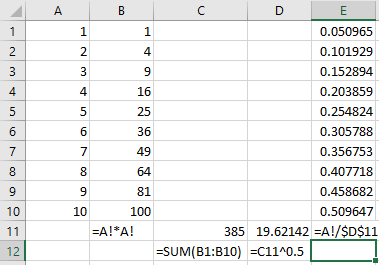
\includegraphics[width=7cm]{img/unitvector.png}
\end{center}

\medskip \noindent The Excel user must manually input the data, and additionally make space for the intermediate steps of the calculation. As the data becomes more diverse and the problem becomes more complicated, more work is required. Below is the equivalent function in Extend, written to work on any column vector that is passed in:

\begin{lstlisting}
	normalize_column_vector([m,1] arg) {
	  [m,1] squared_lengths := #arg * #arg, normalized := #arg / vector_norm;
	  vector_norm := sqrt(sum(squared_lengths));
	  return normalized;
	}
\end{lstlisting}

\medskip \noindent Another particularly interesting example is concatenating a row of strings of variable length with a common delimiter. This in an entirely manual operation for the spreadsheet user; a step-by-step attempt is shown below.

\begin{center}
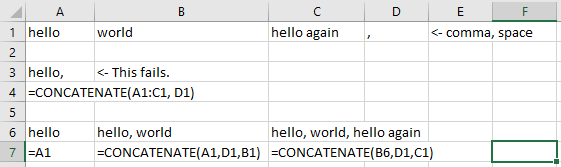
\includegraphics[width=9cm,height=3cm]{img/concatenation.png}
\end{center}

\medskip \noindent Performing a delimiter 'join' like the above can be performed in a simple program in Extend without knowing the size of the row.

\begin{lstlisting}
main(args){
	bar := {"Hello", "Goodbye", "Hello Again"};
	str := ", ";
	return foo(bar, str);\\ prints "Hello, Goodbye, Hello Again"
}

foo([1,n] colrange, str){
	[1,n] baz;
	baz[0,0] = #colrange;
	baz[0,1:] = baz[0,[-1]] + str + colrange[0,[0]];
	return print_endline(baz[0,-1]);
}
\end{lstlisting}

\medskip \noindent As evidenced above by simple examples, Extend offers flexibility that is significantly harder to achieve with conventional spreadsheet applications. As the nature of the data grows in complexity and variety, Extend's value increases.

\section{Writing Extend Code - The Basics}
Extend code can be written in a file that contains the conventional \texttt{.xtnd} extension. It consists of optional import statements and global variables, and an optional set of functions. Runnable Extend programs must contain a \texttt{main} function, and other functions can be written into the program as well.

\medskip \noindent
Below is a short tour of the features of Extend. More detail can be found in the next chapter - the Language Reference Manual.

	\subsection{Functions}
	Functions are commonplace in Extend. They are declared with the syntax \texttt{function\_name([optional\_dimensions] function\_arguments)\{...\}}. Below is the syntax of the \texttt{main} function, which is needed to run Extend code, within a simple Extend program.

	\begin{lstlisting}
	main(args){
			return 0;
	}
	\end{lstlisting}
	% Perhaps a more informative program - but not too difficult.

	\medskip \noindent
 	The return type of a function is a \textbf{range} of flexible size. \textbf{Ranges} will be discussed in a later section of this chapter. A function is composed of a series of statements, concluding with the return statement.
	Note that the \textbf{return} statement is always the last statement in the function.

		\subsubsection{Function Parameters}
		Function parameters consist of zero or more ranges, signed with an optional dimension. If the arguments have been written with dimensions, those dimensions will be verified at runtime.
		\begin{lstlisting}
			foo([m,n] arg){
				return m * n; \\ m and n initialized through arg1
			}

			bar([1,1] arg){
				return 0; \\ 1 by 1 ranges should be primitive data types. If arg is not, a runtime error will be thrown
			}
		\end{lstlisting}

	\subsection{Adjusting to Extend's Declarative Nature}
	The biggest difference between Extend and most traditional programming languages is that the concept of an imperative statement does not exist. An Extend function consists solely of variable declarations, formula assignments, and a return expression. When a function is called, its \texttt{return} expression is evaluated, along with the values of any variables that the return expression depends on. In a traditional imperative language, the order of operations is determined explicitly by the developer; in Extend, the order is determined implicitly by the desired result.

	\medskip \noindent The file below compiles and prints successfully.

	\begin{lstlisting}
		main(args){
			foo := "Hello World!";     // Combined variable declaration and formula assignment
			return print_endline(foo); // The return expression is a call to print_endline().
		}
	\end{lstlisting}

	\medskip \noindent However, this is not a legal Extend program:

	\begin{lstlisting}
		main(args){
			foo := "Hello World!"; // OK
			print_endline(foo);    // Not OK
			return foo;
		}
	\end{lstlisting}

	\medskip \noindent As illustrated, Extend only evaluates what is needed to produce the value required by \texttt{return}. Any non-essential declarations or formula assignments will be ignored by the program. If the user attempts to write statements like \texttt{print\_endline("Hello")} by itself, the program will not compile.

	\subsection{Data Types}
	Extend has three primitive data types: Numbers, Strings, and \texttt{empty}; and one composite type, Range. An example of each is shown below.

	\begin{lstlisting}
		myNumber := 5;
		myString := "Hello World";
		myEmpty  := empty;
		myRange  := {3, 4, "five";
							   "a", "b", "c"}
	\end{lstlisting}

	\subsection{Variables}
	In Extend, \texttt{variables} are composed of cells to which formulas are assigned. The first time (and only the first time!) an individual cell is referenced by an expression, its value is calculated according to its assigned formula. A cell's value is not calculated if the cell is never referred to, and is never recalculated; all cell values are immutable. A cell's value can be any of Extend's types, and different cells of a single variable can have different types.

	\begin{lstlisting}
		[1,2] foo; // Declares a variable with 1 row and 2 columns (2 cells total)
		[1,3] bar := 4; // Declares a variable with 1 row and 3 columns and
		                // assigns the literal value 4 as the formula for each cell
		[1,2] baz;                 // Declares a 1x2 variable baz
		baz[0,0] = "first cell";   // Assigns the literal "first cell" as the formula for the
		baz[0,1] = 1 + 1;          // first cell and the expression 1+1 for the second cell
		life := 6, universe := 7;  // Declares 1x1 variables life and universe
		answer := life * universe; // Declares a 1x1 variable the_answer and assigns
															 // the formula life * universe to its sole cell
		[1,10] half_and_half;			 // Declares a 1x10 variable half_and_half
		half_and_half[0,0:5] = "milk";		// Assigns "milk" to the first five cells
		half_and_half[0,5:10] = "cream";  // and "cream" to the second five cells
	\end{lstlisting}

	\medskip \noindent
	\textbf{Note} that we declare a variable and assign a formula to all of its cells in a single line with \texttt{:=}. If the variable has already been declared, a formula must be assigned using \texttt{=} instead of \texttt{:=}. As illustrated in this example, a single formula can be assigned to multiple cells of a variable with the slice syntax. The contents of the slice, as well as the dimensions of the variable, can be any expression that evaluates to a number, not just a literal number. For example, this code snippet assigns the dimensions based on the \texttt{how_big()} function and the formulas "left", "right", and "last" based on the \texttt{breakpoint()} function:

	\begin{lstlisting}
		breakpoint() {
			return 7;
		}
		how_big() {
			return 11;
		}
		foo_func() {
			[1,how_big()] foo;
			foo[0, :breakpoint()] = "left";
			foo[0, breakpoint():-1] = "right";
			foo[0, -1] = "last";
			return foo;
		}
	\end{lstlisting}

	\medskip \noindent
	This example also illustrates that the start (or end) index of a slice can be omitted if the developer wants the formula to apply from the beginning (or to the end) of the dimension, and that negative numbers can be used in a slice to count backwards from the end. As with all values in Extend, the dimensions of a variable, and the slices to which a formula applies, are immutable. The first time a variable is referred to (directly or indirectly) by the return expression, its dimensions and the formula assignment slices are computed; from that point on, they never change. In the example above, the how_big() function is invoked once, but the breakpoint() function is actually called twice: once for the "left" formula, and once for the "right" formula. 

		\subsubsection{The typeof operator}
		Extend offers a \texttt{typeof(expr)} operator, which takes and expression and returns Number, String, Range, or Empty.

	\subsection{Operators}
	Extend includes a comprehensive set of operators. Each category is listed in order of precedence. A more detailed explanation of each operator can be found in the Language Reference Manual.

		\subsubsection{Arithmetic Operators}
			\begin{itemize}
				\item Unary Operations: \texttt{-}
				\item Binary Operations: \texttt{**, *, /, \%, +, -}
			\end{itemize}

		\subsubsection{Bitwise Operators}
			\begin{itemize}
				\item Unary Operations: \texttt{\~}
				\item Binary Operations: \texttt{<<, >>, \&, |, \^}
			\end{itemize}

		\subsubsection{Boolean Operators}
			\begin{itemize}
				\item Unary Operations: \texttt{!}
				\item Binary Operations: \texttt{==, !=, <, >, <=, >=, \&\&, ||}
			\end{itemize}

		\subsubsection{String Concatenation}
		Note that the \texttt{+} symbol can be used to perform concatenation between two strings.

		\begin{lstlisting}
			"Hello " + "World\n"
		\end{lstlisting}

	\subsection{Conditionals}
	There are two types of conditionals: the if-then-else (ternary) conditional and a \texttt{switch} expression.

		\subsubsection{If-Then-Else}
		The two ways to write the ternary expression are as follows: \newline \newline
		C/Java style: \texttt{condition ? expr\_if\_true : expr\_if\_false} \newline \newline
		or: \newline \newline
		Spreadsheet style: \texttt{if(conditional, expr\_if\_true, expr\_if\_false)}

		\subsubsection{The Switch Expression}
		Below is an example of the switch expression used in a function:

		\begin{lstlisting}
			odd_or_even(foo){
				return switch(foo % 2) {
					case 0: "Even";
					case 1: "Odd";
					default: "Not an integer";
				};
			}
		\end{lstlisting}

	\medskip \noindent
	Ranges can also be declared as range literals. Rows are delineated by \texttt{;} and columns by \texttt{,}.

	\begin{lstlisting}
		foo := {"Hello", 1, 2; 3, 4, 5; 6, 7, 8} \\ Three rows, three columns.
	\end{lstlisting}

		\subsubsection{Range Slicing \& Selection}
		Python-style array-slicing syntax can be applied to ranges, which will return a subrange based on either absolute or relative indexing. All indices are zero-based.

		\begin{lstlisting}
			foo[0,2] \\ The cell in the first row, third column
			foo[0,:] \\ The range of cells in the first row
			foo[0,[1]] \\ The range in the column that is 1 column right of the left-hand-side cell.
			foo[,] \\ Cell in first row, first column if 1 by 1. If not, then relative first row and relative first column
		\end{lstlisting}

		\medskip \noindent
		More examples and detail can be found in the next chapter.

		\subsubsection{The Hash Operator}
		A common case for ranges in Excel is to perform calculations on specific cells. For example, \texttt{foo[,]} is commonly used to retrieve the cell that is being calculated on.
		Since this is a popular use case, the \texttt{\#} operator will perform the same functionality.

		\subsubsection{Application on Ranges}
		Extend, in the vein of spreadsheets, allows the programmer to apply functions cell-wise on a range. Using the \texttt{\#} operator, we can perform cell-wise multiplication across two ranges.

		\begin{lstlisting}
			foo([m,n] arg1, [m.n] arg2){
				[m,n] bar := #arg1 * #arg2; \\ Multiplies the cell in arg1 with the corresponding cell in arg2.
				return bar;
			}
		\end{lstlisting}

		\medskip \noindent
		This is an incredibly powerful aspect of Extend. Make sure to study it well!

		\subsubsection{Range Attribute Functions}
		Extend has the \texttt{row()} and \texttt{column()} functions, which respectively return the row and column of the cell that is being calculated at that point in time.
		There is also a \texttt{size(expr)} function, which returns a 1 by 2 range; the first cell contains the number of rows, and the second cell contains the number of columns.

	\subsection{Precedence Expressions}
	Precedence Expressions are used to force the evaluation of one expression before another. This is used when the order of operation is required for functions with side effects, such as the ones housed in Extend's standard library.
	The \texttt{->} operator is used to denote precedence.

	\begin{lstlisting}
		return print_func(4) -> 0; \\ print_func prints 4 to stdout before returning 0
	\end{lstlisting}

	\subsection{Import Statements}
	In Extend, you can import other Extend files at the top of your program via relative directory path. The use case is below:

	\begin{lstlisting}
		import "../programs/helloworld.xtnd"
	\end{lstlisting}

\section{Standard Library Functions}
Extend offers an assortment of standard library functions. Extend imports \texttt{stdlib.xtnd}, which has aggregated all the standard library functions for the user's disposal.

\medskip \noindent
While their usage will be covered in more length in the Language Reference Manual, here are some of the more useful standard library functions to remember.
	\subsection{Basic Functions}
		\subsubsection{The toString() Function}
		The \texttt{toString()} function takes a 1 by 1 range and renders its value as a string. This will return one of the primitive data types.

		\begin{lstlisting}
			return "Hello " + toString(14); \\ "Hello 14"
		\end{lstlisting}

		\subsubsection{Math Functions}
		Borrowing from C's standard library math functions, Extend offers: \texttt{sin, cos, tan, acos, asin, atan, sinh, cosh, tanh, exp, log, log10, sqrt, ceil, fabs} and \texttt{floor}.

		\begin{lstlisting}
			main(args){
				bar := sqrt(16);
				return write(STDOUT, toString(bar)) -> 0; \\ Prints 4 to stdout
			}
		\end{lstlisting}

	\subsection{File I/O}
	Extend has \texttt{open, close, read, and write} functions to interact with files. Usage is as follows:

	\begin{lstlisting}
		main(args){
		  return write(STDOUT, read(open("test_file.txt", "r"),5)) -> 0; \\ Writes 5 characters from test_file.txt to stdout
		}
	\end{lstlisting}

	\subsection{Plotting}
	Extend also offers the ability to export plots to a PNG file with the \texttt{plot} function.

	\begin{lstlisting}
		TODO: Demonstrate usage here.
	\end{lstlisting}

  %\chapter{Language Reference Manual}
  \input{Extend/tex/Intro}
  \input{Extend/tex/TypesAndLiterals}
  \input{Extend/tex/Expressions}
  \input{Extend/tex/Functions}
  \input{Extend/tex/StdLib}
  \input{Extend/tex/ExampleProgram}

  \chapter{Project Plan}

\section{Meetings}
Our goals were outlined by weekly meetings. We regularly met with Jacob Graff, our advisor throughout the development of Extend.
Jacob served as a sounding board whenever Extend's fundamental design philosophy was debated, and as a guide as we determined whether we were on track. We used any leftover time on those days to set goals for the upcoming week and pair program if time permitted.
\newline \newline
Our team also met weekly on Fridays to further discuss the progression of Extend. In the first half of the semester, the discussions were primarily philosophical, as decisions had to be made about the language grammar and behavior of certain Extend artifacts prior to development. In the second half, time was devoted to ironing out the development timeline, discussing bugs, and making compiler implementation decisions.

\section{Development Workflow}
  \begin{center}
  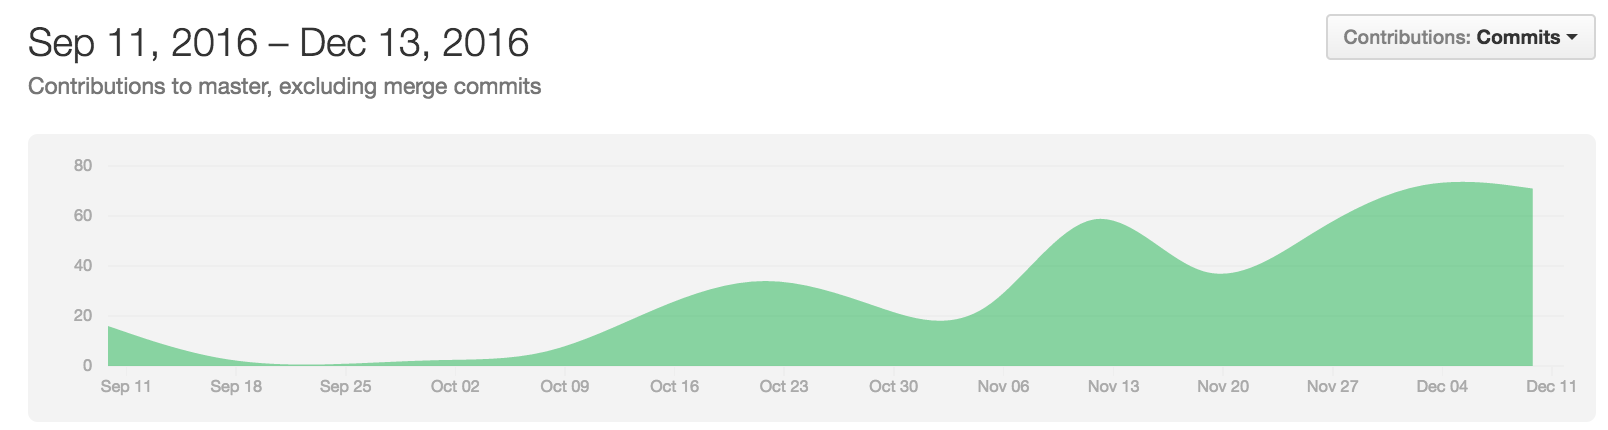
\includegraphics[width=.9\textwidth]{img/extend_git_graph.png}
  \end{center}

  \subsection{Github \& Travis CI}
  Our development and documentation were all done entirely through version control to maximize independent productivity.
  New features were introduced to the master branch through pull requests, and the team used this as a platform to peer review code to maximize code quality before such features entered production.

  \medskip \noindent
  An important aspect of development for us was continuous integration. Each pull request we made triggered a Travis build, which kept us informed regarding unexpected hiccups that sometimes arose during development. Travis CI ensured that new features were implemented with protecting the code base in mind, and provided quick visibility as to whether a new feature would break the existing build. Any changeset to the master branch must:

  \begin{enumerate}
    \item Pass Travis CI.
    \item Be approved by another member of the team.
    \item Be up to date with the master branch.
  \end{enumerate}

\section{Project Feature Completion Timeline}
Over the semester, we implemented our compiler from front end to back end, incorporating test cases throughout the way. Below are timestamps of our project progress throughout the semester.

  \begin{enumerate}
    \item Scanner (Early October)
    \item Parser (Mid October)
    \item Achieved Enlightenment \& Finalized Language Semantics (Late October)
    \item AST (Early November)
    \item Transformer and Semantic Analysis (Mid November)
    \item Code Generation (Late November)
    \item Standard Library and Regression Testing (Mid December)
    \item Gave Glorious Presentation to Professor Edwards (Mid December)
  \end{enumerate}


\subsection{Style Guide}
  None of the team members had any prior experience with Ocaml. Fundamentally we were developing a certain style in the process of creating the project. A few style choices were clear soon after starting to develop in Ocaml:
  \begin{itemize}
  \item Avoid deep nesting of functions
  \item Instead build better abstraction and reuse functions
  \item Use \textbf{let ... in} instead of \textbf{and}. While this creates a lot of closures, it helped us to develop quicker by not needing to restructure code for changes
  \item Use underscore for values you won't use any further. Llvm code generation inherently creates a lot of values where the return value is of no use. Therefore mark those return values with an underscore, since it hides the warning.
  \item Indent with spaces, not tabs. Indent by 2 for each level of nesting.
  \item Make intentions clear by naming return values, not by naming LLVM indermediate values.
  \end{itemize}
These few rules helped us to control our code very well.\newline
Further we were developing our runtime in C. We applied the following style rules:
  \begin{itemize}
  \item Indent with tabs.
  \item Stick to C99.
  \item Use \textbf{value\_p} for user facing functions.
  \item Make sure to exit gracefully.
  \end{itemize}

\section{Language Evolution}
Looking back at our original proposal, the language we delivered ended up surprisingly close. The biggest change was to allow strings and ranges as value types, which made the language immeasurably better. Initially, we wanted to only have Numbers; but allowing cells to contain ranges (composite values) and not just primitive values makes it a much more useful language. Otherwise, the syntax and semantics are very close to what was in our original proposal.

Our initial plan was to precalculate the dependencies among cells as best as possible at compile time and generate code accordingly. However, it quickly became clear that the language was better with runtime-determined cell dependencies and we therefore had to give up on a precomputed graph. We didn't have time in this class to implement an explicit stack as opposed to using recursion, but this could be overcome if it had to be.

Another fairly minor change was to eliminate the dimension signature for functions. As we played around with the language in the interpreter, it became clear that we weren't using them and it wasn't obvious why we would; they were dropped as a result.


  \subsection{The Interpreter}
  In our efforts to maximize our effectiveness when building the compiler, we additionally built a working interpreter to test the language semantics and run example Extend programs. This helped us determine language decisions at an earlier stage in the process, and helped us benchmark the success of our compiler by comparing the number of testcases passed by both.

\section{Team Member Responsibilities}

\begin{tabular}{ | l | l | l |}\hline
  Team Member  & Responsibilities      & GitHub Profile\\ \hline
  Jared Samet & design philosophy, semantic transformations, code generation  & \underline{\href{https://github.com/oracleofnj}{oracleofnj}}\\
  Nigel Schuster & development protocol, code generation, scripting  & \underline{\href{https://github.com/Neitsch}{Neitsch}}\\
  Ishaan Kolluri & initial LRM, Final Report, regression tests, stdlib functions, scripting & \underline{\href{https://github.com/ishaankolluri}{ishaankolluri}}\\
  Kevin Ye & initial scanner, regression tests, stdlib functions & \underline{\href{https://github.com/kevinye1}{kevinye1}}\\ \hline
\end{tabular}

	\medskip \noindent
\chapter{Git Logs}
Contributions\newline
Jared Samet 425 commits / 15,917 ++ / 12,151 --\newline
Nigel Schuster 320 commits / 6,258 ++ / 4,887 --\newline
Ishaan Kolluri 66 commits / 1,389 ++ / 726 --\newline
Kevin Ye 24 commits / 1,700 ++ / 633 --\newline
\begin{lstlisting}
23c2ae6 2016-12-17T13:00:05-05:00 GitHub: Merge pull request #123 from ExtendLang/size-asserts
4c51203 2016-12-17T11:59:30-05:00 oracleofnj: Right confusion
c05cf61 2016-12-17T11:52:34-05:00 oracleofnj: Fix import dir bug
39edbb4 2016-12-17T11:46:06-05:00 oracleofnj: Merge branch 'master' into size-asserts
339cb1f 2016-12-17T11:45:54-05:00 oracleofnj: Fix merge conflict
7462381 2016-12-17T11:44:50-05:00 GitHub: Merge pull request #122 from ExtendLang/split-stdlib
61ac8f2 2016-12-17T11:38:19-05:00 oracleofnj: Size asserts
606af9f 2016-12-17T11:22:36-05:00 oracleofnj: Transform asserts into more useful form; add calc of assert value to codegen
ee4f369 2016-12-17T10:40:17-05:00 oracleofnj: Combine asserts into a single expression
0f0f1c8 2016-12-17T10:38:56-05:00 Nigel Schuster: Added right and left to stdlib
fa43425 2016-12-17T10:30:23-05:00 oracleofnj: Split stdlib
824c53c 2016-12-17T10:11:13-05:00 Nigel Schuster: Added toUpper and toLower
ec24177 2016-12-17T10:02:30-05:00 Nigel Schuster: Implemented to and from ASCII
ab2e8f8 2016-12-17T09:15:39-05:00 GitHub: Merge pull request #116 from ExtendLang/line-plus
5d1610b 2016-12-17T09:08:57-05:00 GitHub: Merge branch 'master' into line-plus
df3a827 2016-12-17T09:08:48-05:00 GitHub: Merge pull request #117 from ExtendLang/cmd-args
32a3487 2016-12-17T09:02:27-05:00 GitHub: Merge branch 'master' into cmd-args
a8f9d33 2016-12-17T09:00:23-05:00 Nigel Schuster: Args
bfccf0c 2016-12-17T08:58:08-05:00 Nigel Schuster: Cut down line count for plus
a6bc89a 2016-12-17T08:48:31-05:00 GitHub: Merge pull request #114 from ExtendLang/only-new-string
5c96b7f 2016-12-17T08:03:27-05:00 GitHub: Merge pull request #109 from ExtendLang/unop-bitnot
3834210 2016-12-17T00:33:37-05:00 oracleofnj: Get rid of box string in favor of new_string_all_the_way, renamed new_string
375bea7 2016-12-16T23:56:35-05:00 oracleofnj: Merge branch 'unop-bitnot' into remove-interpreter
fb1bd77 2016-12-16T23:54:43-05:00 oracleofnj: Clean up; remove interpreter; change DimInt to DimOneByOne
539dd75 2016-12-16T23:46:35-05:00 GitHub: Merge branch 'master' into unop-bitnot
5668e53 2016-12-16T23:43:57-05:00 Nigel Schuster: Using lrint instead of fptosi
45691eb 2016-12-16T23:35:38-05:00 GitHub: Merge pull request #111 from ExtendLang/global-semant
2cdfb8b 2016-12-16T23:33:26-05:00 GitHub: Merge branch 'master' into global-semant
c9500d9 2016-12-16T23:33:14-05:00 GitHub: Merge pull request #112 from ExtendLang/remove-function-signatures
0c24f54 2016-12-16T23:25:23-05:00 oracleofnj: Remove return signature from grammar and all test cases
e7f2864 2016-12-16T23:03:53-05:00 oracleofnj: Merge branch 'cleanup-1' into global-semant
567507e 2016-12-16T22:53:20-05:00 oracleofnj: Check globals; use same symbol_table function for semant and codegen
55d8185 2016-12-16T22:00:30-05:00 Nigel Schuster: Removed comments and unneccessary files
629042f 2016-12-16T21:37:07-05:00 GitHub: Merge branch 'master' into unop-bitnot
48b139a 2016-12-16T21:34:09-05:00 Nigel Schuster: Implemented unary bitnot
39b02cd 2016-12-16T21:27:22-05:00 oracleofnj: Merge branch 'master' into global-semant
28c0983 2016-12-16T21:27:05-05:00 oracleofnj: Remove leftover printf
dc182df 2016-12-16T21:09:00-05:00 GitHub: Merge pull request #105 from ExtendLang/rg-eq
8cdf5c4 2016-12-16T19:31:26-05:00 oracleofnj: Expand test cases for range equality
41a3ccc 2016-12-16T19:18:44-05:00 GitHub: Merge branch 'master' into rg-eq
8dbebc1 2016-12-16T19:18:15-05:00 GitHub: Merge pull request #104 from ExtendLang/prevent-overlapping-formulas
c1431b5 2016-12-16T18:55:07-05:00 Nigel Schuster: Implemented basic subrange comparison
546536e 2016-12-16T18:47:12-05:00 oracleofnj: Detect overlapping formulas and give runtime error if present
3562e1b 2016-12-16T18:45:12-05:00 oracleofnj: Merge branch 'sr-val-fix' into prevent-overlapping-formulas
8713fa0 2016-12-16T18:42:40-05:00 oracleofnj: Checking
77d80b9 2016-12-16T18:26:31-05:00 Nigel Schuster: Fixed check for subrange
962c744 2016-12-16T12:09:00-05:00 GitHub: Merge pull request #101 from ExtendLang/finishing-these-range-literals
f234e00 2016-12-16T00:21:06-05:00 oracleofnj: Merge branch 'more-stdlib-functions' into finishing-these-range-literals
c9246ce 2016-12-16T00:20:59-05:00 oracleofnj: testing testing
6914039 2016-12-16T00:14:09-05:00 oracleofnj: Third time's the charm
4617e44 2016-12-16T00:01:12-05:00 oracleofnj: It compiles now
1d8e290 2016-12-15T23:42:43-05:00 oracleofnj: Fingers crossed
c9d28d3 2016-12-15T21:50:01-05:00 oracleofnj: Move all initializations into their own function; only box strings once
1cfdd16 2016-12-15T18:47:30-05:00 oracleofnj: Merge branch 'master' into more-stdlib-functions
19c2beb 2016-12-15T18:40:12-05:00 oracleofnj: Try a couple more things out
845cb04 2016-12-15T18:33:07-05:00 GitHub: Merge pull request #96 from ExtendLang/ternary-fix
4bfb3bc 2016-12-15T18:23:00-05:00 oracleofnj: Merge branch 'ternary-fix' into more-stdlib-functions
ae55ca4 2016-12-15T18:21:58-05:00 oracleofnj: Define cell_row, cell_col
30a5db6 2016-12-15T18:19:56-05:00 oracleofnj: Merge branch 'ternary-fix' into more-stdlib-functions
b9f1f10 2016-12-15T18:17:53-05:00 oracleofnj: What is truth?
ac84c2f 2016-12-15T18:15:37-05:00 oracleofnj: Fix ternary to work properly with ranges
1f57d91 2016-12-15T17:03:26-05:00 oracleofnj: Look at this one
437ba46 2016-12-15T16:56:04-05:00 oracleofnj: Try this one
f0edf5b 2016-12-15T16:46:52-05:00 oracleofnj: Fixing bug
5ba31e6 2016-12-15T14:17:52-05:00 GitHub: Merge pull request #94 from ExtendLang/nan-inf
67c5739 2016-12-15T14:17:46-05:00 GitHub: Merge pull request #93 from ExtendLang/type-typeof
48a3d5c 2016-12-15T14:05:37-05:00 oracleofnj: Improve test case
8f08227 2016-12-15T13:58:46-05:00 oracleofnj: Add isNaN and isInfinite to stdlib
cbeec74 2016-12-15T13:30:31-05:00 oracleofnj: Rename token
9582228 2016-12-15T13:18:09-05:00 oracleofnj: Rename type to typeof
d1422c7 2016-12-15T10:42:19-05:00 GitHub: Merge pull request #92 from ExtendLang/compiler
66689bb 2016-12-15T09:08:56-05:00 Nigel Schuster: added working directory option, doing testing completely in tmp
a13ae93 2016-12-15T09:08:31-05:00 GitHub: Merge pull request #91 from ExtendLang/sizeof
a31add9 2016-12-15T09:08:13-05:00 GitHub: Merge pull request #90 from ExtendLang/subselect-C-side
2e67e06 2016-12-15T09:01:06-05:00 Nigel Schuster: Added option to specify compiler, using clang
c171450 2016-12-15T02:33:48-05:00 oracleofnj: SizeOf
c168044 2016-12-15T00:48:35-05:00 oracleofnj: Add row(), column() to codegen, add print_endline() to stdlib.xtnd
bf9426d 2016-12-15T00:27:13-05:00 oracleofnj: Print subrange
407ce41 2016-12-14T23:02:02-05:00 oracleofnj: Merge in subrange_string
756ea8e 2016-12-14T22:51:00-05:00 oracleofnj: Ranges
27a8e79 2016-12-14T22:16:13-05:00 oracleofnj: Resolve RHS slice
876d056 2016-12-14T22:02:56-05:00 oracleofnj: Resolve RHS index
b59e022 2016-12-14T21:46:00-05:00 Nigel Schuster: Added method to print subragne as string
a7d53a8 2016-12-14T19:55:38-05:00 oracleofnj: Merge branch 'master' into subselect-C-side
362e85b 2016-12-14T19:55:23-05:00 GitHub: Merge pull request #88 from ExtendLang/subselect
4912fa3 2016-12-14T19:40:10-05:00 oracleofnj: Add debug print info for slice structures
c1b33f4 2016-12-14T18:58:45-05:00 oracleofnj: Builder to end all builders
5d400c2 2016-12-14T18:55:06-05:00 oracleofnj: Add selection builders
29f6e28 2016-12-14T18:20:51-05:00 oracleofnj: Make additional infix operator for populating structure element
046d096 2016-12-14T17:49:19-05:00 oracleofnj: Set up RHS slice types
b25c2f5 2016-12-14T16:49:17-05:00 GitHub: Merge pull request #87 from ExtendLang/make-a-selection
7a12082 2016-12-14T16:43:38-05:00 oracleofnj: Move selection test cases back into inputs
e2c08d5 2016-12-14T16:31:00-05:00 oracleofnj: Make IDs work with deref_subrange
02f2f0c 2016-12-14T15:21:31-05:00 GitHub: Merge pull request #86 from ExtendLang/include-stdlib
8b0503f 2016-12-14T15:18:14-05:00 GitHub: Merge branch 'master' into include-stdlib
1f034a0 2016-12-14T15:17:52-05:00 GitHub: Merge pull request #84 from ExtendLang/math-linker
1e6dd91 2016-12-14T14:58:44-05:00 oracleofnj: Add expected output for slurp
ff1a5e3 2016-12-14T14:53:38-05:00 oracleofnj: Remove extend_ prefix from all sample code
81a2828 2016-12-14T14:48:38-05:00 oracleofnj: Automatically add extend_ prefix to external functions
dcc1ed3 2016-12-14T14:30:52-05:00 oracleofnj: Fix samples
9b2c28f 2016-12-14T12:39:45-05:00 oracleofnj: Include stdlib automatically
13650ce 2016-12-14T12:35:21-05:00 Nigel Schuster: Merge branch 'math-linker' of https://github.com/ExtendLang/Extend into math-linker
2e0d90d 2016-12-14T12:35:06-05:00 Nigel Schuster: Merge branch 'math-linker' of https://github.com/ExtendLang/Extend into math-linker
83c689e 2016-12-14T12:34:14-05:00 Nigel Schuster: Merge branch 'math-linker' of https://github.com/ExtendLang/Extend into math-linker
127f600 2016-12-14T12:34:07-05:00 Nigel Schuster: Include sys/resources
b34d97a 2016-12-14T12:03:44-05:00 GitHub: Merge branch 'master' into math-linker
8297f33 2016-12-14T12:01:47-05:00 GitHub: Merge pull request #85 from ExtendLang/put-lt-back
6b0c74f 2016-12-14T11:33:45-05:00 Nigel Schuster: Include sys/resources
37470e9 2016-12-14T11:14:06-05:00 oracleofnj: Put back LT, comment out sys/time.h
6bde590 2016-12-14T11:12:16-05:00 Nigel Schuster: Increasing stack size
6acc621 2016-12-14T11:03:31-05:00 Nigel Schuster: Disabled linking math when creating an intermediate
d87b73c 2016-12-14T10:51:58-05:00 GitHub: Merge pull request #82 from ExtendLang/hard-to-repro-bug
d126e3c 2016-12-14T00:51:00-05:00 oracleofnj: Try with time.h instead of sys/time.h
a535612 2016-12-14T00:48:35-05:00 oracleofnj: Remove lrints
e844853 2016-12-14T00:34:37-05:00 oracleofnj: Initialize all variables and remove pointer math; bug appears fixed
4c1a421 2016-12-13T22:55:07-05:00 oracleofnj: Some formula is weird
5dbd409 2016-12-13T22:43:19-05:00 oracleofnj: Merge branch 'hard-to-repro-bug' of https://github.com/ExtendLang/Extend into hard-to-repro-bug
879eaf3 2016-12-13T22:43:17-05:00 oracleofnj: Testing
37f5ce2 2016-12-13T22:42:40-05:00 GitHub: Merge pull request #83 from ExtendLang/rounding-for-read
a1cfc5a 2016-12-13T22:34:21-05:00 Nigel Schuster: Added rounding at several places
e20f7e4 2016-12-13T21:36:13-05:00 oracleofnj: Half the time it works
61bc9b6 2016-12-13T20:33:27-05:00 GitHub: Merge pull request #81 from ExtendLang/fix-em-all
4a810df 2016-12-13T19:34:29-05:00 Nigel Schuster: Corrected testcase outputs
ae5b8a8 2016-12-13T19:08:43-05:00 GitHub: Merge pull request #80 from ExtendLang/select
70b2704 2016-12-13T19:02:32-05:00 oracleofnj: No C99
15fd762 2016-12-13T18:42:21-05:00 oracleofnj: Merge branch 'master' into select
8e6e9ba 2016-12-13T18:42:05-05:00 GitHub: Merge pull request #78 from ExtendLang/unop-unary-minus
7a93885 2016-12-13T18:41:49-05:00 oracleofnj: Calculate all formula indices
07e63dc 2016-12-13T18:19:58-05:00 oracleofnj: Properly build instantiate var
1a29129 2016-12-13T17:24:16-05:00 oracleofnj: Replace bools with chars for compatibility between C and LLVM
12e78a3 2016-12-13T17:17:54-05:00 oracleofnj: Added debug output
a483282 2016-12-13T16:13:30-05:00 oracleofnj: Merge branch 'master' into unop-unary-minus
f8c9b43 2016-12-13T16:13:09-05:00 oracleofnj: Make TypeOf work
8146d04 2016-12-13T16:12:17-05:00 GitHub: Merge pull request #75 from ExtendLang/fix-more-tc
94afc93 2016-12-13T16:02:35-05:00 Nigel Schuster: Corrected expected TC
f6f8276 2016-12-13T16:00:59-05:00 Nigel Schuster: Fixed string.xtnd file
dcd5766 2016-12-13T15:44:38-05:00 GitHub: Merge pull request #74 from ExtendLang/fix-tc
bfe1c07 2016-12-13T15:39:45-05:00 oracleofnj: Merge branch 'master' into unop-unary-minus
d9abfc0 2016-12-13T15:38:38-05:00 GitHub: Merge branch 'master' into fix-tc
50ed49c 2016-12-13T15:38:04-05:00 oracleofnj: Merging in main
23328f1 2016-12-13T15:37:18-05:00 GitHub: Merge pull request #73 from ExtendLang/and-or-xor
324779a 2016-12-13T15:32:26-05:00 Nigel Schuster: Corrected expected value
fafe2e6 2016-12-13T15:29:21-05:00 Nigel Schuster: Fixed string tc
022f05c 2016-12-13T15:23:59-05:00 Nigel Schuster: Fixed testcase
b12fe37 2016-12-13T15:18:57-05:00 Nigel Schuster: Implemented and, or and xor
90cbaa0 2016-12-13T15:16:31-05:00 Nigel Schuster: Added left and right shift
571ee7e 2016-12-13T14:56:05-05:00 Nigel Schuster: Merge branch 'power' of https://github.com/ExtendLang/Extend into power
aeab40d 2016-12-13T14:55:57-05:00 Nigel Schuster: Removed unneccessary level of indirection
e377567 2016-12-13T14:53:28-05:00 GitHub: Merge branch 'master' into power
6ad8512 2016-12-13T14:53:11-05:00 GitHub: Merge pull request #69 from ExtendLang/unop-unary-minus
71f395d 2016-12-13T14:46:27-05:00 Nigel Schuster: Power to the people of Extend
6a04209 2016-12-13T14:45:46-05:00 oracleofnj: Fix merge conflict
edb0ecc 2016-12-13T14:43:32-05:00 oracleofnj: Add unary minus
668a0eb 2016-12-13T14:37:19-05:00 GitHub: Merge pull request #68 from ExtendLang/mod-div
866b68f 2016-12-13T14:32:18-05:00 Nigel Schuster: Added modulo and division operation
46d5aa6 2016-12-13T14:26:35-05:00 oracleofnj: Merge branch 'master' into unop-typeof
84dfc33 2016-12-13T14:26:25-05:00 Nigel Schuster: Crunched some code
76210eb 2016-12-13T14:26:18-05:00 oracleofnj: Start on it
f4d5a81 2016-12-13T14:22:12-05:00 Nigel Schuster: Merge branch 'master' into simplification
f873242 2016-12-13T14:21:26-05:00 GitHub: Merge pull request #65 from ExtendLang/subtraction
fc94112 2016-12-13T14:20:35-05:00 Nigel Schuster: Added multiplication
6c26c2c 2016-12-13T14:19:07-05:00 GitHub: Merge branch 'master' into subtraction
4afd78e 2016-12-13T14:18:55-05:00 GitHub: Merge pull request #64 from ExtendLang/refactor-boolean-binops
d4d4388 2016-12-13T14:15:58-05:00 GitHub: Merge branch 'master' into refactor-boolean-binops
bd90241 2016-12-13T14:14:17-05:00 GitHub: Merge branch 'master' into subtraction
4042259 2016-12-13T14:13:09-05:00 Nigel Schuster: Added subtraction
663f399 2016-12-13T14:12:57-05:00 oracleofnj: Remove wildcard from BinOp pattern match
82a3db2 2016-12-13T14:11:31-05:00 Nigel Schuster: Merge branch 'master' into subtraction
1bf6bed 2016-12-13T14:09:47-05:00 oracleofnj: Add TransformedAway exception for LogAnd and LogOr
c7d4162 2016-12-13T14:02:13-05:00 GitHub: Merge pull request #63 from ExtendLang/more-binops
952778e 2016-12-13T14:01:54-05:00 oracleofnj: Change Lt, Lte in grammar; implement GTE
97821c8 2016-12-13T13:47:52-05:00 oracleofnj: GT
1e1f973 2016-12-13T13:44:36-05:00 Nigel Schuster: Subtraction
e0a883a 2016-12-13T13:37:57-05:00 oracleofnj: Remove NotEq from AST since != is parsed to UnOp(LogNot,BinOp(Eq,...))
cc40008 2016-12-13T12:49:33-05:00 GitHub: Merge pull request #60 from ExtendLang/addition2
7123ebc 2016-12-13T12:41:09-05:00 GitHub: Merge branch 'master' into addition2
a656f57 2016-12-13T12:38:12-05:00 GitHub: Merge pull request #61 from ExtendLang/debug-unop
eb134b3 2016-12-13T12:29:53-05:00 Nigel Schuster: Moved testcases
044c6bd 2016-12-13T12:29:07-05:00 Nigel Schuster: Fixed off by one error
a64cc15 2016-12-13T12:14:45-05:00 oracleofnj: Add Debug expr
59858a0 2016-12-13T11:33:12-05:00 oracleofnj: Whoops no space
0426f34 2016-12-13T11:30:26-05:00 oracleofnj: Add test case
49ffa86 2016-12-13T11:19:14-05:00 GitHub: Merge branch 'master' into addition2
81533f4 2016-12-13T11:13:44-05:00 GitHub: Merge pull request #59 from ExtendLang/equal-rights
3cdaa5a 2016-12-13T11:12:41-05:00 Nigel Schuster: String addition
64d1760 2016-12-13T11:04:55-05:00 oracleofnj: Wake up please, GitHub
840aeaf 2016-12-13T10:48:03-05:00 oracleofnj: Remove usage demonstration
61ff439 2016-12-13T03:26:35-05:00 oracleofnj: Add string equality and test cases
f3112e9 2016-12-13T01:57:10-05:00 oracleofnj: Reduce cut & paste
08ce677 2016-12-13T01:35:46-05:00 oracleofnj: Remove obsolete testing file
ae8a07e 2016-12-13T01:23:26-05:00 oracleofnj: Merge branch 'print_value_p' into equal-rights
6090713 2016-12-13T01:22:47-05:00 oracleofnj: Use correct printf specifier
862b38c 2016-12-13T01:19:14-05:00 oracleofnj: Merge branch 'print_value_p' into equal-rights
5e913ad 2016-12-13T01:16:07-05:00 oracleofnj: Add debug_print; remove print statement that was causing us to falsely pass test cases from to_string; show usage in UnOp(Neg)
50281b1 2016-12-13T00:47:28-05:00 oracleofnj: Numeric equality
0f76aa4 2016-12-12T22:30:15-05:00 oracleofnj: Remove print flags
200b8b6 2016-12-12T22:16:15-05:00 GitHub: Merge pull request #57 from ExtendLang/addition2
da7c543 2016-12-12T12:43:31-05:00 Nigel Schuster: Setting flag for addition
7e7276b 2016-12-12T12:37:35-05:00 Nigel Schuster: Merge branch 'master' into addition2
8834635 2016-12-12T10:18:51-05:00 GitHub: Merge pull request #55 from ExtendLang/runtime
53ae9e0 2016-12-12T10:06:24-05:00 GitHub: Merge branch 'master' into runtime
6ed303e 2016-12-12T09:43:57-05:00 GitHub: Merge pull request #56 from ExtendLang/truthy-fix
ae49ce6 2016-12-12T01:15:29-05:00 oracleofnj: Remove extra file
7fe6a22 2016-12-12T01:11:53-05:00 oracleofnj: Falsey fix
d1e196d 2016-12-12T00:23:13-05:00 Nigel Schuster: Extracted runtime into seperate file
ecc620e 2016-12-12T00:17:06-05:00 GitHub: Merge pull request #54 from ExtendLang/final-draft-for-real
4c8caa5 2016-12-12T00:09:16-05:00 GitHub: Merge branch 'master' into final-draft-for-real
04d3b57 2016-12-12T00:00:29-05:00 GitHub: Merge pull request #39 from ExtendLang/more-lrm-ed
39025b0 2016-12-11T23:59:18-05:00 Nigel Schuster: Fixed examples, made small corrections
a875b41 2016-12-11T23:51:30-05:00 GitHub: Merge pull request #53 from ExtendLang/truthy
616dd34 2016-12-11T23:15:54-05:00 oracleofnj: Merge branch 'master' into truthy
0fa8255 2016-12-11T23:14:42-05:00 oracleofnj: Apparently still needs some work
78584d7 2016-12-11T23:09:07-05:00 oracleofnj: Thanks a lot Travis
b5673d2 2016-12-11T22:51:52-05:00 oracleofnj: TERRRRRRRRR NARRRRRRR EEEEEEEEEEEEEEEEEEE
b81bc1b 2016-12-11T22:04:25-05:00 oracleofnj: Maybe Truthy
b95d14f 2016-12-11T21:02:28-05:00 GitHub: Merge pull request #50 from ExtendLang/builder-hotfix
6dea96f 2016-12-11T20:40:47-05:00 oracleofnj: So many builders
8aa125f 2016-12-11T20:15:52-05:00 Nigel Schuster: Made som rpgroess
2a905c7 2016-12-11T19:15:47-05:00 GitHub: Merge pull request #47 from ExtendLang/function-parameter
2bc6c85 2016-12-11T19:11:33-05:00 oracleofnj: Add combined test case
860a11b 2016-12-11T19:04:35-05:00 oracleofnj: Merge branch 'master' into function-parameter
8c3499e 2016-12-11T19:03:39-05:00 oracleofnj: Remove extraneous printlines
99418c0 2016-12-11T19:02:31-05:00 oracleofnj: Make function parameters work
6c00a72 2016-12-11T18:45:46-05:00 Nigel Schuster: Some progress
387559b 2016-12-11T18:39:00-05:00 oracleofnj: First attempt
18fc1be 2016-12-11T18:08:11-05:00 GitHub: Merge pull request #45 from ExtendLang/empty
f7e9be8 2016-12-11T16:30:05-05:00 GitHub: Merge branch 'master' into empty
f1dd8a5 2016-12-11T16:18:44-05:00 GitHub: Merge pull request #46 from ExtendLang/actually-make-global-scope
50366f4 2016-12-11T15:38:05-05:00 oracleofnj: Make sure locals are properly masking globals
046c7cc 2016-12-11T15:30:53-05:00 oracleofnj: Make globals work, fix bug
a844a46 2016-12-11T15:14:09-05:00 oracleofnj: So close
18db166 2016-12-11T15:05:42-05:00 GitHub: Merge branch 'master' into empty
67849f0 2016-12-11T15:01:52-05:00 oracleofnj: Make the global scope object
393d02c 2016-12-11T14:25:02-05:00 Nigel Schuster: Implemented empty, small flag setting fix
3c4681d 2016-12-11T13:31:12-05:00 GitHub: Merge pull request #44 from ExtendLang/float-display-hotfix
7be1001 2016-12-11T13:26:55-05:00 GitHub: Merge branch 'master' into float-display-hotfix
abcffd0 2016-12-11T13:19:05-05:00 GitHub: Merge pull request #42 from ExtendLang/encapsulate-build-scope
556da44 2016-12-11T13:18:15-05:00 oracleofnj: Floating point math hotfix
0ad195e 2016-12-11T12:42:42-05:00 oracleofnj: Merge branch 'master' into encapsulate-build-scope
9caf464 2016-12-11T12:41:40-05:00 oracleofnj: Encapsulate a little more of building the scope
d65aad4 2016-12-11T12:09:28-05:00 GitHub: Merge pull request #40 from ExtendLang/make-global-scope
0f5a6ba 2016-12-11T12:04:05-05:00 oracleofnj: Merge branch 'master' into make-global-scope
56b58d9 2016-12-11T12:01:28-05:00 oracleofnj: Encapsulate build_var_defns
f25e5b3 2016-12-11T11:43:19-05:00 oracleofnj: Only construct var_defns once
9cee2fc 2016-12-11T10:07:36-05:00 Nigel Schuster: Testcases (#38)
f3f4bef 2016-12-11T00:45:44-05:00 oracleofnj: Make global variable to hold vardefns
a0ed757 2016-12-10T23:31:38-05:00 Nigel Schuster: Edited explanation for row() and column()
7c50ef2 2016-12-10T23:27:07-05:00 Nigel Schuster: Added info for strings
738e41b 2016-12-10T23:24:20-05:00 Nigel Schuster: Added boolean example
5377fdf 2016-12-10T23:19:26-05:00 Nigel Schuster: Added arithmetic example
a8f4ad9 2016-12-10T21:28:18-05:00 oracleofnj: Isolate the part of building a scope for reuse with global variables
58f7a4d 2016-12-10T18:05:01-05:00 Nigel Schuster: Performing copy before returning, so that memory can be freed with alloca
c0e56aa 2016-12-10T17:07:00-05:00 GitHub: Merge pull request #37 from ExtendLang/dereference
a4b35df 2016-12-10T16:42:17-05:00 Nigel Schuster: Removed obsolete methods
cf08a8c 2016-12-10T16:36:20-05:00 GitHub: Merge branch 'master' into dereference
ef0e5e7 2016-12-10T16:36:03-05:00 GitHub: Merge pull request #36 from ExtendLang/comp-warn
0177dc2 2016-12-10T16:35:50-05:00 GitHub: Merge pull request #35 from ExtendLang/linker
127f99d 2016-12-10T16:35:41-05:00 GitHub: Merge pull request #34 from ExtendLang/rel-import
b2e881d 2016-12-10T16:35:31-05:00 GitHub: Merge pull request #33 from ExtendLang/ts-fix
ce833d4 2016-12-10T16:14:34-05:00 Nigel Schuster: Dereferencing 1x1 subrange
e259556 2016-12-10T13:53:12-05:00 Nigel Schuster: Removed nodefaultlibs directive
09c3961 2016-12-10T13:50:19-05:00 Nigel Schuster: Modified linker to work for travis
36d662a 2016-12-10T13:37:27-05:00 Nigel Schuster: Attempt to link math
2d4564a 2016-12-10T13:22:14-05:00 Nigel Schuster: Linking math library
38ba6e6 2016-12-10T13:18:39-05:00 Nigel Schuster: Suppressing compiler warnings
9deac9b 2016-12-10T13:06:39-05:00 Nigel Schuster: Modified compile script. Removed debug output
d35607b 2016-12-10T13:04:30-05:00 Nigel Schuster: Simpler testscript
d37dac2 2016-12-10T12:36:45-05:00 Nigel Schuster: Fixed duplicate import issue
31c26bc 2016-12-10T12:30:29-05:00 Nigel Schuster: Added cmd args to link file
a350720 2016-12-10T11:40:50-05:00 Nigel Schuster: Switched import style from root directory to relative path
90e39b0 2016-12-10T11:24:19-05:00 Nigel Schuster: Fixed issue in testscript that might report false results when it fails early
718ecd3 2016-12-10T03:09:18-05:00 oracleofnj: Some changes to LRM; add if(a,b,c)
6a8f836 2016-12-09T18:29:22-05:00 GitHub: Merge pull request #24 from ExtendLang/final-draft-lrm
fc886a9 2016-12-09T18:23:52-05:00 oracleofnj: Merge branch 'final-draft-lrm'
cda63cb 2016-12-09T18:23:24-05:00 oracleofnj: Fix merge conflict
eac9e77 2016-12-09T18:04:08-05:00 GitHub: Merge pull request #29 from ExtendLang/refactor
fe825f4 2016-12-09T17:55:39-05:00 oracleofnj: Compact last bit
b02dbbe 2016-12-09T17:49:00-05:00 oracleofnj: Give formula functions names
edd7aa4 2016-12-09T17:40:57-05:00 Nigel Schuster: Removed artifcats
9b49e20 2016-12-09T17:37:59-05:00 Nigel Schuster: Fixed I/O testcases
a4ad4b1 2016-12-09T17:18:13-05:00 Nigel Schuster: Merge
b07398b 2016-12-09T17:17:19-05:00 Nigel Schuster: Added macro for function definition
ed01567 2016-12-09T17:17:06-05:00 oracleofnj: Make sizeof not break tests
a0a7054 2016-12-09T17:01:20-05:00 oracleofnj: Use symbol table
56fd61b 2016-12-09T16:11:10-05:00 oracleofnj: Merge branch 'refactor' of https://github.com/ExtendLang/Extend into refactor
38aedba 2016-12-09T16:10:35-05:00 oracleofnj: Create symbol table
dfb702e 2016-12-09T16:01:08-05:00 Nigel Schuster: Converted more to value_p from subrange_p
e963186 2016-12-09T15:42:35-05:00 Nigel Schuster: Made example TC work
eb76234 2016-12-09T11:14:58-05:00 Nigel Schuster: Made Hello World work again
08aeb70 2016-12-09T02:13:09-05:00 oracleofnj: Done for the night
cb39114 2016-12-09T01:35:36-05:00 oracleofnj: More refactoring
7974bbd 2016-12-08T23:53:31-05:00 oracleofnj: Banish the term extern
49af972 2016-12-08T23:45:30-05:00 oracleofnj: Add a couple comments
0fbf461 2016-12-08T21:52:24-05:00 oracleofnj: Get my bearings
5ecb599 2016-12-08T19:47:51-05:00 Nigel Schuster: Added some documentation
65066fc 2016-12-08T12:18:57-05:00 Nigel Schuster: Added name display for variable
fb18949 2016-12-07T23:44:17-05:00 oracleofnj: Merge branch 'master' into final-draft-lrm
4aab3dc 2016-12-07T23:43:25-05:00 oracleofnj: Update PDF
ed44d27 2016-12-07T23:43:01-05:00 oracleofnj: Fix failing test cases
9354fa7 2016-12-07T23:06:36-05:00 oracleofnj: Final draft candidate
78649f4 2016-12-07T18:09:46-05:00 oracleofnj: Almost done
05ded19 2016-12-07T15:47:52-05:00 oracleofnj: More work
f985cc8 2016-12-07T12:14:59-05:00 Nigel Schuster: Merge branch 'finish-transformations' into get-val-rev
4b58ce9 2016-12-07T12:13:23-05:00 Nigel Schuster: Tried to add more instructions
0722412 2016-12-07T11:32:11-05:00 oracleofnj: Working
099efe7 2016-12-07T10:48:35-05:00 Nigel Schuster: Making progress on evaluating dimensions
fa09df7 2016-12-07T09:51:23-05:00 Nigel Schuster: Finally it works
cbb0577 2016-12-07T02:35:06-05:00 oracleofnj: Still WIP
e3c9436 2016-12-07T00:44:22-05:00 oracleofnj: WIP
b265e74 2016-12-07T00:41:23-05:00 Nigel Schuster: test commit to look at
18bb182 2016-12-07T00:35:06-05:00 oracleofnj: Still work in progress
a4554c0 2016-12-06T23:14:32-05:00 Nigel Schuster: At least it compiles
3432484 2016-12-06T22:42:22-05:00 Nigel Schuster: Getting closer. Need to add var_defn wrapper in build_formula
05145ca 2016-12-06T21:10:11-05:00 Nigel Schuster: Minor fix
af69b92 2016-12-06T17:23:45-05:00 oracleofnj: More updates
a65c24e 2016-12-06T16:14:10-05:00 oracleofnj: Merge branch 'master' into finish-transformations
85a4ccb 2016-12-06T16:12:31-05:00 oracleofnj: LRM update part 1
174a7b8 2016-12-06T11:09:31-05:00 Nigel Schuster: Made partial progress on implementing variable instanciation and such
90fc58e 2016-12-05T22:14:41-05:00 GitHub: Merge pull request #23 from ExtendLang/read-empty
767851d 2016-12-05T16:18:17-05:00 Nigel Schuster: Finished C side implementation of getVal
6b837d4 2016-12-05T16:06:34-05:00 Nigel Schuster: Merge branch 'master' into get-val
04c2c65 2016-12-05T15:53:35-05:00 oracleofnj: Add slurp by passing 0 max bytes
d8cf316 2016-12-05T14:46:46-05:00 oracleofnj: Start handling empty
910bd01 2016-12-05T14:27:07-05:00 GitHub: Merge pull request #21 from ExtendLang/fileio
1ce7f83 2016-12-05T14:18:41-05:00 oracleofnj: Create patch file
88480fb 2016-12-05T13:36:28-05:00 GitHub: Merge branch 'master' into fileio
29d02d9 2016-12-05T13:34:27-05:00 oracleofnj: Fix merge conflict - keep expr_loc
52e7a8a 2016-12-05T13:32:54-05:00 GitHub: Merge pull request #22 from ExtendLang/rm-micro
bfa906b 2016-12-05T13:28:03-05:00 oracleofnj: Fix off-by-one bug
eb8dd71 2016-12-05T13:20:03-05:00 oracleofnj: Address issues
f1b11ee 2016-12-05T12:46:35-05:00 Nigel Schuster: Skeleton for get_val
e4e5e26 2016-12-05T09:25:17-05:00 Nigel Schuster: Removed microc reference implementation
270da2b 2016-12-05T02:40:59-05:00 GitHub: Merge branch 'master' into fileio
b928e98 2016-12-05T02:40:10-05:00 Ishaan: Remove bloat
894b511 2016-12-05T02:32:49-05:00 Ishaan: Added testcase
62b8e83 2016-12-05T02:30:16-05:00 Ishaan: Added fwrite implementation
77a23ae 2016-12-05T01:39:30-05:00 Ishaan: Added read
46e9b58 2016-12-05T00:07:16-05:00 Ishaan: Make refactoring changes and new helpers
a5b9066 2016-12-04T14:00:30-05:00 GitHub: Merge pull request #20 from ExtendLang/lhs-all-ids
35e9471 2016-12-04T13:38:44-05:00 oracleofnj: Put back Id(s) as it was
641d454 2016-12-04T13:36:36-05:00 oracleofnj: Always transform to ID on LHS, even for LitInts
0e8398f 2016-12-04T13:23:27-05:00 oracleofnj: Transform all LHS expressions including integers to IDs; check for strings or range literals and disallow
f47f2ba 2016-12-04T10:30:44-05:00 oracleofnj: Add error handling to close() and add a couple test cases
e95a95a 2016-12-04T10:07:01-05:00 oracleofnj: Add assertSingleNumber and get_number to eliminate more copy & paste
543e720 2016-12-04T09:47:03-05:00 oracleofnj: Add new_number() to eliminate some copy and paste
d7f10c9 2016-12-04T02:31:03-05:00 Ishaan: Tentative drafts of fileio functions
7d81e43 2016-12-04T00:15:20-05:00 oracleofnj: add diagnostic prinfs
868d9a4 2016-12-03T23:46:01-05:00 Ishaan: Cleanup
aa1e014 2016-12-03T23:42:46-05:00 Ishaan: Add file pointer array
88d05de 2016-12-03T18:38:34-05:00 Ishaan: Working on fopen
36f5848 2016-12-03T14:07:39-05:00 oracleofnj: Merge branch 'master' into finish-transformations
2ae2b83 2016-12-03T14:06:40-05:00 GitHub: Merge pull request #15 from ExtendLang/stdlib-fun
7c78a23 2016-12-03T14:02:51-05:00 oracleofnj: Move test_fabs out of regression test suite
0a8055b 2016-12-03T13:48:19-05:00 oracleofnj: make test | grep REGRESSION
a24742b 2016-12-02T22:50:43-05:00 Kevin: Merged stdlib with master
5243c5a 2016-12-02T18:16:36-05:00 Kevin: Removed magic numbers and add fabs test
330bec3 2016-12-02T13:49:34-05:00 oracleofnj: Merge branch 'master' into finish-transformations
8a60995 2016-12-01T23:38:54-05:00 GitHub: Merge pull request #18 from ExtendLang/parser-error
f0d33e2 2016-12-01T23:18:39-05:00 oracleofnj: Move error handling
3b24c3a 2016-12-01T23:16:53-05:00 oracleofnj: Adjust test script
60a732f 2016-12-01T22:55:28-05:00 oracleofnj: Merge branch 'master' into parser-error
5dec6a2 2016-12-01T22:55:05-05:00 oracleofnj: Thank you Nigel!!!
96a3028 2016-12-01T22:19:21-05:00 GitHub: Merge pull request #16 from ExtendLang/fail-silent
6c3696c 2016-12-01T21:59:40-05:00 oracleofnj: Figure out why test is failing
7912d5a 2016-12-01T21:26:03-05:00 GitHub: Merge branch 'master' into fail-silent
9702e5b 2016-12-01T21:14:35-05:00 oracleofnj: Merge branch 'master' into finish-transformations
5bdd52c 2016-12-01T21:13:45-05:00 GitHub: Merge pull request #17 from ExtendLang/lexbuf-pos
8893255 2016-12-01T20:35:04-05:00 oracleofnj: Add a couple test cases
2868653 2016-12-01T20:23:01-05:00 oracleofnj: Use lexbuf.lex_curr_p to calculate position
8c7b6ce 2016-12-01T18:59:49-05:00 GitHub: Merge pull request #11 from ExtendLang/parse_error
2885ac7 2016-12-01T18:56:15-05:00 Ishaan: Added test case for string
047cfec 2016-12-01T18:42:04-05:00 oracleofnj: Add short circuiting test cases
6acd7f6 2016-12-01T18:31:33-05:00 oracleofnj: Merge remote-tracking branch 'origin/fail-silent' into finish-transformations
72360f4 2016-12-01T17:09:08-05:00 Nigel Schuster: Minified error output for outputs that have not passed yet
5762112 2016-12-01T16:04:06-05:00 oracleofnj: Get rid of wildcard pattern match in interpreter
a90a343 2016-12-01T15:59:40-05:00 oracleofnj: Merge branch 'master' into finish-transformations
85bc21d 2016-12-01T15:59:05-05:00 oracleofnj: Remove unnecessary file
81fe565 2016-12-01T15:58:40-05:00 oracleofnj: Finish range literals
e9fb1c2 2016-12-01T15:04:03-05:00 Ishaan: Added increment to string buffer and tests
eb7c1e8 2016-12-01T15:04:03-05:00 Ishaan: Add partial character indexing
df09aea 2016-12-01T15:04:03-05:00 Ishaan: Add expected parse testcase intermediate
712a710 2016-12-01T15:04:03-05:00 Ishaan: Added tentative scanner-level line number
bf4ee6c 2016-12-01T15:04:03-05:00 Ishaan: Added SyntaxError Exception at scan level
da41520 2016-12-01T14:54:21-05:00 oracleofnj: So close
7abb394 2016-12-01T14:07:58-05:00 GitHub: Merge pull request #14 from ExtendLang/sinner
e0b7fdb 2016-12-01T14:05:38-05:00 Nigel Schuster: Rename empty to new_val
2cabadc 2016-12-01T11:58:03-05:00 oracleofnj: Merge branch 'master' into finish-transformations
6ea8cff 2016-12-01T10:10:26-05:00 Nigel Schuster: Using define instead of magic numbers
cd7d261 2016-12-01T10:07:10-05:00 Nigel Schuster: Merge branch 'master' into sinner
13cd317 2016-12-01T10:06:25-05:00 GitHub: Merge pull request #13 from ExtendLang/value_p
cf36f70 2016-12-01T09:47:38-05:00 oracleofnj: Sample digits function
4eeed07 2016-12-01T01:02:56-05:00 Ishaan: Change print return type to empty
fa42f27 2016-12-01T00:41:47-05:00 Kevin: Fixed acos function
53d34ad 2016-12-01T00:29:32-05:00 Nigel Schuster: Moved double values type to numeric
f769c61 2016-12-01T00:18:07-05:00 Nigel Schuster: Merge branch 'sinner' into stdlib-fun
3986f38 2016-12-01T00:17:21-05:00 Nigel Schuster: Merge branch 'value_p' into sinner
5bd87f9 2016-12-01T00:14:45-05:00 Nigel Schuster: Explicitly declaring to link math library
4604545 2016-12-01T00:12:08-05:00 Nigel Schuster: Consistently using floats
38b9824 2016-11-30T23:46:14-05:00 Nigel Schuster: Merge branch 'value_p' into sinner
3303575 2016-11-30T23:45:25-05:00 Nigel Schuster: Explicitly declaring to link math library
31a74ec 2016-11-30T23:35:34-05:00 Nigel Schuster: Merge branch 'master' into value_p
7f0bc86 2016-11-30T23:04:34-05:00 Kevin: Finished remainder of stdlib
cd160df 2016-11-30T22:50:18-05:00 Kevin: Added more c functions to stdlib
e085977 2016-11-30T19:59:57-05:00 Nigel Schuster: Made sin function work
206ee5a 2016-11-30T19:07:28-05:00 Nigel Schuster: Moved all function signatures to value_p return value
effc20b 2016-11-30T18:45:52-05:00 GitHub: Merge pull request #12 from ExtendLang/easy-compile
3b6d7b7 2016-11-30T17:51:19-05:00 Nigel Schuster: Added script to compile and link
febcff8 2016-11-30T15:54:45-05:00 oracleofnj: Add oddball formula test case and try out theory for range literal
4a1ff4f 2016-11-30T14:54:05-05:00 oracleofnj: Finish reducing Ternary to ReducedTernary
8f0a981 2016-11-30T12:35:43-05:00 oracleofnj: Working on reducing ternaries
d3c5812 2016-11-30T02:39:58-05:00 oracleofnj: Finish desugaring switch
0a22713 2016-11-30T00:09:10-05:00 oracleofnj: Getting ready to ternarize switch
84f016a 2016-11-29T21:54:15-05:00 oracleofnj: Fix bug in switch() with default case
d331b7a 2016-11-29T17:33:41-05:00 oracleofnj: Give desugaring variables easier-to-read names for debugging purposes
36f8de5 2016-11-29T16:14:46-05:00 oracleofnj: Missed one
d96da34 2016-11-29T16:13:21-05:00 oracleofnj: Transform &&, || into ternary expressions to support proper short-circuit evaluation
3a8efbc 2016-11-28T23:05:28-05:00 GitHub: Merge pull request #9 from ExtendLang/func-calls
7a2af49 2016-11-28T20:33:53-05:00 Nigel Schuster: Removed another ocaml 4.3 dep
468e79f 2016-11-28T19:50:53-05:00 Nigel Schuster: Added ocaml 4.3 as dep for travis (hopefully this works)
a408761 2016-11-28T19:35:49-05:00 Nigel Schuster: Fixed String.equal
90c3caf 2016-11-27T22:52:14-05:00 Nigel Schuster: Fixed interpreter for now
a18da78 2016-11-27T22:42:27-05:00 Nigel Schuster: Added accidentally created file
5647312 2016-11-27T22:41:22-05:00 Nigel Schuster: Made extern function calls work
872aa8c 2016-11-27T13:52:44-05:00 Nigel Schuster: Merge branch 'func-calls' of https://github.com/ExtendLang/Extend into func-calls
26ef1cc 2016-11-27T13:51:06-05:00 Nigel Schuster: Merging list of functions
877336f 2016-11-27T12:15:11-05:00 GitHub: Merge branch 'master' into func-calls
5b3edb0 2016-11-27T12:14:43-05:00 GitHub: Merge pull request #8 from ExtendLang/stdlib-template
374273f 2016-11-27T12:13:52-05:00 Nigel Schuster: Function calls work now
952aab8 2016-11-27T09:54:12-05:00 Nigel Schuster: Merge extern
ac6268f 2016-11-26T23:06:00-05:00 Nigel Schuster: Boxing ints, added unop sizeof, actually returning subrange not dummy object
ca07be3 2016-11-26T21:27:19-05:00 Nigel Schuster: Unboxing hello world to and from subrange
aef6c19 2016-11-26T16:55:48-05:00 Nigel Schuster: Made Hello World somewhat workable
cfb637e 2016-11-25T18:27:37-05:00 Nigel Schuster: Fixed faulty setup on call
ebf926a 2016-11-25T17:48:57-05:00 Nigel Schuster: Added template in C
554fbb2 2016-11-23T22:28:29-05:00 oracleofnj: Better error message for WrongNumberArgs
f09e40e 2016-11-23T12:47:39-05:00 oracleofnj: Make sequence work
053980b 2016-11-22T16:02:27-05:00 oracleofnj: Actually commit all the extern stuff
0e0fa23 2016-11-22T14:36:54-05:00 Nigel Schuster: Added extern in Ast
aac63be 2016-11-21T23:52:25-05:00 oracleofnj: Better duplicate definition checking
08e2d07 2016-11-21T23:29:28-05:00 oracleofnj: Check assertions before evaluating fn return expression
69fa332 2016-11-21T18:01:23-05:00 oracleofnj: Add size assertions
22541c4 2016-11-21T12:48:34-05:00 oracleofnj: Fix bug in Call()
9a1d24b 2016-11-21T12:39:41-05:00 oracleofnj: Working on crazy bug
a485cee 2016-11-20T22:13:46-05:00 oracleofnj: Add test case for foo([m, n] arg)
10afe9a 2016-11-20T22:07:17-05:00 oracleofnj: Expand function signature
325e9ba 2016-11-20T18:53:52-05:00 oracleofnj: Well, this is awkward
0a76dc9 2016-11-20T18:41:12-05:00 oracleofnj: Add check of return value
488e34e 2016-11-20T18:31:39-05:00 oracleofnj: Add sample #1
93eebc5 2016-11-20T18:27:23-05:00 oracleofnj: Add semantic checking to make sure functions and variables on RHS exist
881f164 2016-11-20T17:22:40-05:00 oracleofnj: Check RHS slice to ensure end > start, otherwise evaluate to empty
442ae91 2016-11-20T11:42:54-05:00 GitHub: Merge pull request #73 from Neitsch/interpreter-global
f7f701d 2016-11-20T11:30:06-05:00 Nigel Schuster: Added use of global variables to interpreter, fixed specs for logical or and and testcases with empty
367bc2b 2016-11-20T00:33:17-05:00 GitHub: Merge pull request #72 from Neitsch/codegen-part-app-fix
bdca834 2016-11-20T00:31:04-05:00 GitHub: Merge branch 'master' into codegen-part-app-fix
e956238 2016-11-20T00:28:49-05:00 GitHub: Merge pull request #71 from Neitsch/tc-fixes
9b742d1 2016-11-20T00:24:39-05:00 Nigel Schuster: Fixed partial function application warning
32f2989 2016-11-20T00:20:51-05:00 GitHub: Merge branch 'master' into tc-fixes
f87cb94 2016-11-20T00:20:35-05:00 GitHub: Merge pull request #69 from Neitsch/regression-tests
842ee5a 2016-11-20T00:18:56-05:00 GitHub: Merge branch 'master' into regression-tests
6d73717 2016-11-19T23:55:35-05:00 GitHub: Merge pull request #66 from Neitsch/fix-test-cases
05f317a 2016-11-19T22:37:36-05:00 Nigel Schuster: Fixed output on TCs
aa1d974 2016-11-19T22:33:40-05:00 Nigel Schuster: Fixed expected value for ternary
ab7653a 2016-11-19T22:32:27-05:00 Nigel Schuster: Fixed import testcases
848066c 2016-11-19T22:24:55-05:00 Nigel Schuster: Moved testcase asset to asset folder
53c9206 2016-11-19T22:21:48-05:00 Nigel Schuster: Corrected use of global variable in test_globals
5fe74a8 2016-11-19T22:21:00-05:00 Nigel Schuster: Fixed expected output for test_access_column_cells
214ab9d 2016-11-19T22:10:33-05:00 Nigel Schuster: Merge
fb31505 2016-11-19T22:08:42-05:00 Nigel Schuster: Passing testcases are in separate directory. Output of stats
5e39ba7 2016-11-19T21:55:03-05:00 Nigel Schuster: Merge
25263fe 2016-11-19T21:51:31-05:00 Nigel Schuster: Removed travis from build, removed super verbose output
0554ad9 2016-11-19T21:42:28-05:00 Nigel Schuster: Using precise lli version
04e5c4a 2016-11-19T18:30:32-05:00 oracleofnj: Add more operators to interpreter
e4a190c 2016-11-19T17:14:04-05:00 oracleofnj: Add argument to main and remove _expected from filenames
7cd2b3a 2016-11-19T16:53:12-05:00 oracleofnj: Merge branch 'master' into fix-test-cases
d1fddfd 2016-11-19T16:52:48-05:00 oracleofnj: Merge branch 'fix-test-cases' of https://github.com/Neitsch/plt into fix-test-cases
36f72a1 2016-11-19T16:49:34-05:00 GitHub: Merge pull request #67 from Neitsch/test_cases
c46c87b 2016-11-19T16:47:26-05:00 GitHub: Merge branch 'master' into test_cases
642ce76 2016-11-19T16:39:50-05:00 Kevin: Fixed helloworld bug
ac3d7fa 2016-11-19T16:10:53-05:00 Kevin: Added corresponding AST result for gcd function
7b6b79e 2016-11-19T14:31:39-05:00 GitHub: Merge branch 'master' into fix-test-cases
a9320f3 2016-11-19T14:29:51-05:00 oracleofnj: Merge branch 'master' into fix-test-cases
24a3625 2016-11-19T14:27:48-05:00 oracleofnj: Add switch tests
de262b4 2016-11-19T14:24:39-05:00 GitHub: Merge pull request #60 from Neitsch/box-args
75e3f71 2016-11-18T20:39:23-05:00 oracleofnj: Fix parsing errors in test cases
4e38757 2016-11-18T16:00:10-05:00 GitHub: Merge branch 'master' into box-args
7146dce 2016-11-18T15:59:54-05:00 GitHub: Merge pull request #64 from Neitsch/reorg-test
f483ac7 2016-11-18T14:10:32-05:00 Kevin: Updated print statement for each test
09cb42f 2016-11-18T14:07:39-05:00 oracleofnj: Fix parse difference
39634bb 2016-11-18T14:01:21-05:00 oracleofnj: Remove unnecessary files
d772725 2016-11-18T14:01:02-05:00 oracleofnj: Make inputs work with interpreter
f4456f8 2016-11-18T13:17:25-05:00 GitHub: Merge branch 'master' into test_cases
00aafb7 2016-11-18T13:16:08-05:00 Kevin: Renamed inputs folder
99db652 2016-11-18T12:51:40-05:00 Kevin: Renamed expected output extension and created input folder for test cases
2825ada 2016-11-18T12:51:33-05:00 Nigel Schuster: Added branch to build
aafabb2 2016-11-18T12:50:56-05:00 Nigel Schuster: Verbose output for travis debug
124d61e 2016-11-18T12:44:50-05:00 GitHub: Merge pull request #61 from Neitsch/reorg-test
82cf599 2016-11-18T12:34:57-05:00 oracleofnj: Modify test script to compare interpreter and compiler with expected
faecfa1 2016-11-18T01:48:44-05:00 oracleofnj: Fix merge conflict in box_args
41a81ce 2016-11-18T01:40:11-05:00 oracleofnj: Move argument boxing into a function
6f63e89 2016-11-18T00:48:07-05:00 GitHub: Merge pull request #59 from Neitsch/hello-hello
088dc45 2016-11-18T00:29:45-05:00 Nigel Schuster: Merge
012caaa 2016-11-18T00:12:40-05:00 GitHub: Merge pull request #58 from Neitsch/copy-argv
f84757b 2016-11-18T00:02:34-05:00 Nigel Schuster: Removed unneccessary files
18fbff1 2016-11-18T00:01:49-05:00 Nigel Schuster: Removed dummy arg reading, added printing to interpreter - helloworld TC passes
b866da3 2016-11-17T23:31:42-05:00 Nigel Schuster: Made hello world work
9463afa 2016-11-17T23:12:41-05:00 oracleofnj: Merge branch 'copy-argv' of https://github.com/Neitsch/plt into copy-argv
54858ab 2016-11-17T23:11:29-05:00 oracleofnj: Add => infix operator to cut down on all the build_struct_gep calls
bb11d6d 2016-11-17T23:10:24-05:00 GitHub: Merge branch 'master' into copy-argv
e123652 2016-11-17T22:28:12-05:00 oracleofnj: Add byte for zero
26a03b7 2016-11-17T22:24:17-05:00 oracleofnj: Add new_string function
b8028f9 2016-11-17T20:27:37-05:00 Kevin: Removed files from test folder
c85d9b7 2016-11-17T20:25:21-05:00 Kevin: Move testcases to testcases directory
f17c6b6 2016-11-17T20:21:38-05:00 Kevin Ye: Complete testcases for List/Range/Function/Expression with expected outputs
5e63cee 2016-11-17T17:40:31-05:00 GitHub: Merge pull request #54 from Neitsch/operation_tests
4a4a806 2016-11-17T17:19:13-05:00 GitHub: Merge branch 'master' into operation_tests
cafe20e 2016-11-17T17:19:11-05:00 GitHub: Merge pull request #52 from Neitsch/one-main-arg
4b28df2 2016-11-17T17:17:44-05:00 GitHub: Merge branch 'master' into operation_tests
b728e2e 2016-11-17T17:16:20-05:00 GitHub: Merge branch 'master' into one-main-arg
d43a87b 2016-11-17T17:15:28-05:00 GitHub: Merge pull request #55 from Neitsch/shell-fix
b1238a0 2016-11-17T17:08:56-05:00 Nigel Schuster: Shell is not my strength
a6cc0ea 2016-11-17T17:05:09-05:00 Nigel Schuster: Screw you bourne shell
51fbe67 2016-11-17T16:59:50-05:00 Nigel Schuster: Using bourne shell style redirection:
3255e1b 2016-11-17T16:38:53-05:00 Ishaan: Modify test suite specs
f0ab4d8 2016-11-17T16:38:53-05:00 Ishaan: Moved expected output text files to directory
06d330c 2016-11-17T16:38:53-05:00 Ishaan: 75% through operator cases
e490548 2016-11-17T15:50:35-05:00 GitHub: Merge branch 'master' into one-main-arg
a4cf367 2016-11-17T15:50:29-05:00 GitHub: Merge pull request #51 from Neitsch/test-script
79ee3de 2016-11-17T15:18:58-05:00 oracleofnj: Call main() with first argument <empty> in interpreter
c4f7437 2016-11-17T14:39:38-05:00 Nigel Schuster: Removed version specific lli
7b2236b 2016-11-17T14:35:55-05:00 Nigel Schuster: Fixed if no flag is given
e10f656 2016-11-17T14:24:20-05:00 Nigel Schuster: Outputting diff only if -p flag is given
2d29597 2016-11-17T14:19:30-05:00 Nigel Schuster: Added it as build target
7af929a 2016-11-17T14:12:19-05:00 GitHub: Merge pull request #50 from Neitsch/test-script
6ea43f6 2016-11-17T13:54:55-05:00 Nigel Schuster: Added more env variables to avoid copy paste
05f27a2 2016-11-17T12:45:11-05:00 Nigel Schuster: Made simple testscript
aca43c1 2016-11-17T11:08:11-05:00 Nigel Schuster: Removed accidentally added files
9228eac 2016-11-17T04:52:31-05:00 Kevin Ye: Test cases for List of Tests and Range/Function/Expression Tests
7feb392 2016-11-17T00:28:53-05:00 GitHub: Merge pull request #48 from Neitsch/testing_list
6e42afa 2016-11-17T00:27:13-05:00 GitHub: Merge branch 'master' into testing_list
e40734b 2016-11-16T23:25:01-05:00 Ishaan: Added more test scenarios
41ef578 2016-11-16T17:50:03-05:00 GitHub: Merge pull request #49 from Neitsch/consume-command-line-args
3cbf089 2016-11-16T17:45:58-05:00 oracleofnj: Fix merge conflict
1570836 2016-11-16T16:51:05-05:00 GitHub: Merge pull request #45 from Neitsch/doc
a8fbced 2016-11-16T16:38:49-05:00 Nigel Schuster: Fixed minor syntax error
c2f37c8 2016-11-16T16:30:43-05:00 Nigel Schuster: Merge
2fa73be 2016-11-16T16:05:37-05:00 oracleofnj: Set return code to length of argv[1]
bc21af6 2016-11-16T15:54:12-05:00 Ishaan: Added initial testing list
cd0d156 2016-11-16T15:50:39-05:00 oracleofnj: Start processing command line args
4a1fcac 2016-11-16T13:55:46-05:00 GitHub: Merge pull request #46 from Neitsch/number-type
f1b481e 2016-11-16T11:04:44-05:00 Nigel Schuster: Added number type that defaults to int
8944b9a 2016-11-16T00:19:33-05:00 GitHub: Merge pull request #44 from Neitsch/fix-arg
92fb7a3 2016-11-15T23:57:37-05:00 Nigel Schuster: Added a little documentation
bcbde36 2016-11-15T23:49:07-05:00 GitHub: Merge branch 'master' into fix-arg
fa1741a 2016-11-15T23:03:23-05:00 GitHub: Merge pull request #43 from Neitsch/more-llvm-gen-js
57b2162 2016-11-15T22:39:38-05:00 Nigel Schuster: Using subranges instead of ranges everywhere
9407677 2016-11-15T22:31:03-05:00 oracleofnj: Add hash table for common functions and add dereference-the-range
46e1fd5 2016-11-15T21:38:51-05:00 oracleofnj: Eliminate some copy & paste
660c049 2016-11-15T20:54:33-05:00 GitHub: Merge pull request #42 from Neitsch/llvm-gen
25b23cd 2016-11-15T17:23:54-05:00 Nigel Schuster: Fixed column retrieval for 1x1
3f02203 2016-11-15T17:17:02-05:00 Nigel Schuster: Fixed tests
26b8fcf 2016-11-15T17:15:08-05:00 Nigel Schuster: Merge
e347a87 2016-11-15T17:12:26-05:00 Nigel Schuster: Using more generic flag for values
aed28b3 2016-11-15T17:08:07-05:00 oracleofnj: Add is_subrange_1x1
cf5cbf0 2016-11-15T14:51:40-05:00 oracleofnj: Merge branch 'llvm-gen' of https://github.com/Neitsch/plt into llvm-gen
c71d469 2016-11-15T14:51:19-05:00 oracleofnj: Replace String.equal with =
4b34abd 2016-11-15T14:41:37-05:00 GitHub: Merge branch 'master' into llvm-gen
a80a6d0 2016-11-15T14:41:07-05:00 oracleofnj: Add compile option to main
8ad5a19 2016-11-15T14:33:40-05:00 GitHub: Merge pull request #40 from Neitsch/interpreter
3f0362a 2016-11-15T14:28:44-05:00 GitHub: Merge branch 'master' into interpreter
c0c95a2 2016-11-15T14:16:13-05:00 Nigel Schuster: Merge
d5f4024 2016-11-15T13:44:44-05:00 Nigel Schuster: Moved failing TCs
42fd9ef 2016-11-15T12:21:57-05:00 oracleofnj: Fix bug in import
9c567c9 2016-11-15T11:11:30-05:00 Nigel Schuster: Working on imports, fixed most testcases
aa61ac9 2016-11-15T09:31:42-05:00 Nigel Schuster: Allocating scope object
cf1ebf9 2016-11-13T23:09:30-05:00 oracleofnj: Rewrite main to take options; fix bug where import didn't know about first filename
5749538 2016-11-13T21:59:28-05:00 Nigel Schuster: Added main function
d6daff3 2016-11-13T20:26:14-05:00 GitHub: Merge pull request #41 from Neitsch/LRM_String_Update
0a5d484 2016-11-13T18:45:29-05:00 oracleofnj: Revert "Generating function header"
6afe599 2016-11-13T18:44:58-05:00 Ishaan Kolluri: Added changes relating to strings.
137d7e2 2016-11-13T18:39:33-05:00 oracleofnj: Merge branch 'interpreter' of https://github.com/Neitsch/plt into interpreter
118bfc5 2016-11-13T18:38:34-05:00 oracleofnj: Allow single slice on RHS; make hashtag work
e376270 2016-11-13T17:55:41-05:00 Nigel Schuster: Added type arguments for functions
5cfb519 2016-11-13T17:26:23-05:00 Nigel Schuster: Set more types up
bf1d8bb 2016-11-13T15:30:35-05:00 Nigel Schuster: Merge branch 'interpreter' of https://github.com/Neitsch/plt into interpreter
f83a0bc 2016-11-13T15:30:28-05:00 Nigel Schuster: Generating function header
3addcc8 2016-11-13T14:38:11-05:00 oracleofnj: Make size(expr) an operator instead of built-in function
9a74e14 2016-11-13T14:22:44-05:00 oracleofnj: Changing size() to be an operator
d6d2eaa 2016-11-13T00:08:41-05:00 oracleofnj: Add closure to interpreter_variable
64fba82 2016-11-12T22:38:39-05:00 oracleofnj: Added bsearch to show logic bug
66ffdb1 2016-11-12T19:21:07-05:00 oracleofnj: Add alpha version of function calls
376b29a 2016-11-12T17:17:23-05:00 oracleofnj: Add string as value type
08c61ee 2016-11-12T17:14:47-05:00 oracleofnj: Clean up discrepancies
a18d5fc 2016-11-08T11:38:22-05:00 oracleofnj: Fix bug with x[-1]
962f812 2016-11-07T23:27:08-05:00 oracleofnj: Refactor scope for interpreter; resolve variables on demand; make selections work properly
47bbef1 2016-11-06T22:05:55-05:00 oracleofnj: Minor adjustments to interpreter to work with mapped AST
fddc6bc 2016-11-06T18:32:17-05:00 oracleofnj: Eliminate extraneous nulls in JSON
ffddb17 2016-11-06T18:15:40-05:00 oracleofnj: Turn statement and function lists into StringMaps
6810003 2016-11-05T19:47:57-04:00 oracleofnj: Fix pattern matching warning
7107a46 2016-11-05T18:01:34-04:00 oracleofnj: Add function to check range literals for legality at parse time
80b13d1 2016-11-05T15:13:10-04:00 oracleofnj: Handle selections better
6cbb009 2016-11-04T15:48:58-04:00 oracleofnj: Count to 1,000,000 using tail-recursive versions of List.map and cartesian product
9b2252d 2016-11-04T15:25:13-04:00 oracleofnj: Show enter and exit
3585e43 2016-11-04T02:21:38-04:00 oracleofnj: See how high it can count recursively
38cf541 2016-11-04T02:15:50-04:00 oracleofnj: Get the easy parts of the interpreter working
5d81d6e 2016-11-03T17:17:51-04:00 oracleofnj: Start working on interpreter
0078cee 2016-11-01T23:40:57-04:00 oracleofnj: Got a non-tail-recursive version of topological sort working
85df175 2016-11-01T15:39:10-04:00 oracleofnj: Irrelevant highlighting thing
84c719a 2016-11-01T14:39:49-04:00 oracleofnj: Rearrange nested functions
557dc4e 2016-11-01T13:50:52-04:00 oracleofnj: Add circular import test case
c476798 2016-11-01T13:35:46-04:00 oracleofnj: Fix syntax errors
af5a31d 2016-11-01T13:31:49-04:00 GitHub: Merge pull request #37 from Neitsch/import-rec
d451cc4 2016-11-01T13:31:33-04:00 GitHub: Merge pull request #38 from Neitsch/import-load
02ca24f 2016-11-01T13:30:47-04:00 GitHub: Merge pull request #39 from Neitsch/wild-exc
6fa0e39 2016-10-31T16:43:17-04:00 Neitsch: Raising exceptions on certain values
e673dca 2016-10-31T15:56:43-04:00 Neitsch: Loading data from all imports
6a28c05 2016-10-31T15:40:41-04:00 Neitsch: Recursively looking up dependencies
3f28289 2016-10-31T11:53:10-04:00 GitHub: Merge pull request #36 from Neitsch/import-arrange
4eaef3b 2016-10-31T11:01:00-04:00 Neitsch: Removed obsolete parts
7d7b1e5 2016-10-31T10:59:12-04:00 Neitsch: Added unsorted function, globals and imports
7d70af2 2016-10-30T15:23:04-04:00 oracleofnj: Add some explanatory comments
40d6b16 2016-10-30T15:03:32-04:00 oracleofnj: More expansion samples
af9b01c 2016-10-30T14:48:44-04:00 oracleofnj: Refactor expansion code
903bc3f 2016-10-30T00:19:10-04:00 oracleofnj: Add test output
68b7b03 2016-10-30T00:17:02-04:00 oracleofnj: Add test case
a8bdf33 2016-10-30T00:04:05-04:00 oracleofnj: Add LHS slice expansion
4ee6fdf 2016-10-29T17:36:17-04:00 oracleofnj: Add output
2b8bced 2016-10-29T17:27:22-04:00 oracleofnj: Expand dimension expressions
443a818 2016-10-26T16:31:51-04:00 GitHub: Merge pull request #35 from ishaankolluri/master
9ba3c65 2016-10-26T16:31:00-04:00 Ishaan Kolluri: Add UNIs
022e8cd 2016-10-26T16:25:57-04:00 GitHub: Merge pull request #34 from ishaankolluri/master
808aae5 2016-10-26T16:22:10-04:00 Ishaan Kolluri: Added change to precedence operators
0bd9c4a 2016-10-26T15:59:53-04:00 GitHub: Merge pull request #33 from Neitsch/final-slicing-comments
fb2b382 2016-10-26T15:54:11-04:00 oracleofnj: Thats all for now folks
e7020ec 2016-10-26T15:00:11-04:00 GitHub: Merge pull request #32 from Neitsch/final-lrm-edits
4683f14 2016-10-26T14:48:41-04:00 oracleofnj: Flesh out switch expressions, add precedence
4b7984a 2016-10-26T11:15:03-04:00 GitHub: Merge pull request #31 from Neitsch/more-lrm-edits
3d587c5 2016-10-26T11:10:15-04:00 oracleofnj: Incorporate requested edits and a few more clarifications
0c42b9c 2016-10-26T09:22:08-04:00 GitHub: Merge pull request #30 from ishaankolluri/LRM_update
cd81040 2016-10-26T03:30:20-04:00 ishaankolluri: Added changes to first half of LRM
63fb02b 2016-10-26T02:13:17-04:00 GitHub: Merge pull request #29 from Neitsch/lrm-edits
0941e96 2016-10-26T02:04:47-04:00 oracleofnj: Rebuild PDF
cb04069 2016-10-26T02:04:01-04:00 oracleofnj: Add built in functions
4abf638 2016-10-26T01:56:38-04:00 oracleofnj: Add built in functions
7661925 2016-10-26T00:04:22-04:00 oracleofnj: Initial comments
5932551 2016-10-25T21:30:40-04:00 GitHub: Merge pull request #28 from Neitsch/func-doc-fix
cc66297 2016-10-25T20:14:27-04:00 Nigel Schuster: Fixed mistakes in functions part of the doc
b978f00 2016-10-25T13:04:05-04:00 GitHub: Merge pull request #27 from ishaankolluri/master
125a5bb 2016-10-25T12:49:38-04:00 Ishaan Kolluri: Removed AUX file
2e1ea60 2016-10-25T11:30:35-04:00 GitHub: Merge pull request #26 from Neitsch/better-regexp
84b03ee 2016-10-25T01:22:31-04:00 oracleofnj: Fix let order
91b40c5 2016-10-25T01:14:43-04:00 oracleofnj: Improve regexp
eb24036 2016-10-24T23:55:38-04:00 GitHub: Merge pull request #23 from Neitsch/file-io
991c918 2016-10-24T23:20:12-04:00 oracleofnj: Replace fopen, fclose etc. with open, close etc.
338faa0 2016-10-24T23:14:30-04:00 oracleofnj: Fix file inclusion and rebuild PDF
b24edd3 2016-10-24T23:11:50-04:00 oracleofnj: Merge in expressions section
44a1cc5 2016-10-24T23:06:07-04:00 oracleofnj: Merge scanner changes and add regexp to properly escape strings
2f09a64 2016-10-24T15:52:10-04:00 Kevin: Added the Expression Section 4 to LRM
1ea3c28 2016-10-24T15:26:16-04:00 oracleofnj: Merge branch 'master' into file-io
ec7cc9c 2016-10-24T15:21:23-04:00 Jared Samet: Replace repetitive code with more idiomatic OCaml
8cd39ac 2016-10-24T11:05:33-04:00 Kevin: Added string literals to scanner
e5d2478 2016-10-24T11:00:39-04:00 Kevin: Added string literals to scanner
a692466 2016-10-24T01:09:21-04:00 oracleofnj: Fix tests until strings ready
8553a50 2016-10-24T01:08:29-04:00 oracleofnj: Fix tests until string ready
0ed4ad7 2016-10-24T00:55:08-04:00 oracleofnj: Add File IO, Entry point and Example to LRM
71e0b1c 2016-10-23T22:58:21-04:00 oracleofnj: Fix section reference
92ac506 2016-10-23T22:39:06-04:00 Ishaan Kolluri: Make small change to data type section
6abb290 2016-10-23T22:34:42-04:00 oracleofnj: Initial commit for File I/O section
67b4b65 2016-10-23T19:30:03-04:00 Nigel Schuster: Reduce eye pain
2824ee9 2016-10-23T19:03:24-04:00 GitHub: Merge pull request #20 from Neitsch/samples
f8ae543 2016-10-23T18:23:11-04:00 GitHub: Merge branch 'master' into samples
13d0896 2016-10-23T18:20:03-04:00 GitHub: Merge pull request #19 from Neitsch/sequence-operator
e0c702d 2016-10-23T18:17:58-04:00 Neitsch: Fixed .gitignore
3a2cd60 2016-10-23T18:16:35-04:00 GitHub: Merge branch 'master' into sequence-operator
e42fe94 2016-10-23T18:05:48-04:00 Neitsch: Added code in LRM to test code samples
9d2cd17 2016-10-23T17:24:15-04:00 Neitsch: Merge branch 'master' into samples
167ddd2 2016-10-23T17:18:35-04:00 Neitsch: Removed test output
57319c4 2016-10-23T17:11:13-04:00 oracleofnj: Remove intermediate files
53824ea 2016-10-23T17:10:39-04:00 oracleofnj: Flip precedence of -> and ?: (?: is now lowest)
7dedf93 2016-10-23T17:05:23-04:00 oracleofnj: Add sequence operator to scanner/parser/AST
9805753 2016-10-23T17:01:31-04:00 GitHub: Merge pull request #17 from Neitsch/make-correction
e0c7aed 2016-10-23T16:59:33-04:00 Neitsch: Fixed test
ec3d682 2016-10-23T16:41:00-04:00 GitHub: Merge branch 'master' into make-correction
ea05658 2016-10-23T16:40:24-04:00 Neitsch: Moved sequence file
0ca56a0 2016-10-23T16:10:14-04:00 Neitsch: Merge
9d1094e 2016-10-23T16:08:59-04:00 Neitsch: Added simple TCs, Moved Makefile to oasis config
0a28413 2016-10-23T16:08:59-04:00 Neitsch: Completed initial functions section doc
0797f32 2016-10-23T16:08:12-04:00 Neitsch: Changed subsection header
9df31f7 2016-10-23T16:08:12-04:00 Neitsch: Added dimension section
8939903 2016-10-23T16:07:26-04:00 Neitsch: Started working on Functions
cae3b37 2016-10-23T16:06:27-04:00 Neitsch: Added dimension section
049c95d 2016-10-23T16:06:08-04:00 Neitsch: Started working on Functions
84d20b5 2016-10-23T16:01:00-04:00 Neitsch: Comparing sample code with correctly parsed code in samples_comp
3f015ee 2016-10-23T15:52:01-04:00 GitHub: Merge pull request #18 from Neitsch/grammar-bug-fixes
7e558c1 2016-10-23T15:44:20-04:00 GitHub: Merge branch 'master' into make-correction
edf3dea 2016-10-23T15:44:20-04:00 GitHub: Merge branch 'master' into grammar-bug-fixes
d4961eb 2016-10-23T15:43:16-04:00 GitHub: Merge pull request #15 from Neitsch/functions-doc
0e0bda5 2016-10-23T15:05:42-04:00 GitHub: Merge branch 'master' into functions-doc
4652c67 2016-10-23T15:00:35-04:00 Neitsch: Added simple TCs, Moved Makefile to oasis config
b45718d 2016-10-23T02:27:36-04:00 oracleofnj: Modify grammar to allow [m,n] foo, bar, baz;
143fcba 2016-10-22T23:23:10-04:00 GitHub: Merge pull request #16 from Neitsch/more-AST
a726236 2016-10-22T20:51:27-04:00 oracleofnj: Add comments and sample program
8db4098 2016-10-22T19:44:48-04:00 oracleofnj: Fix minor grammar bug
80754c3 2016-10-22T18:19:27-04:00 oracleofnj: Hook up scanner and parser
660de8c 2016-10-22T13:54:32-04:00 GitHub: Add stuff to the grammar, minor corrections (#14)
cfe827d 2016-10-21T20:50:51-04:00 Nigel Schuster: Completed initial functions section doc
3609366 2016-10-20T21:14:00-04:00 GitHub: Update scanner.mll
0d57652 2016-10-20T21:10:27-04:00 Kevin: Fixed bug in scanner
1848813 2016-10-20T20:21:49-04:00 Kevin: Made scanner
1b610ac 2016-10-20T13:50:22-04:00 Nigel Schuster: Merge
acb9b93 2016-10-20T13:44:06-04:00 Nigel Schuster: Changed subsection header
b95d039 2016-10-20T13:43:51-04:00 Nigel Schuster: Added dimension section
71b93bb 2016-10-20T13:43:09-04:00 Nigel Schuster: Started working on Functions
a15772c 2016-10-20T13:38:08-04:00 GitHub: Merge pull request #10 from ishaankolluri/LRM
dee63c7 2016-10-20T13:26:28-04:00 GitHub: Merge pull request #1 from Neitsch/grammar-doc
dc93dbf 2016-10-20T13:18:29-04:00 Nigel Schuster: Grammar import
4d763cb 2016-10-20T12:44:52-04:00 Ishaan Kolluri: Made refactor and edits to intro section of LRM
e7443cc 2016-10-20T11:46:54-04:00 Ishaan Kolluri: Merging
7542b5d 2016-10-20T11:16:35-04:00 Nigel Schuster: Added dimension section
995cf83 2016-10-19T12:28:09-04:00 Nigel Schuster: Started working on Functions
40c2a5a 2016-10-19T03:43:06-04:00 ishaankolluri: Initial LRM Commit part 1
02a5c17 2016-10-18T18:38:21-04:00 Ishaan Kolluri: Added LRM initial info
d8794e9 2016-10-17T19:47:42-04:00 GitHub: Merge pull request #9 from Neitsch/documentation
70aa1b9 2016-10-16T13:36:23-04:00 Nigel Schuster: Added PDF Latex template
5111202 2016-10-14T19:59:45-04:00 GitHub: Added a bunch of stuff to the grammar: (#8)
da967e4 2016-10-12T13:24:50-04:00 Jared Samet: CFG Grammar (#6)
fea4e4b 2016-10-08T11:42:39-04:00 GitHub: There is no need to constantly build all branches. (#2)
7a5ccfc 2016-10-08T11:31:31-04:00 Nigel Schuster: Added greeting and newlines (#4)
10b17f7 2016-10-08T11:31:08-04:00 GitHub: Imported microc (#5)
726456f 2016-09-20T09:45:07-04:00 Nigel Schuster: [test] Add sample greeting to repo (#3)
9a2183d 2016-09-15T18:44:00-04:00 Nigel Schuster: Added merlin config
163e176 2016-09-14T18:51:53-04:00 Nigel Schuster: Moved whole build to script
d401eea 2016-09-14T18:43:58-04:00 Nigel Schuster: Added oasis opam package
ba7fd9c 2016-09-14T18:38:58-04:00 Nigel Schuster: Added ocaml configure (maybe this helps travis)
a461eae 2016-09-14T18:26:10-04:00 Nigel Schuster: Configuring opam environment for travis
ba2df2f 2016-09-14T18:19:26-04:00 Nigel Schuster: Added ocaml native compiler to apt package list
a8e5958 2016-09-14T17:24:36-04:00 Nigel Schuster: Added some more (possibly necessary opam packages
c54f5e3 2016-09-14T17:18:32-04:00 Nigel Schuster: Missed opam option
b10adf0 2016-09-14T17:13:57-04:00 Nigel Schuster: Fixed opam install
124f7f3 2016-09-14T17:08:09-04:00 Nigel Schuster: Fixed YML error
4909fa8 2016-09-14T17:03:54-04:00 Nigel Schuster: Using avsm source
4b24046 2016-09-14T16:58:33-04:00 Nigel Schuster: Allow sudo
e7b50db 2016-09-14T16:56:57-04:00 Nigel Schuster: Fixed setup order
f6d7ac4 2016-09-14T16:50:02-04:00 Nigel Schuster: Manually installing apt packages
f4084ab 2016-09-14T16:40:55-04:00 Nigel Schuster: Test commit
d7c5e9a 2016-09-14T13:15:43-04:00 Nigel Schuster: Initial commit-e 

\end{lstlisting}

  %\chapter{Extend's Internal Architecture}

\begin{center}
  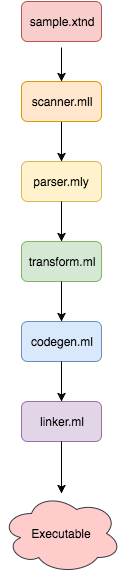
\includegraphics[width=.20\textwidth, height=15cm]{img/Execution.png}
\end{center}

\newpage

\section{The Extend Compiler}
The Extend compilation process consists of several source files, each of which performs a different function in the compilation pipeline.

\begin{itemize}
  \item \texttt{scanner.mll}: OCamllex scanner - consumes tokens.
  \item \texttt{parser.mly}: OCamlyacc parser - represents the Extend grammar.
  \item \texttt{ast.ml}: Abstract Syntax Tree, created from the output of the parser and representing the structure of an Extend program.
  \item \texttt{transform.ml}: Performs syntactic desugaring for easier compilation.
  \item \texttt{semant.ml}: Analyzes the semantics of the program to ensure that the program adheres to the rules of the language.
  \item \texttt{codegen.ml}: The LLVM IR code generator.
  \item \texttt{linker.ml}: Calls intermediary compilation steps on the generated \texttt{.ll}, including external functions if needed.
\end{itemize}

  \subsection{The Scanner}
  The function of \texttt{scanner.mll} is to parse a text stream into various tokens to be used in an Extend program.
  Only the tokens that are valid in Extend are to be given to the parser; all others will return a syntax error marked by the line and character number.

  \subsection{The Parser and Abstract Syntax Tree}
  The parser converts the tokens read by the scanner into a syntax tree deemed acceptable grammar within the Extend Language. This is converted into an Abstract Syntax Tree, which has nodes that can be consumed by the back end of the Extend compiler.

  \subsection{The Transformer}
The transformer is the first step in converting the AST into LLVM code. It takes the AST and reduces its breadth. This step is done to preserve the convenience for the user, but reduces the complexity for the actual compile step. A large number of internal variables are created in the process.

  \medskip \noindent This is how the user declares a variable.
  \begin{lstlisting}
    [2,2] foo;
  \end{lstlisting}

  \medskip \noindent This is how the transformer desugars the same code.
  \begin{lstlisting}
    rows_of_foo := 2;
    cols_of_foo := 2;
    [rows_of_foo, cols_of_foo] foo;
  \end{lstlisting}

  \medskip \noindent
  A similar transformation is performed on formula assignments:
  \begin{lstlisting}
    // Before Transformation:
    foo[g(x):4,3+3] = "Couldn't you have stuck to integers?";

    // After Transformation:
    start_row := g(x);
    end_row   := 4;
    start_col := 3+3;
    foo[start_row:end_row,start_col] = "Couldn't you have stuck to integers?";
  \end{lstlisting}
  \medskip \noindent
  Every expression on the left hand side before or after a comma or colon will become an internal temporary variable in the desugaring process. Internal variables are also created for the return expression and for any size assertions induced by the function signature:
  \begin{lstlisting}
    // Before Transformation:
    foo([m,n] arg1, [m, 1] arg2) {
      return m*n;
    }

    // After Transformation:
    foo(arg1, arg2) {
      m := numRows(arg1);
      n := numCols(arg1);
      asserts := (m == numRows(arg2)) && (1 == numCols(arg2));
      return_value := m*n;
      return return_value;
    }
  \end{lstlisting}
  In addition to generating temporary variables, Extend also transforms \texttt{\&\&, ||, and switch} into ternary conditionals to enable short-circuiting. Finally, the transformer performs some semantic analysis to ensure that there are no duplicate variables within a function, and no duplicate functions within a program.

  \subsection{The Semantic Analyzer}
  The semantic analyzer consumes the reduced AST. It ensures that Extend functions, variables, expressions, and more are being used properly at compile time, and throws flavorful exceptions to the user so that they may better understand why their program was illegal. In Extend, there are no real type errors involving expressions on the right-hand-side of a formula, as we attempt to degrade many gracefully. There are type errors possible on the left-hand side, but since they are assigned dynamically, very few can be determined at compile time. For function calls, the semantic analyzer ensures that the function exists and is called with the right number of arguments; and for variables, the analysis checks that the identifier refers to a real variables within the appropriate scope.

  \subsection{The Code Generator}
 Once the Extend AST passes semantic analysis, the code generator turns the reduced AST into LLVM code. Since the variable evaluation approach of Extend is not imperative, this process is fairly elaborate. There is one function created per formula, which is available to be called if the value of a cell with that formula is needed; and there is one function created per Extend function, which initializes a scope object with a collection of blueprints for all the local variables of that function. In its most basic form, each blueprint has a reference to one or more formulas that calculate the value of the variable. The section on the runtime goes into more detail on how this architecture is used.

  \subsection{The Linker}
  If successful LLVM IR is generated, the linker will adopt the role of building an executable object from the \texttt{.ll} file. This includes compiling it to an object file and linking the runtime environment along with other imported libraries.

  \section{Extend Runtime}
  Extend's cell values are lazily evaluated, which means they need to be implemented using function pointers. For each function that the Extend developer writes, the corresponding LLVM function that is generated is essentially identical: allocate a scope object for that function call, initialize that object with the appropriate set of variable definitions and the function arguments to that scope object, and then evaluate the variables corresponding to the size assertion and the return expression for that function. All of the "individualized" code lives in what we refer to as the formula-functions; for each distinct formula, the compiler generates a corresponding function that can be called when the corresponding cell's value is needed. Each formula-function shares the same signature: the arguments are a pointer to a scope and the row and column number of the cell being evaluated, and the return value is a pointer to a value struct (which holds the type and contents of the value.)

  The two main functions of our C runtime, therefore, are instantiate\_variable(), which looks at the variable definition "blueprint" and calculates the actual dimensions of the variable for that particular function call, and calculates the actual range of cells to which each formula applies; and getVal(), which determines if a particular cell value has already been calculated or not, and calls the appropriate formula-function if not.

  Before actually calling the main Extend entry point, our executable initializes a global array with the appropriate variable definitions for each function. When an Extend function is called, it simply copies the appropriate pointer into that array into its scope object.

  Leaving aside the variables introduced by the transformation step, this Extend function:
  \begin{lstlisting}
    foo() {
      x := 1;
      return x;
    }
  \end{lstlisting}
  \medskip \noindent
  would result in the LLVM equivalent of the following pseudocode (not written in any actual language) being generated:

  \begin{lstlisting}
    value_p foo() {
      scope = new ExtendScope;

      // Load the apropriate set of definitions for foo
      scope->defns = global_definitions[42];

      // Create an array of pointers to variable instances; one
      // pointer per variable. Only one variable in this function
      scope->insts = new var_instance* [1];

      // getVar calls instantiate_var if that instance pointer is still NULL,
      // or just returns the pointer if it's already been instantiated.
      // The instantiated variable keeps a copy of the pointer to its scope
      var_instance *return_variable = getVar(scope, 0);

      // Get the value of cell [0,0] of return_variable
      return getVal(return_variable, 0, 0);
    }
  \end{lstlisting}
  \medskip \noindent

  Since the newly initialized scope object will hold all NULL pointers for the instances, getVar() will end up calling instantiate\_variable, which will  determine that x has 1 row and 1 column; there is only a single formula for x, applying to all cells of x; and that that formula corresponds to the function pointer indicated in the variable definition.
  When getVal is called, the value pointer for the [0,0]th cell will similarly be NULL. As a result, getVal() will determine the function pointer for the appropriate formula and then call it, supplying as arguments a pointer to the scope and (0,0) for the row and column.

  The actual C structures used are listed below:
  \begin{lstlisting}

  // Each formula-function has the following signature:
  typedef value_p (*FormulaFP) (struct ExtendScope *scope, int row, int col);

  // This structure tells the runtime how to actually calculate the range of
  // cells to which each formula applies.
  struct ExtendFormula {
    /* These 10 variables correspond to formula_row_start through formula_col_end,
     * where char singleRow/Col are true if formula_row_end is None */
    char fromFirstRow;
    int rowStart_varnum;
    char toLastRow;
    int rowEnd_varnum;
    char fromFirstCol;
    int colStart_varnum;
    char toLastCol;
    int colEnd_varnum;

  	char isSingleRow;
  	char isSingleCol;

    FormulaFP formula;
  };

  // For a particular variable instance, this structure holds the results
  // of the calculations for each formula.
  struct ResolvedFormula {
  	int rowStart, rowEnd, colStart, colEnd;
  	FormulaFP formula;
  };

  struct var_defn {
    /* This is like a class definition - for every declared variable in the
     * Extend source, there should be one instance of these per compiled program.
     * They should just live in the global program storage.
     * It corresponds to Ast.variable */
     int rows_varnum;
     int cols_varnum;
     int numFormulas;
     struct ExtendFormula *formulas;
  	 char isOneByOne;
  	 char *name;
  };

  struct var_instance {
    /* This is an actual instance of a variable - we get one of these
     * per variable per time a function is called (assuming the contents
     * of the variable get examined.  */
  	int rows, cols;
  	int numFormulas;
  	struct ResolvedFormula *formulas;
    struct ExtendScope *closure;
    value_p *values;
  	char *status;
  	char *name;
  };

  // One scope object gets created per Extend function call
  struct ExtendScope {
    struct var_defn *defns;
    struct var_instance **vars;
  	int numVars;
  	int refcount;
  	value_p *functionParams;
  };
  \end{lstlisting}

  %\chapter{Testing}
Due to Extend being a large undertaking, we took steps to ensure that all features were working as the design of the language intended.

\medskip \noindent
This was done through implementing test cases that isolated specific aspects of the Extend language to ensure that each feature worked correctly. For basic components, we wrote a plethora of tests to illustrate functionality. For undertakings that required more debate on the design of the language, other tests were created and modified throughout development.

\section{Feature Integration \& Testing}
Development of new features naturally means that they must be deemed legal by the scanner, parser, semantic analyzer, and code generator. As we developed new features, the process was roughly as follows:
  \begin{enumerate}
    \item Write a simple test that illustrated the feature to test.
    \item Write the expected output of the aforementioned test to a text file.
    \item Confirm that the scanner consumes the tokens related to the feature.
    \item Confirm that the parser grammar has been adjusted to accomodate the new feature.
    \item Confirm that the semantic analyzer and transformer can properly identify and check the new feature code.
    \item Confirm that code generation generates the appropriate LLVM IR for the new features - such as allocating memory, building calls, and more.
    \item Ensure that the test written can write its output to stdout, to be compared with expected output.
    \item Compile and test the code to ensure that the code has worked to the team's expectations.
  \end{enumerate}

  \medskip \noindent
  Earlier in the development process, we tested the front end of our compiler by JSON-ifying the abstract syntax tree and examinining it. As we settled into full-fledged development, we would test with a full-feature regression test suite.

\section{Regression Test Suite}
Extend's regression test suite is executable through the \texttt{testscript.sh} script at the top level of the project. There are over 100 integration test files for various features of the Extend language, and a corresponding file with their expected output to \texttt{stdout}. This is to ensure that the successful implementation of one feature does not impact that of others.

\medskip \noindent
The test script iterates through every test file in the \texttt{inputs\_regression} directory. It compiles and executes the test, and compares it with the corresponding expected output file living in the \texttt{expected} directory. Some of these tests were "passing" tests, meant to confirm successful output, and some were "failing" tests, identifying the ability of the language to detect illegal actions and exit gracefully.

\medskip \noindent
\textbf{Note:} We have added a full test listing at the end of this document. Please refer to the chapter titled "Test Listing" for more detail.

  \subsection{Integration with Travis CI}
  The aforementioned test suite is run by Travis CI in the event that the Extend compiler is successfully built; otherwise, the build will fail and exit. In our development workflow, checking the logs during build failures sometimes revealed that tests in the regression test suite did not succeed as expected. This integration kept the far-reaching effects of newly introduced features entirely transparent throughout the process.

  %\input{tex/lessons}
  \chapter{Extend Code Listing}
\section{scanner.mll}
\begin{lstlisting}{ocaml}
{
  open Lexing
  open Parser
  open String

  exception SyntaxError of string
  let syntax_error lexbuf = raise (SyntaxError("Invalid character: " ^ Lexing.lexeme lexbuf))
}

let digit = ['0'-'9']
let exp = 'e'('+'|'-')?['0'-'9']+
let flt = (digit)+ ('.' (digit)* exp?|exp)
let id = ['a'-'z' 'A'-'Z']['a'-'z' 'A'-'Z' '0'-'9' '_']*


rule token = parse
  ['\n']               { new_line lexbuf; token lexbuf }
| [' ' '\t' '\r']      { token lexbuf }   (* Whitespace *)
| "/*"                 { multiline_comment lexbuf }
| "//"                 { oneline_comment lexbuf }
| '"'                  { read_string (Buffer.create 17) lexbuf }
| '['             { LSQBRACK }
| ']'             { RSQBRACK }
| '('             { LPAREN }
| ')'             { RPAREN }
| '{'             { LBRACE }
| '}'             { RBRACE }
| ":="            { GETS }
| '='             { ASN }
| ':'             { COLON }
| ','             { COMMA }
| "->"            { PRECEDES }
| '?'             { QUESTION }
| "=="            { EQ }
| "!="            { NOTEQ }
| '<'             { LT }
| '>'             { GT }
| "<="            { LTEQ }
| ">="            { GTEQ }
| ';'             { SEMI }
| '!'             { LOGNOT }
| "&&"            { LOGAND }
| "||"            { LOGOR }
| '~'             { BITNOT }
| '&'             { BITAND }
| '|'             { BITOR }
| '^'             { BITXOR }
| '+'             { PLUS }
| '-'             { MINUS }
| '*'             { TIMES }
| '/'             { DIVIDE }
| '%'             { MOD }
| "**"            { POWER }
| "<<"            { LSHIFT }
| ">>"            { RSHIFT }
| '#'             { HASH }
| "if"            { IF }
| "empty"         { EMPTY }
| "size"          { SIZE }
| "typeof"        { TYPEOF }
| "row"           { ROW }
| "column"        { COLUMN }
| "switch"        { SWITCH }
| "case"          { CASE }
| "default"       { DEFAULT }
| "return"        { RETURN }
| "import"        { IMPORT }
| "global"        { GLOBAL }
| "extern"        { EXTERN }
| digit+ as lit   { LIT_INT(int_of_string lit) }
| flt as lit      { LIT_FLOAT(float_of_string lit) }
| id as lit       { ID(lit) }
| eof             { EOF }
| _               { syntax_error lexbuf }

and multiline_comment = parse
  "*/" { token lexbuf }
| '\n' { new_line lexbuf; multiline_comment lexbuf }
| _    { multiline_comment lexbuf }

and oneline_comment = parse
  '\n' { new_line lexbuf; token lexbuf }
| _    { oneline_comment lexbuf }

(* read_string mostly taken from:
https://realworldocaml.org/v1/en/html/parsing-with-ocamllex-and-menhir.html *)
and read_string buf =
  parse
  | '"'       { LIT_STRING (Buffer.contents buf) }
  | '\n'      { new_line lexbuf; Buffer.add_char buf '\n'; read_string buf lexbuf }
  | '\\' 'n'  { Buffer.add_char buf '\n'; read_string buf lexbuf }
  | '\\' 'r'  { Buffer.add_char buf '\r'; read_string buf lexbuf }
  | '\\' 't'  { Buffer.add_char buf '\t'; read_string buf lexbuf }
  | '\\' ([^'\\' 'n' 'r' 't'] as lxm)
    { Buffer.add_char buf lxm; read_string buf lexbuf }
  | [^ '"' '\\']+
    { Buffer.add_string buf (Lexing.lexeme lexbuf);
      read_string buf lexbuf
    }
  | _         { syntax_error lexbuf }
  | eof       { raise (Failure("unterminated string")) }
\end{lstlisting}
\section{parser.mly}
\begin{lstlisting}{ocaml}
/* Ocamlyacc parser for Extend */

%{
open Ast
%}

%token LSQBRACK RSQBRACK LPAREN RPAREN LBRACE RBRACE HASH
%token COLON COMMA QUESTION IF GETS ASN SEMI PRECEDES
%token SWITCH CASE DEFAULT SIZE TYPEOF ROW COLUMN
%token PLUS MINUS TIMES DIVIDE MOD POWER LSHIFT RSHIFT
%token EQ NOTEQ GT LT GTEQ LTEQ
%token LOGNOT LOGAND LOGOR
%token BITNOT BITXOR BITAND BITOR
%token EMPTY RETURN IMPORT GLOBAL EXTERN
%token <int> LIT_INT
%token <float> LIT_FLOAT
%token <string> LIT_STRING
%token <string> ID
%token EOF

%right QUESTION
%left PRECEDES
%left LOGOR
%left LOGAND
%left EQ NOTEQ LT GT LTEQ GTEQ
%left PLUS MINUS BITOR BITXOR
%left TIMES DIVIDE MOD LSHIFT RSHIFT BITAND
%right POWER
%right BITNOT LOGNOT NEG
%left LSQBRACK

%start program
%type <Ast.raw_program> program

%%

program:
    program_piece EOF {  let (imp, glob, fnc, ext) = $1 in (List.rev imp, List.rev glob, List.rev fnc, List.rev ext) }

program_piece:
    /* nothing */ {([],[],[],[])}
  | program_piece import      { let (imp, glob, fnc, ext) = $1 in ($2 :: imp, glob, fnc, ext) }
  | program_piece global      { let (imp, glob, fnc, ext) = $1 in (imp, $2 :: glob, fnc, ext) }
  | program_piece func_decl   { let (imp, glob, fnc, ext) = $1 in (imp, glob, $2 :: fnc, ext) }
  | program_piece extern      { let (imp, glob, fnc, ext) = $1 in (imp, glob, fnc, $2 :: ext) }

import:
    IMPORT LIT_STRING SEMI {$2}

global:
    GLOBAL varinit {$2}

extern:
    EXTERN LIT_STRING LBRACE opt_extern_list RBRACE {(Library($2, $4))}

opt_extern_list:
    /* nothing */ { [] }
  | extern_list { List.rev $1 }

extern_list:
    extern_fn { [$1] }
  | extern_list extern_fn { $2 :: $1 }

extern_fn:
    ID LPAREN func_param_list RPAREN SEMI
    { {
      extern_fn_name = $1;
      extern_fn_params = $3;
      extern_fn_libname = "";
      extern_ret_val = (None, None);
    } }

func_decl:
    ID LPAREN func_param_list RPAREN LBRACE opt_stmt_list ret_stmt RBRACE
    { {
      name = $1;
      params = $3;
      body = $6;
      raw_asserts = [];
      ret_val = ((None, None), $7)
    } }

opt_stmt_list:
    /* nothing */ { [] }
  | stmt_list { List.rev $1 }

stmt_list:
    stmt { [$1] }
  | stmt_list stmt { $2 :: $1 }

stmt:
    varinit { $1 } |  assign { $1 }

ret_stmt:
    RETURN expr SEMI {$2}

varinit:
    var_list SEMI { Varinit((None, None), List.rev $1) }
  | dim var_list SEMI { Varinit($1, List.rev $2) }

var_list:
    ID varassign { [ ($1, $2)] }
  | var_list COMMA ID varassign { ($3, $4) :: $1}

varassign:
    /* nothing */ { None }
  | GETS expr { Some $2 }

assign:
    ID lhs_sel ASN expr SEMI { Assign($1, $2, Some $4) }

expr:
    expr rhs_sel        { Selection($1, $2) }
  | HASH ID             { Selection(Id($2), (None, None)) }
  | op_expr             { $1 }
  | ternary_expr        { $1 }
  | switch_expr         { $1 }
  | func_expr           { $1 }
  | range_expr          { $1 }
  | expr PRECEDES expr  { Precedence($1, $3) }
  | LPAREN expr RPAREN  { $2 }
  | ID                  { Id($1) }
  | LIT_INT             { LitInt($1) }
  | LIT_FLOAT           { LitFlt($1) }
  | LIT_STRING          { LitString($1) }
  | EMPTY               { Empty }

op_expr:
    expr PLUS expr      { BinOp($1, Plus, $3) }
  | expr MINUS expr     { BinOp($1, Minus, $3) }
  | expr TIMES expr     { BinOp($1, Times, $3) }
  | expr DIVIDE expr    { BinOp($1, Divide, $3) }
  | expr MOD expr       { BinOp($1, Mod, $3) }
  | expr POWER expr     { BinOp($1, Pow, $3) }
  | expr LSHIFT expr    { BinOp($1, LShift, $3) }
  | expr RSHIFT expr    { BinOp($1, RShift, $3) }
  | expr LOGAND expr    { BinOp($1, LogAnd, $3) }
  | expr LOGOR expr     { BinOp($1, LogOr, $3) }
  | expr BITXOR expr    { BinOp($1, BitXor, $3) }
  | expr BITAND expr    { BinOp($1, BitAnd, $3) }
  | expr BITOR expr     { BinOp($1, BitOr, $3) }
  | expr EQ expr        { BinOp($1, Eq, $3) }
  | expr NOTEQ expr     { UnOp(LogNot,(BinOp($1, Eq, $3))) }
  | expr GT expr        { BinOp($1, Gt, $3) }
  | expr LT expr        { BinOp($1, Lt, $3) }
  | expr GTEQ expr      { BinOp($1, GtEq, $3) }
  | expr LTEQ expr      { BinOp($1, LtEq, $3) }
  | SIZE LPAREN expr RPAREN { UnOp(SizeOf, $3) }
  | TYPEOF LPAREN expr RPAREN { UnOp(TypeOf, $3) }
  | ROW LPAREN RPAREN       { UnOp(Row, Empty)}
  | COLUMN LPAREN RPAREN    { UnOp(Column, Empty)}
  | MINUS expr %prec NEG    { UnOp(Neg, $2) }
  | LOGNOT expr             { UnOp(LogNot, $2) }
  | BITNOT expr             { UnOp(BitNot, $2) }

ternary_expr:
    IF LPAREN expr COMMA expr COMMA expr RPAREN { Ternary($3, $5, $7) }
  | expr QUESTION expr COLON expr %prec QUESTION { Ternary($1, $3, $5) }

switch_expr:
    SWITCH LPAREN switch_cond RPAREN LBRACE default_case_list RBRACE { Switch($3, fst $6, snd $6) }
  | SWITCH LBRACE default_case_list RBRACE { Switch(None, fst $3, snd $3) }

switch_cond:
    /* nothing */ { None }
  | expr { Some $1 }

default_case_list:
    case_list {(List.rev $1, Empty)}
  | case_list default_expr {(List.rev $1, $2)}

case_list:
    case_stmt { [$1] }
  | case_list case_stmt { $2 :: $1 }

case_stmt:
    CASE case_expr_list COLON expr SEMI { (List.rev $2, $4) }

default_expr:
    DEFAULT COLON expr SEMI { $3 }

case_expr_list:
    expr { [$1] }
  | case_expr_list COMMA expr { $3 :: $1 }

func_expr:
    ID LPAREN opt_arg_list RPAREN { Call($1, $3) }

range_expr:
    LBRACE row_list RBRACE { allow_range_literal (LitRange(List.rev $2)) }

row_list:
    col_list {[List.rev $1]}
  | row_list SEMI col_list {List.rev $3 :: $1}

col_list:
    expr {[$1]}
  | col_list COMMA expr {$3 :: $1}

opt_arg_list:
    /* nothing */ {[]}
  | arg_list { List.rev $1 }

arg_list:
    expr {[$1]}
  | arg_list COMMA expr {$3 :: $1}

lhs_sel:
    /* nothing */                         { (None, None) }
/* commented out: LSQBRACK lslice RSQBRACK { (Some $2, None) } */
  | LSQBRACK lslice COMMA lslice RSQBRACK { (Some $2, Some $4) }

rhs_sel:
    LSQBRACK rslice RSQBRACK              { (Some $2, None) }
  | LSQBRACK rslice COMMA rslice RSQBRACK { (Some $2, Some $4) }

lslice:
  /* commented out: nothing production { (None, None) } */
    lslice_val                            { (Some $1, None) }
  | lslice_val COLON lslice_val           { (Some $1, Some $3) }
  | lslice_val COLON                      { (Some $1, Some DimensionEnd) }
  | COLON lslice_val                      { (Some DimensionStart, Some $2) }
  | COLON                                 { (Some DimensionStart, Some DimensionEnd) }

rslice:
    /* nothing */                         { (None, None) }
  | rslice_val                            { (Some $1, None) }
  | rslice_val COLON rslice_val           { (Some $1, Some $3) }
  | rslice_val COLON                      { (Some $1, Some DimensionEnd) }
  | COLON rslice_val                      { (Some DimensionStart, Some $2) }
  | COLON                                 { (Some DimensionStart, Some DimensionEnd) }

lslice_val:
    expr { Abs($1) }

rslice_val:
    expr { Abs($1) }
  | LSQBRACK expr RSQBRACK { Rel($2) }

func_param_list:
    /* nothing */ { [] }
  | func_param_int_list { List.rev $1 }

func_param_int_list:
    func_sin_param { [$1] }
  | func_param_int_list COMMA func_sin_param { $3 :: $1 }

func_sin_param:
    ID { ((None, None), $1) }
  | dim ID { ($1, $2) }

dim:
    LSQBRACK expr RSQBRACK { (Some $2, None) }
  | LSQBRACK expr COMMA expr RSQBRACK { (Some $2, Some $4) }
\end{lstlisting}
\section{ast.ml}
\begin{lstlisting}{ocaml}
type op       = Plus | Minus | Times | Divide | Mod | Pow |
                LShift | RShift | BitOr | BitAnd | BitXor |
                Eq | Gt | GtEq | Lt | LtEq | LogAnd | LogOr
type unop     = Neg | LogNot | BitNot | SizeOf | TypeOf | Row | Column | Truthy

type expr     = LitInt of int |
                LitFlt of float |
                LitString of string |
                LitRange of (expr list) list |
                Id of string |
                Empty |
                BinOp of expr * op * expr |
                UnOp of unop * expr |
                Ternary of expr * expr * expr |
                Switch of expr option * case list * expr |
                Call of string * expr list |
                Selection of expr * sel |
                ReducedTernary of string * string * string |
                Precedence of expr * expr
and  index    = Abs of expr |
                Rel of expr |
                DimensionStart |
                DimensionEnd
and  slice    = index option * index option
and  sel      = slice option * slice option
and  case     = expr list * expr

type dim      = expr option * expr option
type var      = dim * string
type assign   = string * sel * expr option
type init     = string * expr option
type stmt     = Assign of assign |
                Varinit of dim * init list

type raw_func = {
    name: string;
    params: var list;
    body: stmt list;
    raw_asserts: expr list;
    ret_val: dim * expr;
}

type extern_func = {
    extern_fn_name: string;
    extern_fn_params: var list;
    extern_fn_libname: string;
    extern_ret_val: dim;
}

type library  = Library of string * extern_func list
type raw_program = string list * stmt list * raw_func list * library list

(* Desugared types below *)
module StringMap = Map.Make(String)
type formula  = {
  formula_row_start: index;
  formula_row_end: index option;
  formula_col_start: index;
  formula_col_end: index option;
  formula_expr: expr;
}

type dim_expr = DimOneByOne
              | DimId of string

type variable = {
  var_rows: dim_expr;
  var_cols: dim_expr;
  var_formulas: formula list;
}

type func_decl = {
  func_params: var list;
  func_body: variable StringMap.t;
  func_asserts: expr list;
  func_ret_val: dim * expr;
}

type program = (variable StringMap.t) * (func_decl StringMap.t) * (extern_func StringMap.t)

type listable = Inits of init list |
                Vars of var list |
                Stmts of stmt list |
                RawFuncs of raw_func list |
                Externs of extern_func list |
                Libraries of library list |
                Exprs of expr list |
                Rows of (expr list) list |
                Strings of string list |
                Cases of case list |
                Formulas of formula list

exception IllegalRangeLiteral of string
exception TransformedAway of string

let quote_string str =
  let escape_characters = Str.regexp "[\n \t \r \\ \"]" in
  let replace_fn s = match Str.matched_string s with
    "\n" -> "\\n"   |
    "\t" -> "\\t"   |
    "\r" -> "\\r"   |
    "\\" -> "\\\\"  |
    "\"" -> "\\\""  |
    _    -> Str.matched_string s in
  "\"" ^ Str.global_substitute escape_characters replace_fn str ^ "\""

let string_of_op o = "\"" ^ (match o with
    Plus -> "+" | Minus -> "-" | Times -> "*" | Divide -> "/" | Mod -> "%" | Pow -> "**" |
    LShift -> "<<" | RShift -> ">>" | BitOr -> "|" | BitAnd -> "&" | BitXor -> "^" |
    Eq -> "==" | Gt -> ">" | GtEq -> ">=" | Lt -> "<" | LtEq -> "<=" |
    LogAnd -> "&& " | LogOr -> "||" ) ^ "\""

let string_of_unop = function
    Neg -> "\"-\"" | LogNot -> "\"!\"" | BitNot -> "\"~\"" | Truthy -> "\"truthy\"" |
    SizeOf -> "\"size\"" | TypeOf -> "\"type\"" | Row -> "\"row\"" | Column -> "\"column\""

let rec string_of_expr = function
    LitInt(l) ->          "{\"LitInt\":" ^ string_of_int l ^ "}"
  | LitFlt(l) ->          "{\"LitFlt\":" ^ string_of_float l ^ "}"
  | LitString(s) ->       "{\"LitString\":" ^ quote_string s ^ "}"
  | LitRange(rowlist) ->  "{\"LitRange\": " ^ string_of_list (Rows rowlist) ^ "}"
  | Id(s) ->              "{\"Id\": " ^ quote_string s ^ "}"
  | Empty ->              "\"Empty\""
  | BinOp(e1, o, e2) ->   "{\"BinOp\": {" ^
                            "\"expr1\": " ^ string_of_expr e1 ^ ", " ^
                            "\"operator\": " ^ string_of_op o ^ ", " ^
                            "\"expr2\": " ^ string_of_expr e2 ^ "}}"
  | UnOp(o, e) ->         "{\"UnOp\": {" ^
                            "\"operator\": " ^ string_of_unop o ^ ", " ^
                            "\"expr\": " ^ string_of_expr e ^ "}}"
  | Ternary(c, e1, e2) -> "{\"Ternary\": {" ^
                            "\"condition\": " ^ string_of_expr c ^ ", " ^
                            "\"ifExpr\": " ^ string_of_expr e1 ^ ", " ^
                          "\"elseExpr\": " ^ string_of_expr e2 ^ "}}"
  | ReducedTernary(s1, s2, s3) -> "{\"ReducedTernary\": {" ^
                            "\"truthiness\": " ^ quote_string s1 ^ ", " ^
                            "\"true_values\": " ^ quote_string s2 ^ ", " ^
                            "\"false_values\": " ^ quote_string s3 ^ "}}"
  | Switch(eo, cases, dflt) ->  "{\"Switch\": {" ^
                                "\"condition\": " ^
                                  (match eo with None -> "null" | Some e -> string_of_expr e) ^ ", " ^
                                "\"cases\": " ^ string_of_list (Cases cases) ^ ", " ^
                                "\"defaultExpr\": " ^ string_of_expr dflt ^ "}}"
  | Call(f, arguments) -> "{\"Call\": {" ^
                            "\"function\": " ^ quote_string f ^ ", " ^
                            "\"arguments\": " ^ string_of_list (Exprs arguments) ^ "}}"
  | Selection(e, s) ->    "{\"Selection\": {" ^
                            "\"expr\": " ^ string_of_expr e ^ ", " ^
                            "\"slices\": " ^ string_of_sel s ^ "}}"
  | Precedence(e1, e2) -> "{\"Precedence\": { " ^
                            "\"prior_expr\": " ^ string_of_expr e1 ^ ", " ^
                          "\"dependent_expr\": " ^ string_of_expr e2 ^ "}}"

and string_of_case (el, e) =
    "{\"Cases\": " ^ string_of_list (Exprs el) ^ ", " ^
     "\"expr\": " ^ string_of_expr e ^ "}"

and string_of_sel (s1, s2) =
    "{\"slice1\": " ^ string_of_slice s1 ^ ", \"slice2\": " ^ string_of_slice s2 ^ "}"

and string_of_slice = function
    None -> "null"
  | Some (start_idx, end_idx) -> "{\"start\": " ^ string_of_index start_idx ^ ", \"end\": " ^ string_of_index end_idx ^ "}"

and string_of_index = function
    None -> "null"
  | Some(Abs(e)) -> "{\"Absolute\": " ^ string_of_expr e ^ "}"
  | Some(Rel(e)) -> "{\"Relative\": " ^ string_of_expr e ^ "}"
  | Some(DimensionStart) -> "\"DimensionStart\""
  | Some(DimensionEnd) -> "\"DimensionEnd\""

and string_of_dim (d1,d2) = "{\"d1\": " ^ (match d1 with None -> "null" | Some e -> string_of_expr e) ^ ", " ^
                             "\"d2\": " ^ (match d2 with None -> "null" | Some e -> string_of_expr e) ^ "}"

and string_of_var (d, s) = "{\"Dimensions\": " ^ string_of_dim d ^ ", " ^
                            "\"VarName\": " ^ quote_string s ^ "}"

and string_of_assign (s, selection, eo) =
    "{\"VarName\": " ^ quote_string s ^ ", " ^
     "\"Selection\": " ^ string_of_sel selection ^ ", " ^
    "\"expr\": " ^ (match eo with None -> "null" | Some e -> string_of_expr e) ^ "}"

and string_of_varinit (d, inits) =
  "{\"Dimensions\": " ^ string_of_dim d ^
    ",\"Initializations\": " ^ string_of_list (Inits inits) ^ "}"

and string_of_init (s, eo) =
    "{\"VarName\": " ^ quote_string s ^ ", " ^
     "\"expr\": " ^ (match eo with None -> "null" | Some e -> string_of_expr e) ^ "}"

and string_of_stmt = function
    Assign(a) -> "{\"Assign\": " ^ string_of_assign a ^ "}"
  | Varinit(d, inits) -> "{\"Varinit\": " ^ string_of_varinit (d, inits) ^ "}"

and string_of_range (d, e) = "{\"Dimensions\": " ^ string_of_dim d ^ ", " ^
                              "\"expr\": " ^ string_of_expr e ^ "}"

and string_of_raw_func fd =
    "{\"Name\": " ^ quote_string fd.name ^ "," ^
     "\"Params\": " ^ string_of_list (Vars fd.params) ^ "," ^
     "\"Stmts\": " ^ string_of_list (Stmts fd.body) ^ "," ^
     "\"Assertions\": " ^ string_of_list (Exprs fd.raw_asserts) ^ "," ^
     "\"ReturnVal\": " ^ string_of_range fd.ret_val ^ "}"

and string_of_extern_func fd =
  "{\"Name\": " ^ quote_string fd.extern_fn_name ^ "," ^
  "\"Params\": " ^ string_of_list (Vars fd.extern_fn_params) ^ "," ^
  "\"Library\": " ^ quote_string fd.extern_fn_libname ^ "," ^
  "\"ReturnDim\": " ^ string_of_dim fd.extern_ret_val ^ "}"

and string_of_library (Library(lib_name, lib_fns)) =
  "{\"LibraryName\": " ^ quote_string lib_name ^ "," ^
  "\"ExternalFunctions\": " ^ string_of_list (Externs lib_fns) ^ "}"

and string_of_dimexpr = function
    DimOneByOne -> "1"
  | DimId(s) -> quote_string s

and string_of_formula f =
  "{\"RowStart\": " ^ string_of_index (Some f.formula_row_start) ^ "," ^
  "\"RowEnd\": " ^ string_of_index (f.formula_row_end) ^ "," ^
  "\"ColumnStart\": " ^ string_of_index (Some f.formula_col_start) ^ "," ^
  "\"ColumnEnd\": " ^ string_of_index (f.formula_col_end) ^ "," ^
  "\"Formula\": " ^ string_of_expr f.formula_expr ^ "}"

and string_of_list l =
  let stringrep = (match l with
    Inits (il) -> List.map string_of_init il
  | Vars(vl) -> List.map string_of_var vl
  | Stmts(sl) -> List.map string_of_stmt sl
  | RawFuncs(fl) -> List.map string_of_raw_func fl
  | Externs(efl) -> List.map string_of_extern_func efl
  | Libraries(libl) -> List.map string_of_library libl
  | Exprs(el) -> List.map string_of_expr el
  | Rows(rl) -> List.map (fun (el : expr list) -> string_of_list (Exprs el)) rl
  | Strings(sl) -> List.map quote_string sl
  | Cases(cl) -> List.map string_of_case cl
  | Formulas(fl) -> List.map string_of_formula fl)
  in "[" ^ String.concat ", " stringrep ^ "]"

let string_of_raw_program (imp, glb, fs, exts) =
    "{\"Program\": {" ^
      "\"Imports\": " ^ string_of_list (Strings imp) ^ "," ^
      "\"Globals\": " ^ string_of_list (Stmts glb) ^ "," ^
      "\"ExternalLibraries\": " ^ string_of_list (Libraries exts) ^ "," ^
      "\"Functions\": " ^ string_of_list (RawFuncs fs) ^ "}}"

let string_of_variable v =
  "{\"Rows\": " ^ string_of_dimexpr v.var_rows ^ "," ^
  "\"Columns\": " ^ string_of_dimexpr v.var_cols ^ "," ^
  "\"Formulas\": " ^ string_of_list (Formulas v.var_formulas) ^ "}"

let string_of_map value_desc val_printing_fn m =
  let f_key_val_list k v l = (
    "{\"" ^ value_desc ^ "Name\": " ^ quote_string k ^ ", " ^
    "\"" ^ value_desc ^ "Def\": " ^ val_printing_fn v ^ "}"
  ) :: l in
  "[" ^ String.concat ", " (List.rev (StringMap.fold f_key_val_list m [])) ^ "]"

let string_of_funcdecl f =
  "{\"Params\": " ^ string_of_list (Vars f.func_params) ^ "," ^
  "\"Variables\": " ^ string_of_map "Variable" string_of_variable f.func_body ^ "," ^
  "\"Assertions\": " ^ string_of_list (Exprs f.func_asserts) ^ "," ^
  "\"ReturnVal\": " ^ string_of_range f.func_ret_val ^ "}"

let string_of_program (glb, fs, exts) =
  "{\"Program\": {" ^
    "\"Globals\": " ^ string_of_map "Variable" string_of_variable glb ^ "," ^
    "\"Functions\": " ^ string_of_map "Function" string_of_funcdecl fs ^ "," ^
    "\"ExternalFunctions\": " ^ string_of_map "ExternalFunctions" string_of_extern_func exts ^ "}}"

let allow_range_literal = function
    LitRange(rowlist) ->
      let rec check_range_literal rl =
        List.for_all (fun exprs -> List.for_all check_basic_expr exprs) rl
      and check_basic_expr = function
          LitInt(_) | UnOp(Neg, LitInt(_)) | LitFlt(_) | UnOp(Neg, LitFlt(_)) | LitString(_) | Empty -> true
        | LitRange(rl) -> check_range_literal rl
        | _ -> false in

      if check_range_literal rowlist then LitRange(rowlist)
      else raise(IllegalRangeLiteral(string_of_expr (LitRange(rowlist))))
  | e -> raise(IllegalRangeLiteral(string_of_expr e))
\end{lstlisting}
\section{transform.ml}
\begin{lstlisting}{ocaml}
open Ast
open Lexing
open Parsing
open Semant

module StringSet = Set.Make (String);;
let importSet = StringSet.empty;;

let idgen =
  (* from http://stackoverflow.com/questions/10459363/side-effects-and-top-level-expressions-in-ocaml*)
  let count = ref (-1) in
  fun prefix -> incr count; "_tmp_" ^ prefix ^ string_of_int !count;;

let expand_file include_stdlib filename =
  let print_error_location filename msg lexbuf =
    let pos = lexbuf.lex_curr_p in
    prerr_endline ("Syntax error in \"" ^ filename ^ "\": " ^ msg) ;
    prerr_endline ("Line " ^ (string_of_int pos.pos_lnum) ^ " at character " ^ (string_of_int (pos.pos_cnum - pos.pos_bol))) in

  let rec expand_imports processed_imports globals fns exts dir = function
      [] -> ([], globals, fns, exts)
    | (import, use_dir) :: imports ->
      (* print_endline "--------";
      print_endline ("Working on: " ^ import) ;
      print_endline ("Already processed:"); *)
      (* StringSet.iter (fun a -> print_endline a) processed_imports; *)
      let in_chan = open_in import in
      let lexbuf = (Lexing.from_channel (in_chan)) in
      let (file_imports, file_globals, file_functions, file_externs) =
        try Parser.program Scanner.token lexbuf
        with
          Parsing.Parse_error -> print_error_location import "" lexbuf ; exit(-1)
        | Scanner.SyntaxError(s) -> print_error_location import s lexbuf ; exit(-1)
      in
      let file_imports = List.map (fun file -> (if use_dir then (dir ^ "/") else "") ^ file) file_imports in
      let new_proc = StringSet.add import processed_imports and _ = close_in in_chan in
      (* print_endline ("Now I'm done with: ") ; *)
      (* StringSet.iter (fun a -> print_endline a) new_proc; *)
      let first_im_hearing_about imp = not (StringSet.mem imp new_proc || List.mem imp (List.map fst imports)) in
      let new_imports = List.map (fun e -> (e, true)) (StringSet.elements (StringSet.of_list (List.filter first_im_hearing_about file_imports))) in
      (* print_endline ("First I'm hearing about:") ; *)
      (* List.iter print_endline new_imports; *)
      expand_imports new_proc (globals @ file_globals) (fns @ file_functions) (exts @ file_externs) (Filename.dirname import) (imports @ new_imports) in
  expand_imports
    StringSet.empty [] [] []
    (Filename.dirname filename)
    (if include_stdlib then [(filename, true); ("src/stdlib/stdlib.xtnd", false)] else [(filename, true)])

let expand_expressions (imports, globals, functions, externs) =
  let lit_zero = LitInt(0) in let abs_zero = Abs(lit_zero) in
  let lit_one  = LitInt(1) in let abs_one  = Abs(lit_one)  in
  let one_by_one = (Some lit_one, Some lit_one) in
  let zero_comma_zero = (Some (Some abs_zero, Some abs_one),
                         Some (Some abs_zero, Some abs_one)) in
  let entire_dimension = (Some DimensionStart, Some DimensionEnd) in
  let entire_range = (Some entire_dimension, Some entire_dimension) in

  let expand_expr expr_loc = function
    (* Create a new variable for all expressions on the LHS to hold the result;
       return the new expression and whatever new statements are necessary to create the new variable *)
      Empty     -> raise (IllegalExpression("Empty not allowed in " ^ expr_loc))
    | LitString(s) -> raise (IllegalExpression("String literal " ^ quote_string s ^ " not allowed in " ^ expr_loc))
    | LitRange(rl) -> raise (IllegalExpression("Range literal " ^ string_of_list (Rows rl) ^ " not allowed in " ^ expr_loc))
    | e         -> let new_id = idgen expr_loc in (
        Id(new_id),
        [Varinit (one_by_one, [(new_id, None)]);
         Assign (new_id, zero_comma_zero, Some e)]) in

  let expand_index index_loc = function
    (* Expand one index of a slice if necessary. *)
      Abs(e) -> let (new_e, new_stmts) = expand_expr index_loc e in
      (Abs(new_e), new_stmts)
    | DimensionStart -> (DimensionStart, [])
    | DimensionEnd -> (DimensionEnd, [])
    | Rel(_) -> raise (IllegalExpression("relative - this shouldn't be possible")) in

  let expand_slice slice_loc = function
    (* Expand one or both sides as necessary. *)
      None -> (entire_dimension, [])
    | Some (Some (Abs(e)), None) ->
      let (start_e, start_stmts) = expand_expr (slice_loc ^ "_start") e in
      ((Some (Abs(start_e)), None), start_stmts)
    | Some (Some idx_start, Some idx_end) ->
      let (new_start, new_start_exprs) = expand_index (slice_loc ^ "_start") idx_start in
      let (new_end, new_end_exprs) = expand_index (slice_loc ^ "_end") idx_end in
      ((Some new_start, Some new_end), new_start_exprs @ new_end_exprs)
    | Some (Some _, None) | Some (None, _) -> raise (IllegalExpression("Illegal slice - this shouldn't be possible")) in

  let expand_assign asgn_loc (var_name, (row_slice, col_slice), formula) =
    (* expand_assign: Take an Assign and return a list of more
       atomic statements, with new variables replacing any
       complex expressions in the selection slices and with single
       index values desugared to expr:expr+1. *)
    try
      let (new_row_slice, row_exprs) = expand_slice (asgn_loc ^ "_" ^ var_name ^ "_row") row_slice in
      let (new_col_slice, col_exprs) = expand_slice (asgn_loc ^ "_" ^ var_name ^ "_col") col_slice in
      Assign(var_name, (Some new_row_slice, Some new_col_slice), formula) :: (row_exprs @ col_exprs)
    with IllegalExpression(s) ->
      raise (IllegalExpression("Illegal expression (" ^ s ^ ") in " ^
                               string_of_assign (var_name, (row_slice, col_slice), formula))) in

  let expand_init (r, c) (v, e) =
    Varinit((Some r, Some c), [(v, None)]) ::
    match e with
      None -> []
    | Some e -> [Assign (v, entire_range, Some e)] in

  let expand_dimension dim_loc = function
      None -> expand_expr dim_loc (LitInt(1))
    | Some e -> expand_expr dim_loc e in

  let expand_varinit fname ((row_dim, col_dim), inits) =
    (* expand_varinit: Take a Varinit and return a list of more atomic
       statements. Each dimension will be given a temporary ID, which
       will be declared as [1,1] _tmpXXX; the formula for tmpXXX will be
       set as a separate assignment; the original variable will be
       declared as [_tmpXXX, _tmpYYY] var; and the formula assignment
       will be applied to [:,:]. *)
    try
      let (row_e, row_stmts) = expand_dimension (fname ^ "_" ^ (String.concat "_" (List.map fst inits)) ^ "_row_dim") row_dim in
      let (col_e, col_stmts) = expand_dimension (fname ^ "_" ^ (String.concat "_" (List.map fst inits)) ^ "_col_dim") col_dim in
      row_stmts @ col_stmts @ List.concat (List.map (expand_init (row_e, col_e)) inits)
    with IllegalExpression(s) ->
      raise (IllegalExpression("Illegal expression (" ^ s ^ ") in " ^
                               string_of_varinit ((row_dim, col_dim), inits))) in

  let expand_stmt fname = function
    Assign(a) -> expand_assign fname a
  | Varinit(d, inits) -> expand_varinit fname (d, inits) in

  let expand_stmt_list fname stmts = List.concat (List.map (expand_stmt fname) stmts) in

  let expand_params fname params =
    let needs_sizevar = function
        ((None, None), _) -> false
      | _ -> true in
    let params_with_sizevar = List.map (fun x -> (idgen (fname ^ "_" ^ (snd x) ^ "_size"), x)) (List.filter needs_sizevar params) in
    let expanded_args = List.map (fun (sv, ((rv, cv), s)) -> ((sv, s), [((sv, abs_zero), rv); ((sv, abs_one), cv)])) params_with_sizevar in
    let (sizes, inits) = (List.map fst expanded_args, List.concat (List.map snd expanded_args)) in
    let add_item (varset, (assertlist, initlist)) ((sizevar, pos), var) =
      (match var with
         Some Id(s) ->
         if StringSet.mem s varset then
           (* We've seen this variable before; don't initialize it, just assert it *)
           (varset, (BinOp(Id(s), Eq, Selection(Id(sizevar), (Some(Some(pos), None), None))) :: assertlist, initlist))
         else
           (* We're seeing a string for the first time; don't assert it, just create it *)
           (StringSet.add s varset, (assertlist,
                                     Assign(s, zero_comma_zero, Some (Selection(Id(sizevar), (Some(Some(pos), None), None)))) ::
                                     Varinit(one_by_one, [(s, None)]) ::
                                     initlist))
       | Some LitInt(i) -> (* Seeing a number; don't do anything besides create an assertion *)
         (varset, (BinOp(LitInt(i), Eq, Selection(Id(sizevar), (Some(Some(pos), None), None))) :: assertlist, initlist))
       | Some e -> raise (IllegalExpression("Illegal expression (" ^ string_of_expr e ^ ") in function signature"))
       | _ -> raise (IllegalExpression("Cannot supply a single dimension in function signature"))) in
    let (rev_assertions, rev_inits) = snd (List.fold_left add_item (StringSet.empty, ([], [])) inits) in
    let create_sizevar (sizevar,arg) = [
      Varinit(one_by_one, [(sizevar, None)]);
      Assign(sizevar, entire_range, Some(UnOp(SizeOf,Id(arg))))] in
    (List.concat (List.map create_sizevar sizes), List.rev rev_assertions, List.rev rev_inits) in

  let expand_function f =
    let (new_sizevars, assertions, size_inits) = expand_params f.name f.params in
    let new_retval_id = idgen (f.name ^ "_retval") in
    let new_retval = Id(new_retval_id) in
    let retval_inits = [Varinit (one_by_one, [(new_retval_id, None)]);
                        Assign (new_retval_id, zero_comma_zero, Some (snd f.ret_val))] in
    let new_assert_id = idgen (f.name ^ "_assert") in
    let add_assert al a = BinOp(al, LogAnd, a) in
    let new_assert_expr = List.fold_left add_assert (LitInt(1)) assertions in
    let new_assert = Id(new_assert_id) in
    let assert_inits = [Varinit (one_by_one, [(new_assert_id, None)]);
                        Assign (new_assert_id, zero_comma_zero, Some new_assert_expr)] in
    {
      name = f.name;
      params = f.params;
      raw_asserts = [new_assert];
      body = new_sizevars @ size_inits @ retval_inits @ assert_inits @ expand_stmt_list f.name f.body;
      ret_val = (fst f.ret_val, new_retval)
    } in
  (imports, expand_stmt_list "global" globals, List.map expand_function functions, externs);;

let create_maps (imports, globals, functions, externs) =
  let vd_of_vi = function
    (*  vd_of_vi--- Take a bare Varinit from the previous transformations
        and return a (string, variable) pair    *)
      Varinit((Some r, Some c), [(v, None)]) -> (v, {
        var_rows = (match r with
              LitInt(1) -> DimOneByOne
            | Id(s) -> DimId(s)
            | _ -> raise (LogicError("Unrecognized expression for rows of " ^ v)));
        var_cols = (match c with
              LitInt(1) -> DimOneByOne
            | Id(s) -> DimId(s)
            | _ -> raise (LogicError("Unrecognized expression for rows of " ^ v)));
        var_formulas = [];
      })
    | _ -> raise (LogicError("Unrecognized format for post-desugaring Varinit")) in

  let add_formula m = function
       Varinit(_,_) -> m
     | Assign(var_name, (Some (Some row_start, row_end), Some (Some col_start, col_end)), Some e) ->
       if StringMap.mem var_name m
       then (let v = StringMap.find var_name m in
             StringMap.add var_name {v with var_formulas = v.var_formulas @ [{
                 formula_row_start = row_start;
                 formula_row_end = row_end;
                 formula_col_start = col_start;
                 formula_col_end = col_end;
                 formula_expr = e;
               }]} m)
       else raise (UnknownVariable(string_of_stmt (Assign(var_name, (Some (Some row_start, row_end), Some (Some col_start, col_end)), Some e))))
     | Assign(a) -> raise (LogicError("Unrecognized format for post-desugaring Assign: " ^ string_of_stmt (Assign(a)))) in

  let vds_of_stmts stmts =
    let is_varinit = function Varinit(_,_) -> true | _ -> false in
    let varinits = List.filter is_varinit stmts in
    let vars_just_the_names = map_of_list (List.map vd_of_vi varinits) in
    List.fold_left add_formula vars_just_the_names stmts in

  let fd_of_raw_func f = (f.name, {
      func_params = f.params;
      func_body = vds_of_stmts f.body;
      func_ret_val = f.ret_val;
      func_asserts = f.raw_asserts;
    }) in

  let tupleize_library (Library(lib_name, lib_fns)) =
    List.map (fun ext_fn -> (ext_fn.extern_fn_name, {ext_fn with extern_fn_libname = lib_name})) lib_fns in

  (vds_of_stmts globals,
   map_of_list (List.map fd_of_raw_func functions),
   map_of_list (List.concat (List.map tupleize_library externs)))

let single_formula e = {
  formula_row_start = DimensionStart;
  formula_row_end = Some DimensionEnd;
  formula_col_start = DimensionStart;
  formula_col_end = Some DimensionEnd;
  formula_expr = e;
}

let ternarize_exprs (globals, functions, externs) =
  let rec ternarize_expr lhs_var = function
      BinOp(e1, LogAnd, e2) ->
      let (new_e1, new_e1_vars) = ternarize_expr lhs_var e1 in
      let (new_e2, new_e2_vars) = ternarize_expr lhs_var e2 in
      (Ternary(UnOp(Truthy,new_e1), UnOp(Truthy,new_e2), LitInt(0)), new_e1_vars @ new_e2_vars)
    | BinOp(e1, LogOr, e2) ->
      let (new_e1, new_e1_vars) = ternarize_expr lhs_var e1 in
      let (new_e2, new_e2_vars) = ternarize_expr lhs_var e2 in
      (Ternary(UnOp(Truthy,new_e1), LitInt(1), UnOp(Truthy,new_e2)), new_e1_vars @ new_e2_vars)
    | BinOp(e1, op, e2) ->
      let (new_e1, new_e1_vars) = ternarize_expr lhs_var e1 in
      let (new_e2, new_e2_vars) = ternarize_expr lhs_var  e2 in
      (BinOp(new_e1, op, new_e2), new_e1_vars @ new_e2_vars)
    | UnOp(op, e) ->
      let (new_e, new_e_vars) = ternarize_expr lhs_var e in
      (UnOp(op, new_e), new_e_vars)
    | Ternary(cond, e1, e2) ->
      let (new_cond, new_cond_vars) = ternarize_expr lhs_var cond in
      let (new_e1, new_e1_vars) = ternarize_expr lhs_var e1 in
      let (new_e2, new_e2_vars) = ternarize_expr lhs_var e2 in
      (Ternary(new_cond, new_e1, new_e2), new_cond_vars @ new_e1_vars @ new_e2_vars)
    | Call(fname, args) ->
      let new_args_and_vars = List.map (ternarize_expr lhs_var) args in
      (Call(fname, (List.map fst new_args_and_vars)), List.concat (List.map snd new_args_and_vars))
    | Selection(e, (sl1, sl2)) ->
      let (new_e, new_e_vars) = ternarize_expr lhs_var e in
      let (new_sl1, new_sl1_vars) = ternarize_slice lhs_var sl1 in
      let (new_sl2, new_sl2_vars) = ternarize_slice lhs_var sl2 in
      (Selection(new_e, (new_sl1, new_sl2)), new_e_vars @ new_sl1_vars @ new_sl2_vars)
    | Precedence(e1, e2) ->
      let (new_e1, new_e1_vars) = ternarize_expr lhs_var e1 in
      let (new_e2, new_e2_vars) = ternarize_expr lhs_var e2 in
      (Precedence(new_e1, new_e2), new_e1_vars @ new_e2_vars)
    | Switch(cond, cases, dflt) ->
      ternarize_switch lhs_var cases dflt cond
    (* | Debug(e) ->
      let (new_e, new_e_vars) = ternarize_expr lhs_var e in
      (Debug(new_e), new_e_vars) *)
    | e -> (e, [])
  and ternarize_switch lhs_var cases dflt cond =
    let (new_cond_expr, new_cond_vars) = (match cond with
          Some cond_expr ->
          let (lhs_varname, lhs_vardef) = lhs_var in
          let new_id = idgen (lhs_varname ^ "_switch_cond") in
          let (new_e, new_e_vars) = ternarize_expr lhs_var cond_expr in
          (Some (Selection(Id(new_id),(Some(Some(Rel(LitInt(0))),None),Some(Some(Rel(LitInt(0))),None)))),
           (new_id, {lhs_vardef with var_formulas = [single_formula new_e]}) ::
           new_e_vars)
        | None ->
          (None,[])
    ) in
    let new_cases_and_vars = List.map (ternarize_case lhs_var new_cond_expr) cases in
    let new_cases = List.map fst new_cases_and_vars in
    let new_case_vars = List.concat (List.map snd new_cases_and_vars) in
    let (new_dflt, new_dflt_vars) = ternarize_expr lhs_var dflt in
    let rec combine_everything = function
        [] -> new_dflt
      | (combined_cases, e) :: more_cases -> Ternary(combined_cases, e, combine_everything more_cases) in
    (combine_everything new_cases, new_cond_vars @ new_case_vars @ new_dflt_vars)
  and ternarize_case lhs_var cond (conds, e) =
    let new_conds_and_vars = List.map (ternarize_expr lhs_var) conds in
    let new_conds = List.map fst new_conds_and_vars in
    let new_cond_vars = List.concat (List.map snd new_conds_and_vars) in
    let (new_e, new_e_vars) = ternarize_expr lhs_var e in
    let unify_case_cond_and_switch_cond case_cond = function
        None -> case_cond
      | Some switch_cond -> BinOp(switch_cond,Eq,case_cond) in
    let rec unify_switch_cond_and_case_conds switch_cond = function
        [case_cond] -> unify_case_cond_and_switch_cond case_cond switch_cond
      | case_cond :: case_conds ->
        let (combined_expr, _) = ternarize_expr lhs_var
            (BinOp(unify_case_cond_and_switch_cond case_cond switch_cond, LogOr, unify_switch_cond_and_case_conds switch_cond case_conds)) in
        combined_expr
      | [] -> raise(LogicError("Empty case condition list")) in
    ((unify_switch_cond_and_case_conds cond new_conds, new_e),new_cond_vars @ new_e_vars)
  and ternarize_slice lhs_var = function
      None -> (None, [])
    | Some (i1, i2) ->
      let (new_i1, new_i1_vars) = ternarize_index lhs_var i1 in
      let (new_i2, new_i2_vars) = ternarize_index lhs_var i2 in
      (Some (new_i1, new_i2), new_i1_vars @ new_i2_vars)
  and ternarize_index lhs_var = function
      Some Abs(e) ->
      let (new_e, new_e_vars) = ternarize_expr lhs_var e in
      (Some(Abs(new_e)), new_e_vars)
    | Some Rel(e) ->
      let (new_e, new_e_vars) = ternarize_expr lhs_var e in
      (Some(Rel(new_e)), new_e_vars)
    | i -> (i, []) in
  let ternarize_formula lhs_var f =
    let (new_expr, new_vars) = ternarize_expr lhs_var f.formula_expr in
    ({f with formula_expr = new_expr}, new_vars) in
  let ternarize_variable varname vardef =
    let new_formulas_and_vars = List.map (ternarize_formula (varname, vardef)) vardef.var_formulas in
    ({vardef with var_formulas = List.map fst new_formulas_and_vars}, List.concat (List.map snd new_formulas_and_vars)) in
  let ternarize_variables fn_name m =
    let new_variables_and_maps = StringMap.mapi (fun varname vardef -> ternarize_variable (fn_name ^ "_" ^ varname) vardef) m in
    let add_item var_name (orig_var, new_vars) l = ((var_name, orig_var) :: fst l, new_vars :: snd l) in
    let combined_list = StringMap.fold add_item new_variables_and_maps ([],[]) in
    map_of_list (List.rev (fst combined_list) @ List.concat (snd combined_list)) in
  let ternarize_function fn_name fn_def = {fn_def with func_body = ternarize_variables fn_name fn_def.func_body} in
  (ternarize_variables "global" globals, StringMap.mapi ternarize_function functions, externs)

let reduce_ternaries (globals, functions, externs) =
  let rec reduce_expr lhs_var = function
    | BinOp(e1, op, e2) ->
      let (new_e1, new_e1_vars) = reduce_expr lhs_var e1 in
      let (new_e2, new_e2_vars) = reduce_expr lhs_var  e2 in
      (BinOp(new_e1, op, new_e2), new_e1_vars @ new_e2_vars)
    | UnOp(op, e) ->
      let (new_e, new_e_vars) = reduce_expr lhs_var e in
      (UnOp(op, new_e), new_e_vars)
    | Ternary(cond, e1, e2) -> reduce_ternary lhs_var cond e1 e2
    | Call(fname, args) ->
      let new_args_and_vars = List.map (reduce_expr lhs_var) args in
      (Call(fname, (List.map fst new_args_and_vars)), List.concat (List.map snd new_args_and_vars))
    | Selection(e, (sl1, sl2)) ->
      let (new_e, new_e_vars) = reduce_expr lhs_var e in
      let (new_sl1, new_sl1_vars) = reduce_slice lhs_var sl1 in
      let (new_sl2, new_sl2_vars) = reduce_slice lhs_var sl2 in
      (Selection(new_e, (new_sl1, new_sl2)), new_e_vars @ new_sl1_vars @ new_sl2_vars)
    | Precedence(e1, e2) ->
      let (new_e1, new_e1_vars) = reduce_expr lhs_var e1 in
      let (new_e2, new_e2_vars) = reduce_expr lhs_var e2 in
      (Precedence(new_e1, new_e2), new_e1_vars @ new_e2_vars)
    (* | Debug(e) ->
      let (new_e, new_e_vars) = reduce_expr lhs_var e in
      (Debug(new_e), new_e_vars) *)
    | e -> (e, [])
  and reduce_ternary lhs_var cond e1 e2 =
    let (new_cond, new_cond_vars) = reduce_expr lhs_var cond in
    let (new_true_e, new_true_vars) = reduce_expr lhs_var e1 in
    let (new_false_e, new_false_vars) = reduce_expr lhs_var e2 in
    let (lhs_varname, lhs_vardef) = lhs_var in
    let new_cond_id = idgen (lhs_varname ^ "_truthiness") in
    let new_true_id = idgen (lhs_varname ^ "_values_if_true") in
    let new_false_id = idgen (lhs_varname ^ "_values_if_false") in
    (ReducedTernary(new_cond_id, new_true_id, new_false_id),
     (new_cond_id, {lhs_vardef with var_formulas = [single_formula (UnOp(Truthy,new_cond))]}) ::
     (new_true_id, {lhs_vardef with var_formulas = [single_formula new_true_e]}) ::
     (new_false_id, {lhs_vardef with var_formulas = [single_formula new_false_e]}) ::
     (new_cond_vars @ new_true_vars @ new_false_vars))
  and reduce_slice lhs_var = function
      None -> (None, [])
    | Some (i1, i2) ->
      let (new_i1, new_i1_vars) = reduce_index lhs_var i1 in
      let (new_i2, new_i2_vars) = reduce_index lhs_var i2 in
      (Some (new_i1, new_i2), new_i1_vars @ new_i2_vars)
  and reduce_index lhs_var = function
      Some Abs(e) ->
      let (new_e, new_e_vars) = reduce_expr lhs_var e in
      (Some(Abs(new_e)), new_e_vars)
    | Some Rel(e) ->
      let (new_e, new_e_vars) = reduce_expr lhs_var e in
      (Some(Rel(new_e)), new_e_vars)
    | i -> (i, []) in
  let reduce_formula lhs_var f =
    let (new_expr, new_vars) = reduce_expr lhs_var f.formula_expr in
    ({f with formula_expr = new_expr}, new_vars) in
  let reduce_variable varname vardef =
    let new_formulas_and_vars = List.map (reduce_formula (varname, vardef)) vardef.var_formulas in
    ({vardef with var_formulas = List.map fst new_formulas_and_vars}, List.concat (List.map snd new_formulas_and_vars)) in
  let reduce_variables fn_name m =
    let new_variables_and_maps = StringMap.mapi (fun varname vardef -> reduce_variable (fn_name ^ "_" ^ varname) vardef) m in
    let add_item var_name (orig_var, new_vars) l = ((var_name, orig_var) :: fst l, new_vars :: snd l) in
    let combined_list = StringMap.fold add_item new_variables_and_maps ([],[]) in
    map_of_list (List.rev (fst combined_list) @ List.concat (snd combined_list)) in
  let reduce_function fn_name fn_def = {fn_def with func_body = reduce_variables fn_name fn_def.func_body} in
  (reduce_variables "global" globals, StringMap.mapi reduce_function functions, externs)

let create_ast filename =
  let ast_imp_res = expand_file true filename in
  let ast_expanded = expand_expressions ast_imp_res in
  let ast_mapped = create_maps ast_expanded in check_semantics ast_mapped ;
  let ast_ternarized = ternarize_exprs ast_mapped in
  let ast_reduced = reduce_ternaries ast_ternarized in check_semantics ast_reduced ;
  ast_reduced
\end{lstlisting}
\section{semant.ml}
\begin{lstlisting}{ocaml}
open Ast

exception IllegalExpression of string;;
exception DuplicateDefinition of string;;
exception UnknownVariable of string;;
exception UnknownFunction of string;;
exception WrongNumberArgs of string;;
exception LogicError of string;;

type symbol = LocalVariable of int | GlobalVariable of int | FunctionParameter of int | ExtendFunction of int
and  symbolTable = symbol StringMap.t
and  symbolTableType = Locals | Globals | ExtendFunctions

let map_of_list list_of_tuples =
  (*  map_of_list: Take a list of the form [("foo", 2); ("bar", 3)]
      and create a StringMap using the first value of the tuple as
      the key and the second value of the tuple as the value. Raises
      an exception if the key appears more than once in the list. *)
  let rec aux acc = function
      [] -> acc
    | t :: ts ->
      if (StringMap.mem (fst t) acc) then raise(DuplicateDefinition(fst t))
      else aux (StringMap.add (fst t) (snd t) acc) ts in
  aux StringMap.empty list_of_tuples

let index_map table_type m =
  let add_item key _ (accum_map, accum_idx) =
    let index_val = match table_type with Locals -> LocalVariable(accum_idx) | Globals -> GlobalVariable(accum_idx) | ExtendFunctions -> ExtendFunction(accum_idx) in
    (StringMap.add key index_val accum_map, accum_idx + 1) in
  StringMap.fold add_item m (StringMap.empty, 0)

let create_symbol_table global_symbols fn_def =
  let (local_indices, _) = index_map Locals fn_def.func_body in
  let add_param (st, idx) param_name =
    let new_st = StringMap.add param_name (FunctionParameter(idx)) st in
    (new_st, idx + 1) in
  let (params_and_globals, _) = List.fold_left add_param (global_symbols, 0) (List.map snd fn_def.func_params) in
  StringMap.fold StringMap.add local_indices params_and_globals

let check_semantics (globals, functions, externs) =
  let fn_signatures = map_of_list
      ((StringMap.fold (fun s f l -> (s, List.length f.func_params) :: l) functions []) @
       (StringMap.fold (fun s f l -> (s, List.length f.extern_fn_params) :: l) externs [])) in
  let (global_symbols, _) = index_map Globals globals in

  let check_call context called_fname num_args =
    if (not (StringMap.mem called_fname fn_signatures)) then
      (print_endline ("In " ^ context ^ "(), the undefined function " ^ called_fname ^ "() was called") ;
       raise(UnknownFunction(context ^ "," ^ called_fname)))
    else let signature_args = StringMap.find called_fname fn_signatures in
      if num_args != signature_args then
        (print_endline ("In " ^ context ^ "(), the function " ^ called_fname ^ "() was called with " ^
                       string_of_int num_args ^ " arguments " ^ "but the signature specifies "
                       ^ string_of_int signature_args) ;
         raise(WrongNumberArgs(context ^ "," ^ called_fname)))
      else () in

  let rec check_expr fname symbols = function
      BinOp(e1,_,e2) -> check_expr fname symbols e1 ; check_expr fname symbols e2
    | UnOp(_, e) -> check_expr fname symbols e
    | Ternary(cond, e1, e2) -> check_expr fname symbols cond ; check_expr fname symbols e1 ; check_expr fname symbols e2
    | ReducedTernary(s1, s2, s3) -> check_expr fname symbols (Id(s1)) ; check_expr fname symbols (Id(s2)) ; check_expr fname symbols (Id(s3))
    | Id(s) -> if StringMap.mem s symbols then () else raise(UnknownVariable(fname ^ "(): " ^ s))
    | Switch(Some e, cases, dflt) -> check_expr fname symbols e ; List.iter (fun c -> check_case fname symbols c) cases ; check_expr fname symbols dflt
    | Switch(None, cases, dflt) -> List.iter (fun c -> check_case fname symbols c) cases ; check_expr fname symbols dflt
    | Call(called_fname, args) ->
      check_call fname called_fname (List.length args) ;
      List.iter (fun a -> check_expr fname symbols a) args
    | Selection(e, (sl1, sl2)) -> check_expr fname symbols e ; check_slice fname symbols sl1 ; check_slice fname symbols sl2
    | Precedence(e1, e2) -> check_expr fname symbols e1 ; check_expr fname symbols e2
    (* | Debug(e) -> check_expr fname symbols e; *)
    | LitInt(_) | LitFlt(_) | LitRange(_) | LitString(_) | Empty -> ()
  and check_case fname symbols (conds, e) = List.iter (fun c -> check_expr fname symbols c) conds ; check_expr fname symbols e
  and check_slice fname symbols = function
      None -> ()
    | Some (i1, i2) -> check_index fname symbols i1 ; check_index fname symbols i2
  and check_index fname symbols = function
      Some Abs(e) -> check_expr fname symbols e
    | Some Rel(e) -> check_expr fname symbols e
    | _ -> () in
  let check_formula fname symbols f =
    check_index fname symbols (Some f.formula_row_start) ;
    check_index fname symbols f.formula_row_end ;
    check_index fname symbols (Some f.formula_col_start) ;
    check_index fname symbols f.formula_col_end ;
    check_expr fname symbols f.formula_expr in
  let check_dim fname symbols = function
      DimOneByOne -> ()
    | DimId(s) -> check_expr fname symbols (Id(s)) in
  let check_variable fname symbols v =
    check_dim fname symbols v.var_rows ;
    check_dim fname symbols v.var_cols ;
    List.iter (fun f -> check_formula fname symbols f) v.var_formulas in
  let check_variables context symbols vars =
    StringMap.iter (fun _ v -> check_variable context symbols v) vars in

  let check_function fname f =
    if StringMap.mem fname externs then raise(DuplicateDefinition(fname ^ "() is defined as both an external and local function")) else ();
    let locals = f.func_body in
    let params = List.map snd f.func_params in
    List.iter
      (fun param ->
         if StringMap.mem param locals then raise(DuplicateDefinition(param ^ " is defined multiple times in " ^ fname ^ "()"))
         else ())
      params ;
    let local_symbols = create_symbol_table global_symbols f in
    check_variables fname local_symbols f.func_body ;
    check_expr fname local_symbols (snd f.func_ret_val)

  in check_variables "global_variables" global_symbols globals ; StringMap.iter check_function functions
\end{lstlisting}
\section{codeGenTypes.ml}
\begin{lstlisting}{ocaml}
type something = {
  var_instance_t : Llvm.lltype;
  subrange_t : Llvm.lltype;
  resolved_formula_t : Llvm.lltype;
  value_t : Llvm.lltype;
  dimensions_t : Llvm.lltype;
  var_defn_t : Llvm.lltype;
  var_defn_p : Llvm.lltype;
  string_t : Llvm.lltype;
  number_t : Llvm.lltype;
  extend_scope_t : Llvm.lltype;
  formula_t : Llvm.lltype;
  formula_call_t : Llvm.lltype;
  formula_p : Llvm.lltype;
  formula_call_p : Llvm.lltype;
  var_instance_p : Llvm.lltype;
  subrange_p : Llvm.lltype;
  resolved_formula_p : Llvm.lltype;
  value_p : Llvm.lltype;
  extend_scope_p : Llvm.lltype;
  string_p : Llvm.lltype;
  string_p_p : Llvm.lltype;
  var_instance_p_p : Llvm.lltype;
  int_t : Llvm.lltype;
  long_t : Llvm.lltype;
  flags_t : Llvm.lltype;
  char_t : Llvm.lltype;
  bool_t : Llvm.lltype;
  void_t : Llvm.lltype;
  char_p : Llvm.lltype;
  char_p_p : Llvm.lltype;
  (*void_p : Llvm.lltype;*)
  float_t : Llvm.lltype;
  rhs_index_t : Llvm.lltype;
  rhs_slice_t : Llvm.lltype;
  rhs_selection_t : Llvm.lltype;
  rhs_index_p : Llvm.lltype;
  rhs_slice_p : Llvm.lltype;
  rhs_selection_p : Llvm.lltype;
};;

type scope_field_type = VarDefn | VarInst | VarNum | ScopeRefCount | FunctionParams
let scope_field_type_index = function
    VarDefn -> 0
  | VarInst -> 1
  | VarNum -> 2
  | ScopeRefCount -> 3
  | FunctionParams -> 4

type value_field_flags = Empty | Number | String | Range
let value_field_flags_index = function
    Empty -> 0
  | Number -> 1
  | String -> 2
  | Range -> 3
let int_to_type_array = [|"Empty"; "Number"; "String"; "Range"|]

type value_field = Flags | Number | String | Subrange
let value_field_index = function
    Flags -> 0
  | Number -> 1
  | String -> 2
  | Subrange -> 3

type var_defn_field = Rows | Cols | NumFormulas | Formulas | OneByOne | VarName
let var_defn_field_index = function
    Rows -> 0
  | Cols -> 1
  | NumFormulas -> 2
  | Formulas -> 3
  | OneByOne -> 4
  | VarName -> 5

type formula_field  = FromFirstRow | RowStartNum | ToLastRow | RowEndNum | FromFirstCols | ColStartNum | ToLastCol | ColEndNum | IsSingleRow | IsSingleCol | FormulaCall
let formula_field_index = function
    FromFirstRow -> 0
  | RowStartNum -> 1
  | ToLastRow -> 2
  | RowEndNum -> 3
  | FromFirstCols -> 4
  | ColStartNum -> 5
  | ToLastCol -> 6
  | ColEndNum -> 7
  | IsSingleRow -> 8
  | IsSingleCol -> 9
  | FormulaCall -> 10

type var_instance_field = Rows | Cols | NumFormulas | Formulas | Closure | Values | Status
let var_instance_field_index = function
    Rows -> 0
  | Cols -> 1
  | NumFormulas -> 2
  | Formulas -> 3
  | Closure -> 4
  | Values -> 5
  | Status -> 6

type var_instance_status_flags = NeverExamined | Calculated | InProgress
let var_instance_status_flags_index = function
    NeverExamined -> 0
  | Calculated -> 2
  | InProgress -> 4

type subrange_field = BaseRangePtr | BaseOffsetRow | BaseOffsetCol | SubrangeRows | SubrangeCols
let subrange_field_index = function
    BaseRangePtr -> 0
  | BaseOffsetRow -> 1
  | BaseOffsetCol -> 2
  | SubrangeRows -> 3
  | SubrangeCols -> 4

type dimensions_field = DimensionRows | DimensionCols
let dimensions_field_index = function
    DimensionRows -> 0
  | DimensionCols -> 1

type string_field = StringCharPtr | StringLen | StringRefCount
let string_field_index = function
    StringCharPtr -> 0
  | StringLen -> 1
  | StringRefCount -> 2

type rhs_index_field = RhsExprVal | RhsIndexType
let rhs_index_field_index = function
    RhsExprVal -> 0
  | RhsIndexType -> 1

type rhs_index_type_flags = RhsIdxAbs | RhsIdxRel | RhsIdxDimStart | RhsIdxDimEnd
let rhs_index_type_flags_const = function
    RhsIdxAbs -> 0
  | RhsIdxRel -> 1
  | RhsIdxDimStart -> 2
  | RhsIdxDimEnd -> 4 (* No 3 *)

type rhs_slice_field = RhsSliceStartIdx | RhsSliceEndIdx
let rhs_slice_field_index = function
    RhsSliceStartIdx -> 0
  | RhsSliceEndIdx -> 1

type rhs_selection_field = RhsSelSlice1 | RhsSelSlice2
let rhs_selection_field_index = function
    RhsSelSlice1 -> 0
  | RhsSelSlice2 -> 1

let setup_types ctx =
  let var_instance_t = Llvm.named_struct_type ctx "var_instance" (*Range struct is a 2D Matrix of values*)
  and subrange_t = Llvm.named_struct_type ctx "subrange" (*Subrange is a wrapper around a range to cut cells*)
  and int_t = Llvm.i32_type ctx (*Integer*)
  and long_t = Llvm.i64_type ctx
  and float_t = Llvm.double_type ctx
  and flags_t = Llvm.i8_type ctx (*Flags for statuses*)
  and char_t = Llvm.i8_type ctx (*Simple ASCII character*)
  and bool_t = Llvm.i1_type ctx (*boolean 0 = false, 1 = true*)
  and void_t = Llvm.void_type ctx (**)
  and value_t = Llvm.named_struct_type ctx "value" (*Value encapsulates the content of a cell*)
  and dimensions_t = Llvm.named_struct_type ctx "dimensions" (**)
  and resolved_formula_t = Llvm.named_struct_type ctx "resolved_formula"
  and extend_scope_t = Llvm.named_struct_type ctx "extend_scope"
  and var_defn_t = Llvm.named_struct_type ctx "var_def"
  and formula_t = Llvm.named_struct_type ctx "formula"
  and string_t = Llvm.named_struct_type ctx "string" in
  let var_instance_p = (Llvm.pointer_type var_instance_t)
  and var_defn_p = Llvm.pointer_type var_defn_t
  and resolved_formula_p = (Llvm.pointer_type resolved_formula_t)
  and subrange_p = (Llvm.pointer_type subrange_t)
  and value_p = (Llvm.pointer_type value_t)
  and value_p_p = (Llvm.pointer_type (Llvm.pointer_type value_t))
  and extend_scope_p = (Llvm.pointer_type extend_scope_t)
  and char_p = (Llvm.pointer_type char_t)
  and string_p = (Llvm.pointer_type string_t)
  and char_p_p = (Llvm.pointer_type (Llvm.pointer_type char_t))
  and string_p_p = (Llvm.pointer_type (Llvm.pointer_type string_t))
  and number_t = float_t
  and formula_p = (Llvm.pointer_type formula_t) in
  let rhs_index_t = Llvm.named_struct_type ctx "rhs_index"
  and rhs_slice_t = Llvm.named_struct_type ctx "rhs_slice"
  and rhs_selection_t = Llvm.named_struct_type ctx "rhs_selection" in
  let rhs_index_p = Llvm.pointer_type rhs_index_t
  and rhs_slice_p = Llvm.pointer_type rhs_slice_t
  and rhs_selection_p = Llvm.pointer_type rhs_selection_t
  (*and void_p = (Llvm.pointer_type void_t)*) in
  let var_instance_p_p = (Llvm.pointer_type var_instance_p)
  and formula_call_t = (Llvm.function_type value_p [|extend_scope_p(*scope*); int_t(*row*); int_t(*col*)|]) in
  let formula_call_p = Llvm.pointer_type formula_call_t in
  let _ = Llvm.struct_set_body rhs_index_t (Array.of_list [
      value_p (*val_of_expr*);
      char_t (*rhs_index_type*);
    ]) false in
  let _ = Llvm.struct_set_body rhs_slice_t (Array.of_list [
      rhs_index_p (*slice start index*);
      rhs_index_p (*slice end index*);
    ]) false in
  let _ = Llvm.struct_set_body rhs_selection_t (Array.of_list [
      rhs_slice_p (*first slice*);
      rhs_slice_p (*second slice*);
    ]) false in
  let _ = Llvm.struct_set_body var_instance_t (Array.of_list [
      int_t(*rows*);
      int_t(*columns*);
      int_t(*numFormulas*);
      resolved_formula_p(*formula with resolved dimensions*);
      extend_scope_p(*scope that contains all variables of a function*);
      value_p_p(*2D array of cell values*);
      char_p(*2D array of calculation status for each cell*);
      char_p(*Name*);
    ]) false
  and _ = Llvm.struct_set_body var_defn_t (Array.of_list [
      int_t(*Rows*);
      int_t(*Cols*);
      int_t(*Number of formulas*);
      formula_p;
      char_t(*Is one by one range*);
      char_p(*Name*);
    ]) false
  and _ = Llvm.struct_set_body formula_t (Array.of_list [
      char_t (*from First row*);
      int_t (*row Start num*);
      char_t (*to last row*);
      int_t (*row end num*);
      char_t (*from first col*);
      int_t (*col start*);
      char_t (*to last col*);
      int_t (*col end num*);
      char_t (* is single row *);
      char_t (* is single col *);
      formula_call_p (*formula to call*);
    ]) false
  and _ = Llvm.struct_set_body extend_scope_t (Array.of_list [
      var_defn_p(*variable definitions*);
      var_instance_p_p(*variable instances*);
      int_t(*number of variables*);
      int_t(*reference count*);
      Llvm.pointer_type value_p;
    ]) false
  and _ = Llvm.struct_set_body subrange_t (Array.of_list [
      var_instance_p(*The target range*);
      int_t(*row offset*);
      int_t(*column offset*);
      int_t(*row count*);
      int_t(*column count*)
    ]) false
  and _ = Llvm.struct_set_body value_t (Array.of_list [
      flags_t (*First bit indicates whether it is an int or a range*);
      number_t (*Numeric value of the cell*);
      string_p (*String value of the cell if applicable*);
      subrange_p (*Range value of the cell if applicable*);
      (*float_t (Double value of the cell*)
    ]) false
  and _ = Llvm.struct_set_body string_t (Array.of_list [
      char_p (*Pointer to null-terminated string*);
      long_t (*Length of string*);
      int_t (*Reference count*)
    ]) false
  and _ = Llvm.struct_set_body dimensions_t (Array.of_list [int_t; int_t]) false in
  {
    var_instance_t = var_instance_t;
    value_t = value_t;
    subrange_t = subrange_t;
    resolved_formula_t = resolved_formula_t;
    dimensions_t = dimensions_t;
    number_t = number_t;
    string_t = string_t;
    extend_scope_t = extend_scope_t;
    formula_t = formula_t;
    formula_call_t = formula_call_t;

    var_defn_t = var_defn_t;
    var_defn_p = var_defn_p;
    var_instance_p = var_instance_p;
    subrange_p = subrange_p;
    value_p = value_p;
    resolved_formula_p = resolved_formula_p;
    string_p = string_p;
    char_p = char_p;
    extend_scope_p = extend_scope_p;
    formula_p = formula_p;
    formula_call_p = formula_call_p;

    var_instance_p_p = var_instance_p_p;

    int_t = int_t;
    long_t = long_t;
    float_t = float_t;
    flags_t = flags_t;
    bool_t = bool_t;
    char_t = char_t;
    void_t = void_t;
    char_p_p = char_p_p;
    string_p_p = string_p_p;

    rhs_index_t = rhs_index_t;
    rhs_slice_t = rhs_slice_t;
    rhs_selection_t = rhs_selection_t;
    rhs_index_p = rhs_index_p;
    rhs_slice_p = rhs_slice_p;
    rhs_selection_p = rhs_selection_p;
  }
\end{lstlisting}
\section{codegen.ml}
\begin{lstlisting}{ocaml}
(* Extend code generator *)

open Ast
open Semant
open CodeGenTypes
exception NotImplemented

let runtime_functions = Hashtbl.create 20

let (=>) struct_ptr elem = (fun val_name builder ->
    let the_pointer = Llvm.build_struct_gep struct_ptr elem "the_pointer" builder in
    Llvm.build_load the_pointer val_name builder);;

let ($>) val_to_store (struct_ptr, elem)  = (fun builder ->
    let the_pointer = Llvm.build_struct_gep struct_ptr elem "" builder in
    Llvm.build_store val_to_store the_pointer builder);;

(* from http://stackoverflow.com/questions/243864/what-is-the-ocaml-idiom-equivalent-to-pythons-range-function without the infix *)
let zero_until i =
  let rec aux n acc =
    if n < 0 then acc else aux (n-1) (n :: acc)
  in aux (i-1) []

let create_runtime_functions ctx bt the_module =
  let add_runtime_func fname returntype arglist =
    let the_func = Llvm.declare_function fname (Llvm.function_type returntype arglist) the_module
    in Hashtbl.add runtime_functions fname the_func in
  add_runtime_func "strlen" bt.long_t [|bt.char_p|];
  add_runtime_func "strcmp" bt.long_t [|bt.char_p; bt.char_p|];
  add_runtime_func "pow" bt.float_t [|bt.float_t; bt.float_t|] ;
  add_runtime_func "lrint" bt.int_t [|bt.float_t|] ;
  add_runtime_func "llvm.memcpy.p0i8.p0i8.i64" bt.void_t [|bt.char_p; bt.char_p; bt.long_t; bt.int_t; bt.bool_t|] ;
  add_runtime_func "incStack" bt.void_t [||] ;
  add_runtime_func "getVal" bt.value_p [|bt.var_instance_p; bt.int_t; bt.int_t|] ;
  add_runtime_func "rg_eq" bt.int_t [|bt.value_p; bt.value_p|] ;
  add_runtime_func "clone_value" bt.value_p [|bt.value_p;|] ;
  (* add_runtime_func "freeMe" (Llvm.void_type ctx) [|bt.extend_scope_p;|] ; *)
  add_runtime_func "getSize" bt.value_p [|bt.var_instance_p;|] ;
  add_runtime_func "get_variable" bt.var_instance_p [|bt.extend_scope_p; bt.int_t|] ;
  add_runtime_func "null_init" (Llvm.void_type ctx) [|bt.extend_scope_p|] ;
  add_runtime_func "debug_print" (Llvm.void_type ctx) [|bt.value_p ; bt.char_p|] ;
  add_runtime_func "new_string" bt.value_p [|bt.char_p|] ;
  add_runtime_func "deref_subrange_p" bt.value_p [|bt.subrange_p|];
  add_runtime_func "debug_print_selection" (Llvm.void_type ctx) [|bt.rhs_selection_p|];
  add_runtime_func "extract_selection" bt.value_p [|bt.value_p; bt.rhs_selection_p; bt.int_t; bt.int_t|];
  add_runtime_func "box_command_line_args" bt.value_p [|bt.int_t; bt.char_p_p|];
  add_runtime_func "verify_assert" (Llvm.void_type ctx) [|bt.value_p; bt.char_p|];
  ()

let translate (globals, functions, externs) =

  (* LLVM Boilerplate *)
  let context = Llvm.global_context () in
  let base_module = Llvm.create_module context "Extend" in
  let base_types = setup_types context in

  (* Declare the runtime functions that we need to call *)
  create_runtime_functions context base_types base_module ;

  (* Build function_llvalues, which is a StringMap from function name to llvalue.
   * It includes both functions from external libraries, such as the standard library,
   * and functions declared within Extend. *)
  let declare_library_function fname func accum_map =
    let llvm_ftype = Llvm.function_type base_types.value_p (Array.of_list (List.map (fun a -> base_types.value_p) func.extern_fn_params)) in
    let llvm_fname = "extend_" ^ fname in
    let llvm_fn = Llvm.declare_function llvm_fname llvm_ftype base_module in
    StringMap.add fname llvm_fn accum_map in
  let library_functions = StringMap.fold declare_library_function externs StringMap.empty in
  let define_user_function fname func =
    let llvm_fname = "extend_" ^ fname in
    let llvm_ftype = Llvm.function_type base_types.value_p (Array.of_list (List.map (fun a -> base_types.value_p) func.func_params)) in
    let llvm_fn = Llvm.define_function llvm_fname llvm_ftype base_module in
    (func, llvm_fn) in
  let extend_functions = StringMap.mapi define_user_function functions in
  let function_llvalues = StringMap.fold StringMap.add (StringMap.map snd extend_functions) library_functions in

  (* Build the global symbol table *)
  let (global_symbols, num_globals) = index_map Globals globals in
  let (extend_fn_numbers, num_extend_fns) = index_map ExtendFunctions extend_functions in

  (* Create the global array that will hold each function's array of var_defns. *)
  let vardefn_ptr = Llvm.const_pointer_null base_types.var_defn_p in
  let vardefn_array = Array.make (StringMap.cardinal extend_functions) vardefn_ptr in
  let array_of_vardefn_ptrs = Llvm.define_global "array_of_vardefn_ptrs" (Llvm.const_array base_types.var_defn_p vardefn_array) base_module in

  (* Create the pointer to the global scope object *)
  let global_scope_loc = Llvm.define_global "global_scope_loc" (Llvm.const_pointer_null base_types.extend_scope_p) base_module in

  let main_def = Llvm.define_function "main" (Llvm.function_type base_types.int_t [|base_types.int_t; base_types.char_p_p|]) base_module in
  let main_bod = Llvm.builder_at_end context (Llvm.entry_block main_def) in

  let init_def = Llvm.define_function "initialize_vardefns" (Llvm.function_type (Llvm.void_type context) [||]) base_module in
  let init_bod = Llvm.builder_at_end context (Llvm.entry_block init_def) in

  let literal_def = Llvm.define_function "initialize_literals" (Llvm.function_type (Llvm.void_type context) [||]) base_module in
  let literal_bod = Llvm.builder_at_end context (Llvm.entry_block literal_def) in

  (* Create the array of value_ps that will contain the responses to TypeOf(val) *)
  let null_val_ptr = Llvm.const_pointer_null base_types.value_p in
  let null_val_array = Array.make (Array.length int_to_type_array) null_val_ptr in
  let array_of_typeof_val_ptrs = Llvm.define_global "array_of_val_ptrs" (Llvm.const_array base_types.value_p null_val_array) base_module in
  let create_typeof_string i s =
    let sp = Llvm.build_global_stringptr s "global_typeof_stringptr" literal_bod in
    let vp = Llvm.build_call (Hashtbl.find runtime_functions "new_string") [|sp|] "global_typeof_string" literal_bod in
    let vp_dst = Llvm.build_in_bounds_gep array_of_typeof_val_ptrs [|Llvm.const_int base_types.int_t 0; Llvm.const_int base_types.int_t i|] ("global_typeof_dst") literal_bod in
    let _ = Llvm.build_store vp vp_dst literal_bod in
    () in
  Array.iteri create_typeof_string int_to_type_array ;

  (* Look these two up once and for all *)
  (* let deepCopy = Hashtbl.find runtime_functions "deepCopy" in *)
  (* let freeMe = Hashtbl.find runtime_functions "freeMe" in *)
  let getVal = Hashtbl.find runtime_functions "getVal" in (*getVal retrieves the value of a variable instance for a specific x and y*)
  let getVar = Hashtbl.find runtime_functions "get_variable" in (*getVar retrieves a variable instance based on the offset. It instanciates the variable if it does not exist yet*)

  (* build_formula_function takes a symbol table and an expression, builds the LLVM function, and returns the llvalue of the function *)
  let build_formula_function (varname, formula_idx) symbols formula_expr =
    let form_decl = Llvm.define_function ("formula_fn_" ^ varname ^ "_num_" ^ (string_of_int formula_idx)) base_types.formula_call_t base_module in
    let builder_at_top = Llvm.builder_at_end context (Llvm.entry_block form_decl) in
    let local_scope = Llvm.param form_decl 0 in
    let cell_row = Llvm.param form_decl 1 in
    let cell_col = Llvm.param form_decl 2 in
    let global_scope = Llvm.build_load global_scope_loc "global_scope" builder_at_top in

    (* Some repeated stuff to avoid cut & paste *)
    let empty_type = (Llvm.const_int base_types.char_t (value_field_flags_index Empty)) in
    let number_type = (Llvm.const_int base_types.char_t (value_field_flags_index Number)) in
    let string_type = (Llvm.const_int base_types.char_t (value_field_flags_index String)) in
    let range_type = (Llvm.const_int base_types.char_t (value_field_flags_index Range)) in
    let make_block blockname =
      let new_block = Llvm.append_block context blockname form_decl in
      let new_builder = Llvm.builder_at_end context new_block in
      (new_block, new_builder) in
    let store_number value_ptr store_builder number_llvalue =
      let sp = Llvm.build_struct_gep value_ptr (value_field_index Number) "num_pointer" store_builder in
      let _ = Llvm.build_store number_type (Llvm.build_struct_gep value_ptr (value_field_index Flags) "" store_builder) store_builder in
      ignore (Llvm.build_store number_llvalue sp store_builder) in
    let store_empty value_ptr store_builder =
      ignore (Llvm.build_store empty_type (Llvm.build_struct_gep value_ptr (value_field_index Flags) "" store_builder) store_builder) in

    let make_truthiness_blocks blockprefix ret_val =
      let (merge_bb, merge_builder) = make_block (blockprefix ^ "_merge") in

      let (make_true_bb, make_true_builder) = make_block (blockprefix ^ "_true") in
      let _ = store_number ret_val make_true_builder (Llvm.const_float base_types.float_t 1.0) in
      let _ = Llvm.build_br merge_bb make_true_builder in

      let (make_false_bb, make_false_builder) = make_block (blockprefix ^ "_false") in
      let _ = store_number ret_val make_false_builder (Llvm.const_float base_types.float_t 0.0) in
      let _ = Llvm.build_br merge_bb make_false_builder in

      let (make_empty_bb, make_empty_builder) = make_block (blockprefix ^ "_empty") in
      let _ = store_empty ret_val make_empty_builder  in
      let _ = Llvm.build_br merge_bb make_empty_builder in

      (make_true_bb, make_false_bb, make_empty_bb, merge_builder) in

    let rec build_expr old_builder exp = match exp with
        LitInt(i) -> let vvv = Llvm.const_float base_types.float_t (float_of_int i) in
        let ret_val = Llvm.build_malloc base_types.value_t "int_ret_val" old_builder in
        let _ = store_number ret_val old_builder vvv in
        (ret_val, old_builder)
      | LitFlt(f) -> let vvv = Llvm.const_float base_types.float_t f in
        let ret_val = Llvm.build_malloc base_types.value_t "flt_ret_val" old_builder in
        let _ = store_number ret_val old_builder vvv in
        (ret_val, old_builder)
      | UnOp(Neg, LitInt(i)) -> build_expr old_builder (LitInt(-i))
      | UnOp(Neg, LitFlt(f)) -> build_expr old_builder (LitFlt(-.f))
      | Empty ->
        let ret_val = Llvm.build_malloc base_types.value_t "empty_ret_val" old_builder in
        let _ = store_empty ret_val old_builder in
        (ret_val, old_builder)
      (* | Debug(e) ->
        let (ret_val, new_builder) = build_expr old_builder e in
        let _ = Llvm.build_call (Hashtbl.find runtime_functions "debug_print") [|ret_val; Llvm.const_pointer_null base_types.char_p|] "" new_builder in
        (ret_val, new_builder) *)
      | Id(name) ->
        let create_and_deref_subrange appropriate_scope i =
          let llvm_var = Llvm.build_call getVar [|appropriate_scope; Llvm.const_int base_types.int_t i|] "llvm_var" old_builder in
          let base_var_num_rows = (llvm_var => (var_instance_field_index Rows)) "base_var_num_rows" old_builder in
          let base_var_num_cols = (llvm_var => (var_instance_field_index Cols)) "base_var_num_rows" old_builder in
          let subrange_ptr = Llvm.build_alloca base_types.subrange_t "subrange_ptr" old_builder in
          let _ = (llvm_var $> (subrange_ptr, (subrange_field_index BaseRangePtr))) old_builder in
          let _ = ((Llvm.const_null base_types.int_t) $> (subrange_ptr, (subrange_field_index BaseOffsetRow))) old_builder in
          let _ = ((Llvm.const_null base_types.int_t) $> (subrange_ptr, (subrange_field_index BaseOffsetCol))) old_builder in
          let _ = (base_var_num_rows $> (subrange_ptr, (subrange_field_index SubrangeRows))) old_builder in
          let _ = (base_var_num_cols $> (subrange_ptr, (subrange_field_index SubrangeCols))) old_builder in
          (Llvm.build_call (Hashtbl.find runtime_functions "deref_subrange_p") [|subrange_ptr|] "local_id_ret_val" old_builder, old_builder) in
        (
          match (try StringMap.find name symbols with Not_found -> raise(LogicError("Something went wrong with your semantic analysis - " ^ name ^ " not found"))) with
            LocalVariable(i) -> create_and_deref_subrange local_scope i
          | GlobalVariable(i) -> create_and_deref_subrange global_scope i
          | FunctionParameter(i) ->
            let paramarray = (local_scope => (scope_field_type_index FunctionParams)) "paramarray" old_builder in
            let param_addr = Llvm.build_in_bounds_gep paramarray [|Llvm.const_int base_types.int_t i|] "param_addr" old_builder in
            let param = Llvm.build_load param_addr "param" old_builder in
            (Llvm.build_call (Hashtbl.find runtime_functions "clone_value") [|param|] "function_param_ret_val" old_builder, old_builder)
          | ExtendFunction(i) -> raise(LogicError("Something went wrong with your semantic analyis - function " ^ name ^ " used as variable in RHS for " ^ varname))
        )
      | ReducedTernary(cond_var, true_var, false_var) ->
        let get_llvm_var name getvar_builder =
          match (try StringMap.find name symbols with Not_found -> raise(LogicError("Something went wront with your transformation - Reduced Ternary name " ^ name ^ " not found"))) with
            LocalVariable(i) -> Llvm.build_call getVar [|local_scope; Llvm.const_int base_types.int_t i|] "llvm_var" getvar_builder
          | GlobalVariable(i) -> Llvm.build_call getVar [|global_scope; Llvm.const_int base_types.int_t i|] "llvm_var" getvar_builder
          | _ -> raise(LogicError("Something went wront with your transformation - Reduced Ternary name " ^ name ^ " not a local or global variable")) in

        let (empty_bb, empty_builder) = make_block "empty" in
        let (not_empty_bb, not_empty_builder) = make_block "not_empty" in
        let (truthy_bb, truthy_builder) = make_block "truthy" in
        let (falsey_bb, falsey_builder) = make_block "falsey" in
        let (merge_bb, merge_builder) = make_block "merge" in

        let ret_val_addr = Llvm.build_alloca base_types.value_p "tern_ret_val_addr" old_builder in
        let cond_llvm_var = get_llvm_var cond_var old_builder in
        let cond_val = Llvm.build_call getVal [|cond_llvm_var; cell_row; cell_col|] "cond_val" old_builder in
        let cond_val_type = (cond_val => (value_field_index Flags)) "cond_val_type" old_builder in
        let is_empty = Llvm.build_icmp Llvm.Icmp.Eq empty_type cond_val_type "is_empty" old_builder in
        let _ = Llvm.build_cond_br is_empty empty_bb not_empty_bb old_builder in

        (* Empty basic block: *)
        let ret_val_empty = Llvm.build_malloc base_types.value_t "tern_empty" empty_builder in
        let _ = store_empty ret_val_empty empty_builder in
        let _ = Llvm.build_store ret_val_empty ret_val_addr empty_builder in
        let _ = Llvm.build_br merge_bb empty_builder in

        (* Not empty basic block: *)
        let the_number = (cond_val => (value_field_index Number)) "the_number" not_empty_builder in
        let is_not_zero = Llvm.build_fcmp Llvm.Fcmp.One the_number (Llvm.const_float base_types.number_t 0.0) "is_not_zero" not_empty_builder in (* Fcmp.One = Not equal *)
        let _ = Llvm.build_cond_br is_not_zero truthy_bb falsey_bb not_empty_builder in

        (* Truthy basic block: *)
        let truthy_llvm_var = get_llvm_var true_var truthy_builder in
        let truthy_val = Llvm.build_call getVal [|truthy_llvm_var; cell_row; cell_col|] "truthy_val" truthy_builder in
        let _ = Llvm.build_store truthy_val ret_val_addr truthy_builder in
        let _ = Llvm.build_br merge_bb truthy_builder in

        (* Falsey basic block: *)
        let falsey_llvm_var = get_llvm_var false_var falsey_builder in
        let falsey_val = Llvm.build_call getVal [|falsey_llvm_var; cell_row; cell_col|] "falsey_val" falsey_builder in
        let _ = Llvm.build_store falsey_val ret_val_addr falsey_builder in
        let _ = Llvm.build_br merge_bb falsey_builder in

        let ret_val = Llvm.build_load ret_val_addr "tern_ret_val" merge_builder in
        (ret_val, merge_builder)
      | Selection(expr, sel) ->
        let (expr_val, expr_builder) = build_expr old_builder expr in
        let build_rhs_index idx_builder = function
            Abs(e) ->
            let (idx_expr_val, next_builder) = build_expr idx_builder e in
            let rhs_idx_ptr = Llvm.build_alloca base_types.rhs_index_t "idx_ptr" next_builder in
            let _ = (idx_expr_val $> (rhs_idx_ptr, (rhs_index_field_index RhsExprVal))) next_builder in
            let _ = ((Llvm.const_int base_types.char_t (rhs_index_type_flags_const RhsIdxAbs)) $> (rhs_idx_ptr, (rhs_index_field_index RhsIndexType))) next_builder in
            (rhs_idx_ptr, next_builder)
          | Rel(e) ->
            let (idx_expr_val, next_builder) = build_expr idx_builder e in
            let rhs_idx_ptr = Llvm.build_alloca base_types.rhs_index_t "idx_ptr" next_builder in
            let _ = (idx_expr_val $> (rhs_idx_ptr, (rhs_index_field_index RhsExprVal))) next_builder in
            let _ = ((Llvm.const_int base_types.char_t (rhs_index_type_flags_const RhsIdxRel)) $> (rhs_idx_ptr, (rhs_index_field_index RhsIndexType))) next_builder in
            (rhs_idx_ptr, next_builder)
          | DimensionStart ->
            let rhs_idx_ptr = Llvm.build_alloca base_types.rhs_index_t "idx_ptr" idx_builder in
            let _ = ((Llvm.const_pointer_null base_types.value_p) $> (rhs_idx_ptr, (rhs_index_field_index RhsExprVal))) idx_builder in
            let _ = ((Llvm.const_int base_types.char_t (rhs_index_type_flags_const RhsIdxDimStart)) $> (rhs_idx_ptr, (rhs_index_field_index RhsIndexType))) idx_builder in
            (rhs_idx_ptr, idx_builder)
          | DimensionEnd ->
            let rhs_idx_ptr = Llvm.build_alloca base_types.rhs_index_t "idx_ptr" idx_builder in
            let _ = ((Llvm.const_pointer_null base_types.value_p) $> (rhs_idx_ptr, (rhs_index_field_index RhsExprVal))) idx_builder in
            let _ = ((Llvm.const_int base_types.char_t (rhs_index_type_flags_const RhsIdxDimEnd)) $> (rhs_idx_ptr, (rhs_index_field_index RhsIndexType))) idx_builder in
            (rhs_idx_ptr, idx_builder) in
        let build_rhs_slice slice_builder = function
            (Some start_idx, Some end_idx) ->
            let rhs_slice_ptr = Llvm.build_alloca base_types.rhs_slice_t "slice_ptr" slice_builder in
            let (start_idx_ptr, next_builder) = build_rhs_index slice_builder start_idx in
            let (end_idx_ptr, last_builder) = build_rhs_index next_builder end_idx in
            let _ = (start_idx_ptr $> (rhs_slice_ptr, (rhs_slice_field_index RhsSliceStartIdx))) last_builder in
            let _ = (end_idx_ptr $> (rhs_slice_ptr, (rhs_slice_field_index RhsSliceEndIdx))) last_builder in
            (rhs_slice_ptr,last_builder)
          | (Some single_idx, None) ->
            let rhs_slice_ptr = Llvm.build_alloca base_types.rhs_slice_t "slice_ptr" slice_builder in
            let (single_idx_ptr, last_builder) = build_rhs_index slice_builder single_idx in
            let _ = (single_idx_ptr $> (rhs_slice_ptr, (rhs_slice_field_index RhsSliceStartIdx))) last_builder in
            let _ = ((Llvm.const_pointer_null base_types.rhs_index_p) $> (rhs_slice_ptr, (rhs_slice_field_index RhsSliceEndIdx))) last_builder in
            (rhs_slice_ptr,last_builder)
          | (None, None) ->
            let rhs_slice_ptr = Llvm.build_alloca base_types.rhs_slice_t "slice_ptr" slice_builder in
            let _ = ((Llvm.const_pointer_null base_types.rhs_index_p) $> (rhs_slice_ptr, (rhs_slice_field_index RhsSliceStartIdx))) slice_builder in
            let _ = ((Llvm.const_pointer_null base_types.rhs_index_p) $> (rhs_slice_ptr, (rhs_slice_field_index RhsSliceEndIdx))) slice_builder in
            (rhs_slice_ptr,slice_builder)
          | (None, Some illegal_idx) -> print_endline (string_of_expr exp) ; raise (LogicError("This slice should not be grammatically possible")) in
        let build_rhs_sel sel_builder = function
            (Some first_slice, Some second_slice) ->
            let rhs_selection_ptr = Llvm.build_alloca base_types.rhs_selection_t "selection_ptr" sel_builder in
            let (first_slice_ptr, next_builder) = build_rhs_slice sel_builder first_slice in
            let (second_slice_ptr, last_builder) = build_rhs_slice next_builder second_slice in
            let _ = (first_slice_ptr $> (rhs_selection_ptr, (rhs_selection_field_index RhsSelSlice1))) last_builder in
            let _ = (second_slice_ptr $> (rhs_selection_ptr, (rhs_selection_field_index RhsSelSlice2))) last_builder in
            (rhs_selection_ptr,last_builder)
          | (Some single_slice, None) ->
            let rhs_selection_ptr = Llvm.build_alloca base_types.rhs_selection_t "selection_ptr" sel_builder in
            let (single_slice_ptr, last_builder) = build_rhs_slice sel_builder single_slice in
            let _ = (single_slice_ptr $> (rhs_selection_ptr, (rhs_selection_field_index RhsSelSlice1))) last_builder in
            let _ = ((Llvm.const_pointer_null base_types.rhs_slice_p) $> (rhs_selection_ptr, (rhs_selection_field_index RhsSelSlice2))) last_builder in
            (rhs_selection_ptr,last_builder)
          | (None, None) ->
            let rhs_selection_ptr = Llvm.build_alloca base_types.rhs_selection_t "selection_ptr" sel_builder in
            let _ = ((Llvm.const_pointer_null base_types.rhs_slice_p) $> (rhs_selection_ptr, (rhs_selection_field_index RhsSelSlice1))) sel_builder in
            let _ = ((Llvm.const_pointer_null base_types.rhs_slice_p) $> (rhs_selection_ptr, (rhs_selection_field_index RhsSelSlice2))) sel_builder in
            (rhs_selection_ptr,sel_builder)
          | (None, Some illegal_idx) -> print_endline (string_of_expr exp) ; raise (LogicError("This selection should not be grammatically possible")) in
        let (selection_ptr, builder_to_end_all_builders) = build_rhs_sel expr_builder sel in
        (* let _ = Llvm.build_call (Hashtbl.find runtime_functions "debug_print_selection") [|selection_ptr|] "" builder_to_end_all_builders in *)
        let ret_val = Llvm.build_call (Hashtbl.find runtime_functions "extract_selection") [|expr_val; selection_ptr; cell_row; cell_col|] "ret_val" builder_to_end_all_builders in
        (* let _ = Llvm.build_call (Hashtbl.find runtime_functions "debug_print") [|ret_val; Llvm.const_pointer_null base_types.char_p|] "" builder_to_end_all_builders in *)
        (ret_val, builder_to_end_all_builders)
      | Precedence(a,b) -> let (_, new_builder) = build_expr old_builder a in build_expr new_builder b
      | LitString(str) ->
        let initbod_charptr = Llvm.build_global_stringptr str "initbod_charptr" literal_bod in
        let initbod_val_p = Llvm.build_call (Hashtbl.find runtime_functions "new_string") [|initbod_charptr|] "initbod_val_p" literal_bod in
        let global_val_p_p = Llvm.define_global "global_litstring_p" (Llvm.const_pointer_null base_types.value_p) base_module in
        let _ = Llvm.build_store initbod_val_p global_val_p_p literal_bod in

        let local_val_p = Llvm.build_load global_val_p_p "local_value_p" old_builder in
        let ret_val = Llvm.build_call (Hashtbl.find runtime_functions "clone_value") [|local_val_p|] "ret_val" old_builder in
        (ret_val, old_builder)
      | LitRange(rl) ->
        let num_rows = List.length rl in
        let num_cols = List.fold_left max 0 (List.map List.length rl) in
        if num_rows = 1 && num_cols = 1 then build_expr old_builder (List.hd (List.hd rl))
        else
          let global_val_p_p = Llvm.define_global "global_litrange_p" (Llvm.const_pointer_null base_types.value_p) base_module in
          let initbod_val_p = Llvm.build_malloc base_types.value_t "initbod_val_p" literal_bod in
          let _ = Llvm.build_store initbod_val_p global_val_p_p literal_bod in
          let _ = (range_type $> (initbod_val_p, (value_field_index Flags))) literal_bod in
          let anonymous_subrange_p = Llvm.build_malloc base_types.subrange_t "anonymous_subrange" literal_bod in
          let _ = (anonymous_subrange_p $> (initbod_val_p, (value_field_index Subrange))) literal_bod in

          let _ = ((Llvm.const_int base_types.int_t 0) $> (anonymous_subrange_p, (subrange_field_index BaseOffsetRow))) literal_bod in
          let _ = ((Llvm.const_int base_types.int_t 0) $> (anonymous_subrange_p, (subrange_field_index BaseOffsetCol))) literal_bod in
          let _ = ((Llvm.const_int base_types.int_t num_rows) $> (anonymous_subrange_p, (subrange_field_index SubrangeRows))) literal_bod in
          let _ = ((Llvm.const_int base_types.int_t num_cols) $> (anonymous_subrange_p, (subrange_field_index SubrangeCols))) literal_bod in
          let anonymous_var_inst_p = Llvm.build_malloc base_types.var_instance_t "anonymous_var_inst" literal_bod in
          let _ = (anonymous_var_inst_p $> (anonymous_subrange_p, (subrange_field_index BaseRangePtr))) literal_bod in

          let _ = ((Llvm.const_int base_types.int_t num_rows) $> (anonymous_var_inst_p, (var_instance_field_index Rows))) literal_bod in
          let _ = ((Llvm.const_int base_types.int_t num_cols) $> (anonymous_var_inst_p, (var_instance_field_index Cols))) literal_bod in
          let _ = ((Llvm.const_int base_types.int_t 0) $> (anonymous_var_inst_p, (var_instance_field_index NumFormulas))) literal_bod in
          let _ = ((Llvm.const_pointer_null base_types.resolved_formula_p) $> (anonymous_var_inst_p, (var_instance_field_index Formulas))) literal_bod in
          let _ = ((Llvm.const_pointer_null base_types.extend_scope_p) $> (anonymous_var_inst_p, (var_instance_field_index Closure))) literal_bod in
          let vals_array = Llvm.build_array_malloc base_types.value_p (Llvm.const_int base_types.int_t (num_rows * num_cols)) "vals_array" literal_bod in
          let _ = (vals_array $> (anonymous_var_inst_p, (var_instance_field_index Values))) literal_bod in
          let status_array = Llvm.build_array_malloc base_types.char_t (Llvm.const_int base_types.int_t (num_rows * num_cols)) "status_array" literal_bod in
          let _ = (status_array $> (anonymous_var_inst_p, (var_instance_field_index Status))) literal_bod in

          let get_val_p e = let (vp, _) = build_expr literal_bod e in vp in
          let val_p_list_list = List.map (fun x -> List.map get_val_p x) rl in
          let cellnums = zero_until (num_rows * num_cols) in
          let build_empty x =
            let emptyval = Llvm.build_malloc base_types.value_t ("" ^ (string_of_int x)) literal_bod in
            let _ = store_empty emptyval literal_bod in
            let emptydst = Llvm.build_in_bounds_gep vals_array [|Llvm.const_int base_types.int_t x|] "" literal_bod in
            let _ = Llvm.build_store emptyval emptydst literal_bod in
            let statusdst = Llvm.build_in_bounds_gep status_array [|Llvm.const_int base_types.int_t x|] "" literal_bod in
            let _ = Llvm.build_store (Llvm.const_int base_types.char_t (var_instance_status_flags_index Calculated)) statusdst literal_bod in
            () in
          List.iter build_empty cellnums ;
          let store_val r c realval =
            let realdst = Llvm.build_in_bounds_gep vals_array [|Llvm.const_int base_types.int_t (r * num_cols + c)|] ("litrangeelemdst" ^ (string_of_int r) ^ "_" ^ (string_of_int c)) literal_bod in
            let _ = Llvm.build_store realval realdst literal_bod in
            () in
          let store_row r cols = List.iteri (fun c v -> store_val r c v) cols in
          List.iteri store_row val_p_list_list ;
          (* let _ = Llvm.build_call (Hashtbl.find runtime_functions "debug_print") [|initbod_val_p; Llvm.const_pointer_null base_types.char_p|] "" literal_bod in *)

          let local_val_p = Llvm.build_load global_val_p_p "local_value_p" old_builder in
          (* let _ = Llvm.build_call (Hashtbl.find runtime_functions "debug_print") [|local_val_p; Llvm.const_pointer_null base_types.char_p|] "" old_builder in *)
          let ret_val = Llvm.build_call (Hashtbl.find runtime_functions "clone_value") [|local_val_p|] "ret_val" old_builder in
          (* let _ = Llvm.build_call (Hashtbl.find runtime_functions "debug_print") [|ret_val; Llvm.const_pointer_null base_types.char_p|] "" old_builder in *)
          (ret_val, old_builder)
      | Call(fn,exl) -> (*TODO: Call needs to be reviewed. Possibly switch call arguments to value_p*)
        let build_one_expr (arg_list, intermediate_builder) e =
          let (arg_val, next_builder) = build_expr intermediate_builder e in
          (arg_val :: arg_list, next_builder) in
        let (reversed_arglist, call_builder) = List.fold_left build_one_expr ([], old_builder) exl in
        let args = Array.of_list (List.rev reversed_arglist) in
        let result = Llvm.build_call (
          StringMap.find fn function_llvalues
          ) args "call_ret_val" call_builder in
        (result, call_builder)
      | BinOp(expr1,op,expr2) -> (
          let (val1, builder1) = build_expr old_builder expr1 in
          let (val2, int_builder) = build_expr builder1 expr2 in
          let bit_shift = (Llvm.const_int base_types.char_t 4) in
          let expr1_type = (val1 => (value_field_index Flags)) "expr1_type" int_builder in
          let expr2_type = (val2 => (value_field_index Flags)) "expr2_type" int_builder in
          let expr1_type_shifted = Llvm.build_shl expr1_type bit_shift "expr_1_type_shifted" int_builder in
          let combined_type = Llvm.build_add expr1_type_shifted expr2_type "combined_type" int_builder in
          let number_number = Llvm.const_add (Llvm.const_shl number_type bit_shift) number_type in
          let string_string = Llvm.const_add (Llvm.const_shl string_type bit_shift) string_type in
          let empty_empty = Llvm.const_add (Llvm.const_shl empty_type bit_shift) empty_type in
          let range_range = Llvm.const_add (Llvm.const_shl range_type bit_shift) range_type in
          let build_simple_binop oppp int_builder =
            (let ret_val = Llvm.build_malloc base_types.value_t "binop_minus_ret_val" int_builder in
              let _ = Llvm.build_store
                  (
                    Llvm.const_int
                    base_types.char_t
                    (value_field_flags_index Empty)
                  ) (
                    Llvm.build_struct_gep
                    ret_val
                    (value_field_index Flags)
                    ""
                    int_builder
                  )
                  int_builder
              in
              let bailout = (Llvm.append_block context "" form_decl) in
              let bbailout = Llvm.builder_at_end context bailout in
              let (numnum_bb, numnum_builder) = make_block "numnum" in
              let numeric_val_1 = (val1 => (value_field_index Number)) "number_one" numnum_builder in
              let numeric_val_2 = (val2 => (value_field_index Number)) "number_two" numnum_builder in
              let numeric_res = oppp numeric_val_1 numeric_val_2 "numeric_res" numnum_builder in
              let _ = Llvm.build_store
                  numeric_res (
                    Llvm.build_struct_gep
                    ret_val
                    (value_field_index Number)
                    ""
                    numnum_builder
                  )
                  numnum_builder in
              let _ = Llvm.build_store
                  (
                    Llvm.const_int
                    base_types.char_t
                    (value_field_flags_index Number)
                  ) (
                    Llvm.build_struct_gep
                    ret_val
                    (value_field_index Flags)
                    ""
                    numnum_builder
                  )
                  numnum_builder in
              let _ = Llvm.build_br bailout numnum_builder in
              let _ = Llvm.build_cond_br (Llvm.build_icmp Llvm.Icmp.Eq combined_type number_number "" int_builder) numnum_bb bailout int_builder in
               (ret_val, bbailout)
           )
           and build_simple_int_binop oppp int_builder =
             (let ret_val = Llvm.build_malloc base_types.value_t "binop_minus_ret_val" int_builder in
               let _ = Llvm.build_store
                   (
                     Llvm.const_int
                     base_types.char_t
                     (value_field_flags_index Empty)
                   ) (
                     Llvm.build_struct_gep
                     ret_val
                     (value_field_index Flags)
                     ""
                     int_builder
                   )
                   int_builder
               in
               let bailout = (Llvm.append_block context "" form_decl) in
               let bbailout = Llvm.builder_at_end context bailout in
               let (numnum_bb, numnum_builder) = make_block "numnum" in
               let roundfl x = Llvm.build_call (Hashtbl.find runtime_functions "lrint") [|x|] "" numnum_builder in
               let numeric_val_1 = roundfl ((val1 => (value_field_index Number)) "number_one" numnum_builder) in
               let numeric_val_2 = roundfl ((val2 => (value_field_index Number)) "number_two" numnum_builder) in
               let numeric_res = oppp numeric_val_1 numeric_val_2 "numeric_res" numnum_builder in
               let _ = Llvm.build_store
                   (Llvm.build_sitofp numeric_res base_types.float_t "" numnum_builder)
                   (
                     Llvm.build_struct_gep
                     ret_val
                     (value_field_index Number)
                     ""
                     numnum_builder
                   )
                   numnum_builder in
               let _ = Llvm.build_store
                   (
                     Llvm.const_int
                     base_types.char_t
                     (value_field_flags_index Number)
                   ) (
                     Llvm.build_struct_gep
                     ret_val
                     (value_field_index Flags)
                     ""
                     numnum_builder
                   )
                   numnum_builder in
               let _ = Llvm.build_br bailout numnum_builder in
               let _ = Llvm.build_cond_br (Llvm.build_icmp Llvm.Icmp.Eq combined_type number_number "" int_builder) numnum_bb bailout int_builder in
                (ret_val, bbailout)
             ) in
          let build_boolean_op numeric_comparator string_comparator int_builder =
            let ret_val = Llvm.build_malloc base_types.value_t "binop_gt_ret_val" int_builder in
            let (make_true_bb, make_false_bb, make_empty_bb, merge_builder) = make_truthiness_blocks "binop_eq" ret_val in

            let (numnum_bb, numnum_builder) = make_block "numnum" in
            let numeric_val_1 = (val1 => (value_field_index Number)) "number_one" numnum_builder in
            let numeric_val_2 = (val2 => (value_field_index Number)) "number_two" numnum_builder in
            let numeric_greater = Llvm.build_fcmp numeric_comparator numeric_val_1 numeric_val_2 "numeric_greater" numnum_builder in
            let _ = Llvm.build_cond_br numeric_greater make_true_bb make_false_bb numnum_builder in

            let (strstr_bb, strstr_builder) = make_block "strstr" in
            let str_p_1 = (val1 => (value_field_index String)) "string_one" strstr_builder in
            let str_p_2 = (val2 => (value_field_index String)) "string_two" strstr_builder in
            let char_p_1 = (str_p_1 => (string_field_index StringCharPtr)) "char_p_one" strstr_builder in
            let char_p_2 = (str_p_2 => (string_field_index StringCharPtr)) "char_p_two" strstr_builder in
            let strcmp_result = Llvm.build_call (Hashtbl.find runtime_functions "strcmp") [|char_p_1; char_p_2|] "strcmp_result" strstr_builder in
            let string_greater = Llvm.build_icmp string_comparator strcmp_result (Llvm.const_null base_types.long_t) "string_greater" strstr_builder in
            let _ = Llvm.build_cond_br string_greater make_true_bb make_false_bb strstr_builder in

            let switch_inst = Llvm.build_switch combined_type make_empty_bb 2 int_builder in (* Incompatible ===> default to empty *)
            Llvm.add_case switch_inst number_number numnum_bb;
            Llvm.add_case switch_inst string_string strstr_bb;
            (ret_val, merge_builder) in
          match op with
            Minus -> build_simple_binop Llvm.build_fsub int_builder
          | Plus ->
              let result = Llvm.build_malloc base_types.value_t "" int_builder
              and stradd = (Llvm.append_block context "" form_decl)
              and numadd = (Llvm.append_block context "" form_decl)
              and bailout = (Llvm.append_block context "" form_decl)
              and numorstrorother = (Llvm.append_block context "" form_decl)
              and strorother = (Llvm.append_block context "" form_decl)
              in
              let bstradd = Llvm.builder_at_end context stradd
              and bnumadd = Llvm.builder_at_end context numadd
              and bnumorstrorother = Llvm.builder_at_end context numorstrorother
              and bstrorother = Llvm.builder_at_end context strorother
              and bbailout = Llvm.builder_at_end context bailout
              and _ = Llvm.build_store (Llvm.const_int base_types.char_t (value_field_flags_index Empty)) (Llvm.build_struct_gep result (value_field_index Flags) "" int_builder) int_builder
              in
              let isnumber = Llvm.build_icmp Llvm.Icmp.Eq (Llvm.build_load (Llvm.build_struct_gep val1 (value_field_index Flags) "" bnumorstrorother) "" bnumorstrorother) (Llvm.const_int base_types.char_t (value_field_flags_index Number)) "" bnumorstrorother
              and isstring = Llvm.build_icmp Llvm.Icmp.Eq (Llvm.build_load (Llvm.build_struct_gep val1 (value_field_index Flags) "" bstrorother) "" bstrorother) (Llvm.const_int base_types.char_t (value_field_flags_index String)) "" bstrorother
              and isnumorstring = Llvm.build_icmp Llvm.Icmp.Eq (Llvm.build_load (Llvm.build_struct_gep val1 (value_field_index Flags) "" int_builder) "" int_builder) (Llvm.build_load (Llvm.build_struct_gep val2 (value_field_index Flags) "" int_builder) "" int_builder) "" int_builder
              and _ = Llvm.build_store (Llvm.build_fadd (Llvm.build_load (Llvm.build_struct_gep val1 (value_field_index Number) "" bnumadd) "" bnumadd) (Llvm.build_load (Llvm.build_struct_gep val2 (value_field_index Number) "" bnumadd) "" bnumadd) "" bnumadd) (Llvm.build_struct_gep result (value_field_index Number) "" bnumadd) bnumadd
              and _ = Llvm.build_store (Llvm.const_int base_types.char_t (value_field_flags_index Number)) (Llvm.build_struct_gep result (value_field_index Flags) "" bnumadd) bnumadd
              and str1 = Llvm.build_load (Llvm.build_struct_gep val1 (value_field_index String) "" bstradd) "" bstradd
              and str2 = Llvm.build_load (Llvm.build_struct_gep val2 (value_field_index String) "" bstradd) "" bstradd
              and newstr = (Llvm.build_malloc base_types.string_t "" bstradd) in
              let len1 = Llvm.build_load (Llvm.build_struct_gep str1 (string_field_index StringLen) "" bstradd) "" bstradd
              and len2 = Llvm.build_load (Llvm.build_struct_gep str2 (string_field_index StringLen) "" bstradd) "" bstradd
              and p1 = Llvm.build_load (Llvm.build_struct_gep str1 (string_field_index StringCharPtr) "" bstradd) "" bstradd
              and p2 = Llvm.build_load (Llvm.build_struct_gep str2 (string_field_index StringCharPtr) "" bstradd) "" bstradd
              and dst_char_ptr_ptr = (Llvm.build_struct_gep newstr (string_field_index StringCharPtr) "" bstradd)
              and _ = Llvm.build_store (Llvm.const_int base_types.char_t (value_field_flags_index String)) (Llvm.build_struct_gep result (value_field_index Flags) "" bstradd) bstradd
              and _ = Llvm.build_store newstr (Llvm.build_struct_gep result (value_field_index String) "" bstradd) bstradd in
              let fullLen = Llvm.build_nsw_add (Llvm.build_nsw_add len1 len2 "" bstradd) (Llvm.const_int base_types.long_t 1) "" bstradd
              and extra_byte2 = (Llvm.build_add len2 (Llvm.const_int base_types.long_t 1) "" bstradd) in
              let dst_char = Llvm.build_array_malloc base_types.char_t (Llvm.build_trunc fullLen base_types.int_t "" bstradd) "" bstradd in
              let dst_char2 = Llvm.build_in_bounds_gep dst_char [|len1|] "" bstradd in
              let _ = Llvm.build_call (Hashtbl.find runtime_functions "llvm.memcpy.p0i8.p0i8.i64") [|dst_char; p1; len1; (Llvm.const_int base_types.int_t 0); (Llvm.const_int base_types.bool_t 0)|] "" bstradd
              and _ = Llvm.build_call (Hashtbl.find runtime_functions "llvm.memcpy.p0i8.p0i8.i64") [|dst_char2; p2; extra_byte2; (Llvm.const_int base_types.int_t 0); (Llvm.const_int base_types.bool_t 0)|] "" bstradd
              and _ = Llvm.build_store dst_char dst_char_ptr_ptr bstradd
              in
              let _ = Llvm.build_store (Llvm.build_nsw_add fullLen (Llvm.const_int base_types.long_t (-1)) "" bstradd) (Llvm.build_struct_gep newstr (string_field_index StringLen) "" bstradd) bstradd
              in
              let _ = Llvm.build_cond_br isnumorstring numorstrorother bailout int_builder
              and _ = Llvm.build_cond_br isnumber numadd strorother bnumorstrorother
              and _ = Llvm.build_cond_br isstring stradd bailout bstrorother
              and _ = Llvm.build_br bailout bstradd
              and _ = Llvm.build_br bailout bnumadd
              in
              (result, bbailout)
          | Times -> build_simple_binop Llvm.build_fmul int_builder
          | Eq ->
            (* let _ = Llvm.build_call (Hashtbl.find runtime_functions "debug_print") [|val1; Llvm.build_global_stringptr "Eq operator - value 1" "" old_builder|] "" int_builder in
            let _ = Llvm.build_call (Hashtbl.find runtime_functions "debug_print") [|val2; Llvm.build_global_stringptr "Eq operator - value 2" "" old_builder|] "" int_builder in *)
            let ret_val = Llvm.build_malloc base_types.value_t "binop_eq_ret_val" int_builder in
            let (make_true_bb, make_false_bb, _, merge_builder) = make_truthiness_blocks "binop_eq" ret_val in

            let (numnum_bb, numnum_builder) = make_block "numnum" in
            let numeric_val_1 = (val1 => (value_field_index Number)) "number_one" numnum_builder in
            let numeric_val_2 = (val2 => (value_field_index Number)) "number_two" numnum_builder in
            let numeric_equality = Llvm.build_fcmp Llvm.Fcmp.Oeq numeric_val_1 numeric_val_2 "numeric_equality" numnum_builder in
            let _ = Llvm.build_cond_br numeric_equality make_true_bb make_false_bb numnum_builder in

            let (strstr_bb, strstr_builder) = make_block "strstr" in
            let str_p_1 = (val1 => (value_field_index String)) "string_one" strstr_builder in
            let str_p_2 = (val2 => (value_field_index String)) "string_two" strstr_builder in
            let char_p_1 = (str_p_1 => (string_field_index StringCharPtr)) "char_p_one" strstr_builder in
            let char_p_2 = (str_p_2 => (string_field_index StringCharPtr)) "char_p_two" strstr_builder in
            let strcmp_result = Llvm.build_call (Hashtbl.find runtime_functions "strcmp") [|char_p_1; char_p_2|] "strcmp_result" strstr_builder in
            let string_equality = Llvm.build_icmp Llvm.Icmp.Eq strcmp_result (Llvm.const_null base_types.long_t) "string_equality" strstr_builder in
            let _ = Llvm.build_cond_br string_equality make_true_bb make_false_bb strstr_builder in

            let (rngrng_bb, rngrng_builder) = make_block "rngrng" in
            (* TODO: Make this case work *)
            let eqt = Llvm.build_is_not_null (Llvm.build_call (Hashtbl.find runtime_functions "rg_eq") [|val1; val2|] "" rngrng_builder) "" rngrng_builder in
            let _ = Llvm.build_cond_br eqt make_true_bb make_false_bb rngrng_builder in

            let switch_inst = Llvm.build_switch combined_type make_false_bb 4 int_builder in (* Incompatible ===> default to false *)
            Llvm.add_case switch_inst number_number numnum_bb;
            Llvm.add_case switch_inst string_string strstr_bb;
            Llvm.add_case switch_inst range_range rngrng_bb;
            Llvm.add_case switch_inst empty_empty make_true_bb; (* Nothing to check in this case, just return true *)
            (ret_val, merge_builder)
          | Gt -> build_boolean_op Llvm.Fcmp.Ogt Llvm.Icmp.Sgt int_builder
          | GtEq -> build_boolean_op Llvm.Fcmp.Oge Llvm.Icmp.Sge int_builder
          | Lt -> build_boolean_op Llvm.Fcmp.Olt Llvm.Icmp.Slt int_builder
          | LtEq -> build_boolean_op Llvm.Fcmp.Ole Llvm.Icmp.Sle int_builder
          | LogAnd | LogOr -> raise (TransformedAway("&& and || should have been transformed into a short-circuit ternary expression! Error in the following expression:\n" ^ string_of_expr exp))
          | Divide-> build_simple_binop Llvm.build_fdiv int_builder
          | Mod-> build_simple_binop Llvm.build_frem int_builder
          | Pow-> (
            let powcall numeric_val_1 numeric_val_2 valname b =
              Llvm.build_call (Hashtbl.find runtime_functions "pow") [|numeric_val_1; numeric_val_2|] "" b in
            build_simple_binop powcall int_builder)
          | LShift-> build_simple_int_binop Llvm.build_shl int_builder
          | RShift-> build_simple_int_binop Llvm.build_lshr int_builder
          | BitOr-> build_simple_int_binop Llvm.build_or int_builder
          | BitAnd-> build_simple_int_binop Llvm.build_and int_builder
          | BitXor-> build_simple_int_binop Llvm.build_xor int_builder
        )
      | UnOp(SizeOf,expr) ->
        let ret_val = Llvm.build_malloc base_types.value_t "unop_size_ret_val" old_builder in

        (* TODO: We actually have to keep track of these anonymous objects somewhere so we can free them *)
        let _ = (range_type $> (ret_val, (value_field_index Flags))) old_builder in
        let anonymous_subrange_p = Llvm.build_malloc base_types.subrange_t "anonymous_subrange" old_builder in
        let _ = (anonymous_subrange_p $> (ret_val, (value_field_index Subrange))) old_builder in

        let _ = ((Llvm.const_int base_types.int_t 0) $> (anonymous_subrange_p, (subrange_field_index BaseOffsetRow))) old_builder in
        let _ = ((Llvm.const_int base_types.int_t 0) $> (anonymous_subrange_p, (subrange_field_index BaseOffsetCol))) old_builder in
        let _ = ((Llvm.const_int base_types.int_t 1) $> (anonymous_subrange_p, (subrange_field_index SubrangeRows))) old_builder in
        let _ = ((Llvm.const_int base_types.int_t 2) $> (anonymous_subrange_p, (subrange_field_index SubrangeCols))) old_builder in
        let anonymous_var_inst_p = Llvm.build_malloc base_types.var_instance_t "anonymous_var_inst" old_builder in
        let _ = (anonymous_var_inst_p $> (anonymous_subrange_p, (subrange_field_index BaseRangePtr))) old_builder in

        let _ = ((Llvm.const_int base_types.int_t 1) $> (anonymous_var_inst_p, (var_instance_field_index Rows))) old_builder in
        let _ = ((Llvm.const_int base_types.int_t 2) $> (anonymous_var_inst_p, (var_instance_field_index Cols))) old_builder in
        let _ = ((Llvm.const_int base_types.int_t 0) $> (anonymous_var_inst_p, (var_instance_field_index NumFormulas))) old_builder in
        let _ = ((Llvm.const_pointer_null base_types.resolved_formula_p) $> (anonymous_var_inst_p, (var_instance_field_index Formulas))) old_builder in
        let _ = ((Llvm.const_pointer_null base_types.extend_scope_p) $> (anonymous_var_inst_p, (var_instance_field_index Closure))) old_builder in
        let num_rows_val = Llvm.build_malloc base_types.value_t "num_rows_val" old_builder in
        let num_cols_val = Llvm.build_malloc base_types.value_t "num_cols_val" old_builder in
        let vals_array = Llvm.build_array_malloc base_types.value_p (Llvm.const_int base_types.int_t 2) "vals_array" old_builder in
        let _ = (vals_array $> (anonymous_var_inst_p, (var_instance_field_index Values))) old_builder in
        let _ = Llvm.build_store num_rows_val (Llvm.build_in_bounds_gep vals_array [|Llvm.const_int base_types.int_t 0|] "" old_builder) old_builder in
        let _ = Llvm.build_store num_cols_val (Llvm.build_in_bounds_gep vals_array [|Llvm.const_int base_types.int_t 1|] "" old_builder) old_builder in
        let status_array = Llvm.build_array_malloc base_types.char_t (Llvm.const_int base_types.int_t 2) "status_array" old_builder in
        let _ = (status_array $> (anonymous_var_inst_p, (var_instance_field_index Status))) old_builder in
        let _ = Llvm.build_store (Llvm.const_int base_types.char_t (var_instance_status_flags_index Calculated)) (Llvm.build_in_bounds_gep status_array [|Llvm.const_int base_types.int_t 0|] "" old_builder) old_builder in
        let _ = Llvm.build_store (Llvm.const_int base_types.char_t (var_instance_status_flags_index Calculated)) (Llvm.build_in_bounds_gep status_array [|Llvm.const_int base_types.int_t 1|] "" old_builder) old_builder in

        let (expr_val, expr_builder) = build_expr old_builder expr in
        let val_flags = (expr_val => (value_field_index Flags)) "val_flags" expr_builder in
        let is_subrange = Llvm.build_icmp Llvm.Icmp.Eq val_flags range_type "is_subrange" expr_builder in

        let (merge_bb, merge_builder) = make_block "merge" in

        let (primitive_bb, primitive_builder) = make_block "primitive" in
        let _ = store_number num_rows_val primitive_builder (Llvm.const_float base_types.float_t 1.0) in
        let _ = store_number num_cols_val primitive_builder (Llvm.const_float base_types.float_t 1.0) in
        let _ = Llvm.build_br merge_bb primitive_builder in

        let (subrange_bb, subrange_builder) = make_block "subrange" in
        let subrange_ptr = (expr_val => (value_field_index Subrange)) "subrange_ptr" subrange_builder in
        let rows_as_int = (subrange_ptr => (subrange_field_index SubrangeRows)) "rows_as_int" subrange_builder in
        let cols_as_int = (subrange_ptr => (subrange_field_index SubrangeCols)) "cols_as_int" subrange_builder in
        let rows_as_float = Llvm.build_sitofp rows_as_int base_types.float_t "rows_as_float" subrange_builder in
        let cols_as_float = Llvm.build_sitofp cols_as_int base_types.float_t "cols_as_float" subrange_builder in
        let _ = store_number num_rows_val subrange_builder rows_as_float in
        let _ = store_number num_cols_val subrange_builder cols_as_float in
        let _ = Llvm.build_br merge_bb subrange_builder in

        let _ = Llvm.build_cond_br is_subrange subrange_bb primitive_bb expr_builder in
        (ret_val, merge_builder)
      | UnOp(Truthy, expr) ->
        let ret_val = Llvm.build_malloc base_types.value_t "unop_truthy_ret_val" old_builder in
        let (expr_val, expr_builder) = build_expr old_builder expr in

        let (truthy_bb, falsey_bb, empty_bb, merge_builder) = make_truthiness_blocks "unop_truthy" ret_val in

        let expr_flags = (expr_val => (value_field_index Flags)) "expr_flags" expr_builder in
        let is_empty_bool = (Llvm.build_icmp Llvm.Icmp.Eq expr_flags (Llvm.const_int base_types.flags_t (value_field_flags_index Empty)) "is_empty_bool" expr_builder) in
        let is_empty = Llvm.build_zext is_empty_bool base_types.char_t "is_empty" expr_builder in
        let is_empty_two = Llvm.build_shl is_empty (Llvm.const_int base_types.char_t 1) "is_empty_two" expr_builder in
        let is_number = Llvm.build_icmp Llvm.Icmp.Eq expr_flags (Llvm.const_int base_types.flags_t (value_field_flags_index Number)) "is_number" expr_builder in
        let the_number = (expr_val => (value_field_index Number)) "the_number" expr_builder in
        let is_zero = Llvm.build_fcmp Llvm.Fcmp.Oeq the_number (Llvm.const_float base_types.number_t 0.0) "is_zero" expr_builder in
        let is_numeric_zero_bool = Llvm.build_and is_zero is_number "is_numeric_zero_bool" expr_builder in
        let is_numeric_zero = Llvm.build_zext is_numeric_zero_bool base_types.char_t "is_numeric_zero" expr_builder in
        let switch_num = Llvm.build_add is_empty_two is_numeric_zero "switch_num" expr_builder in
        let switch_inst = Llvm.build_switch switch_num empty_bb 2 expr_builder in
        Llvm.add_case switch_inst (Llvm.const_int base_types.char_t 0) truthy_bb; (* empty << 1 + is_zero == 0 ===> truthy *)
        Llvm.add_case switch_inst (Llvm.const_int base_types.char_t 1) falsey_bb; (* empty << 1 + is_zero == 1 ===> falsey *)
        (ret_val, merge_builder)
      | UnOp(LogNot, expr) ->
        let (truth_val, truth_builder) = build_expr old_builder (UnOp(Truthy, expr)) in
        let the_number = (truth_val => (value_field_index Number)) "the_number" truth_builder in
        let not_the_number = Llvm.build_fsub (Llvm.const_float base_types.float_t 1.0) the_number "not_the_number" truth_builder in
        let sp = Llvm.build_struct_gep truth_val (value_field_index Number) "num_pointer" truth_builder in
        let _ = Llvm.build_store not_the_number sp truth_builder in
        (truth_val, truth_builder)
      | UnOp(Neg, expr) ->
        let ret_val = Llvm.build_malloc base_types.value_t "unop_truthy_ret_val" old_builder in
        let _ = store_empty ret_val old_builder in
        let (expr_val, expr_builder) = build_expr old_builder expr in
        let expr_type = (expr_val => (value_field_index Flags)) "expr_type" expr_builder in
        let is_number = Llvm.build_icmp Llvm.Icmp.Eq expr_type number_type "is_number" expr_builder in
        let (finish_bb, finish_builder) = make_block "finish" in

        let (number_bb, number_builder) = make_block "number" in
        let the_number = (expr_val => (value_field_index Number)) "the_number" number_builder in
        let minus_the_number = Llvm.build_fneg the_number "minus_the_number" number_builder in
        let _ = store_number ret_val number_builder minus_the_number in
        let _ = Llvm.build_br finish_bb number_builder in

        let _ = Llvm.build_cond_br is_number number_bb finish_bb expr_builder in
        (ret_val, finish_builder)
      | UnOp(BitNot, expr) ->
        let ret_val = Llvm.build_malloc base_types.value_t "unop_truthy_ret_val" old_builder in
        let (expr_val, expr_builder) = build_expr old_builder expr in

        let (numnum_bb, numnum_builder) = make_block "numnum" in
        let (make_empty_bb, make_empty_builder) = make_block ("" ^ "_empty") in
        let (finish_bb, finish_builder) = make_block "finish" in

        let _ = store_empty ret_val make_empty_builder  in
        let _ = Llvm.build_br finish_bb make_empty_builder in

        let expr_type = (expr_val => (value_field_index Flags)) "expr_type" expr_builder in
        let is_number = Llvm.build_icmp Llvm.Icmp.Eq expr_type number_type "is_number" expr_builder in
        let _ = Llvm.build_cond_br is_number numnum_bb make_empty_bb expr_builder in

        let expr_num = Llvm.build_call (Hashtbl.find runtime_functions "lrint") [|((expr_val => (value_field_index Number)) "expr_type" numnum_builder)|] "" numnum_builder in
        let _ = store_number ret_val numnum_builder (Llvm.build_sitofp (Llvm.build_not expr_num "" numnum_builder) base_types.float_t "" numnum_builder) in
        let _ = Llvm.build_br finish_bb numnum_builder in

        (ret_val, finish_builder)
      | UnOp(TypeOf, expr) ->
        let (expr_val, expr_builder) = build_expr old_builder expr in
        let expr_type = (expr_val => (value_field_index Flags)) "expr_type" expr_builder in
        let vp_to_clone_loc = Llvm.build_in_bounds_gep array_of_typeof_val_ptrs [|Llvm.const_int base_types.int_t 0; expr_type|] ("vp_to_clone_log") expr_builder in
        let vp_to_clone = Llvm.build_load vp_to_clone_loc "vp_to_clone" expr_builder in
        let ret_val = Llvm.build_call (Hashtbl.find runtime_functions "clone_value") [|vp_to_clone|] "typeof_ret_val" expr_builder in
        (ret_val, expr_builder)
      | UnOp(Row, _) ->
        let row_as_int = cell_row in
        let row_as_float = Llvm.build_sitofp row_as_int base_types.float_t "row_as_float" old_builder in
        let ret_val = Llvm.build_malloc base_types.value_t "ret_val" old_builder in
        let _ = store_number ret_val old_builder row_as_float in
        (ret_val, old_builder)
      | UnOp(Column, _) ->
        let col_as_int = cell_col in
        let col_as_float = Llvm.build_sitofp col_as_int base_types.float_t "col_as_float" old_builder in
        let ret_val = Llvm.build_malloc base_types.value_t "ret_val" old_builder in
        let _ = store_number ret_val old_builder col_as_float in
        (ret_val, old_builder)
      | Switch(_,_,_) | Ternary(_,_,_) -> raise(TransformedAway("These expressions should have been transformed away")) in
      (* | unknown_expr -> print_endline (string_of_expr unknown_expr);raise NotImplemented in *)
    let (ret_value_p, final_builder) = build_expr builder_at_top formula_expr in
    let _ = Llvm.build_ret ret_value_p final_builder in
    form_decl in

  (*build formula creates a formula declaration in a separate method from the function it belongs to*)
  let build_formula (varname, idx) formula_array element symbols =
    let storage_addr = Llvm.build_in_bounds_gep formula_array [|Llvm.const_int base_types.int_t idx|] "" init_bod in
    let getStarts = function (* Not really just for starts *)
        Abs(LitInt(1)) | Abs(LitInt(0)) | DimensionStart | DimensionEnd -> (1, -1)
      | Abs(Id(s)) ->
        (match StringMap.find s symbols with
           LocalVariable(i) | GlobalVariable(i) -> (0, i)
         | _ -> raise(TransformedAway("Error in " ^ varname ^ ": The LHS expresssions should always either have dimension length 1 or be the name of a variable in their own scope.")))
      | _ -> print_endline ("Error in " ^ varname ^ " formula number " ^ string_of_int idx); raise(LogicError("Something wrong with the index of formula: " ^ string_of_formula element)) in
    let getEnds = function
        Some x -> let (b, c) = getStarts x in (b, c, 0)
      | None -> (0, -1, 1) in
    let (fromStartRow, rowStartVarnum) = getStarts element.formula_row_start in
    let (fromStartCol, colStartVarnum) = getStarts element.formula_col_start in
    let (toEndRow, rowEndVarnum, isSingleRow) = getEnds element.formula_row_end in
    let (toEndCol, colEndVarnum, isSingleCol) = getEnds element.formula_col_end in

    let _ = Llvm.build_store (Llvm.const_int base_types.char_t fromStartRow) (Llvm.build_struct_gep storage_addr (formula_field_index FromFirstRow) "" init_bod) init_bod in
    let _ = Llvm.build_store (Llvm.const_int base_types.int_t rowStartVarnum) (Llvm.build_struct_gep storage_addr (formula_field_index RowStartNum) "" init_bod) init_bod in
    let _ = Llvm.build_store (Llvm.const_int base_types.char_t toEndRow) (Llvm.build_struct_gep storage_addr (formula_field_index ToLastRow) "" init_bod) init_bod in
    let _ = Llvm.build_store (Llvm.const_int base_types.int_t rowEndVarnum) (Llvm.build_struct_gep storage_addr (formula_field_index RowEndNum) "" init_bod) init_bod in
    let _ = Llvm.build_store (Llvm.const_int base_types.char_t isSingleRow) (Llvm.build_struct_gep storage_addr (formula_field_index IsSingleRow) "" init_bod) init_bod in

    let _ = Llvm.build_store (Llvm.const_int base_types.char_t fromStartCol) (Llvm.build_struct_gep storage_addr (formula_field_index FromFirstCols) "" init_bod) init_bod in
    let _ = Llvm.build_store (Llvm.const_int base_types.int_t colStartVarnum) (Llvm.build_struct_gep storage_addr (formula_field_index ColStartNum) "" init_bod) init_bod in
    let _ = Llvm.build_store (Llvm.const_int base_types.char_t toEndCol) (Llvm.build_struct_gep storage_addr (formula_field_index ToLastCol) "" init_bod) init_bod in
    let _ = Llvm.build_store (Llvm.const_int base_types.int_t colEndVarnum) (Llvm.build_struct_gep storage_addr (formula_field_index ColEndNum) "" init_bod) init_bod in
    let _ = Llvm.build_store (Llvm.const_int base_types.char_t isSingleCol) (Llvm.build_struct_gep storage_addr (formula_field_index IsSingleCol) "" init_bod) init_bod in

    let form_decl = build_formula_function (varname, idx) symbols element.formula_expr in
    let _ = Llvm.build_store form_decl (Llvm.build_struct_gep storage_addr (formula_field_index FormulaCall) "" init_bod) init_bod in
    () in

  (* Builds a var_defn struct for each variable *)
  let build_var_defn defn varname va symbols =
    let numForm = List.length va.var_formulas in
    let formulas = Llvm.build_array_malloc base_types.formula_t (Llvm.const_int base_types.int_t numForm) "" init_bod in
    (*getDefn simply looks up the correct definition for a dimension declaration of a variable. Note that currently it is ambiguous whether it is a variable or a literal. TOOD: consider negative numbers*)
    let getDefn = function
        DimId(a) -> (match StringMap.find a symbols with LocalVariable(i) -> i | GlobalVariable(i) -> i | _ -> raise(TransformedAway("Error in " ^ varname ^ ": The LHS expresssions should always either have dimension length 1 or be the name of a variable in their own scope.")))
      | DimOneByOne -> 1 in
    let _ = (match va.var_rows with
          DimOneByOne -> Llvm.build_store (Llvm.const_int base_types.char_t 1) (Llvm.build_struct_gep defn (var_defn_field_index OneByOne) "" init_bod) init_bod
        | DimId(a) -> (
            let _ = Llvm.build_store (Llvm.const_int base_types.char_t 0) (Llvm.build_struct_gep defn (var_defn_field_index OneByOne) "" init_bod) init_bod in ();
            let _ = Llvm.build_store (Llvm.const_int base_types.int_t (getDefn va.var_rows)) (Llvm.build_struct_gep defn (var_defn_field_index Rows) "" init_bod) init_bod in ();
            Llvm.build_store (Llvm.const_int base_types.int_t (getDefn va.var_cols)) (Llvm.build_struct_gep defn (var_defn_field_index Cols) "" init_bod) init_bod
          )
      ) in
    let _ = Llvm.build_store (Llvm.const_int base_types.int_t numForm) (Llvm.build_struct_gep defn (var_defn_field_index NumFormulas) "" init_bod) init_bod
    and _ = Llvm.build_store formulas (Llvm.build_struct_gep defn (var_defn_field_index Formulas) "" init_bod) init_bod
    and _ = Llvm.build_store (Llvm.build_global_stringptr varname "" init_bod) (Llvm.build_struct_gep defn (var_defn_field_index VarName) "" init_bod) init_bod in
    List.iteri (fun idx elem -> build_formula (varname, idx) formulas elem symbols) va.var_formulas in

  (* Creates a scope object and inserts the necessary instructions into main to populate the var_defns, and
   * into the function specified by builder to populate the scope object. *)
  let build_scope_obj
      fname (* The function name, or "globals" *)
      symbols (* The symbols to use when creating the functions *)
      vars (* The variables to build definitions and formula-functions for *)
      static_location_ptr (* The copy of the global pointer used in main *)
      var_defns_loc (* The copy of the global pointer used in the local function *)
      num_params (* How many parameters the function takes *)
      builder (* The LLVM builder for the local function *)
    =
    let cardinal = Llvm.const_int base_types.int_t (StringMap.cardinal vars) in
    let build_var_defns =
      let static_var_defns = Llvm.build_array_malloc base_types.var_defn_t cardinal (fname ^ "_static_var_defns") init_bod in
      let _ = Llvm.build_store static_var_defns static_location_ptr init_bod in
      let add_variable varname va (sm, count) =
        let fullname = fname ^ "_" ^ varname in
        let defn = (Llvm.build_in_bounds_gep static_var_defns [|Llvm.const_int base_types.int_t count|] (fullname ^ "_defn") init_bod) in
        let _ = build_var_defn defn fullname va symbols in
        (StringMap.add varname count sm, count + 1) in
      ignore (StringMap.fold add_variable vars (StringMap.empty, 0)) in

    let var_defns = Llvm.build_load var_defns_loc (fname ^ "_global_defn_ptr_loc") builder in
    let var_insts = Llvm.build_array_malloc base_types.var_instance_p cardinal "var_insts" builder in
    let scope_obj = Llvm.build_malloc base_types.extend_scope_t "scope_obj" builder in

    (*Store variable definition and instance*)
    let _ = Llvm.build_store var_defns (Llvm.build_struct_gep scope_obj (scope_field_type_index VarDefn) "" builder) builder in
    let _ = Llvm.build_store var_insts (Llvm.build_struct_gep scope_obj (scope_field_type_index VarInst) "" builder) builder in
    let _ = Llvm.build_store cardinal (Llvm.build_struct_gep scope_obj (scope_field_type_index VarNum) "" builder) builder in
    let _ = Llvm.build_store (Llvm.const_int base_types.int_t 0) (Llvm.build_struct_gep scope_obj (scope_field_type_index ScopeRefCount) "" builder) builder in
    let paramarray = if num_params > 0 then Llvm.build_array_malloc base_types.value_p (Llvm.const_int base_types.int_t num_params) "paramarray" builder else Llvm.const_pointer_null (Llvm.pointer_type base_types.value_p) in
    let _ = Llvm.build_store paramarray (Llvm.build_struct_gep scope_obj (scope_field_type_index FunctionParams) "" builder) builder in
    let copy_fn_arg i =
      let param_addr = Llvm.build_in_bounds_gep paramarray [|Llvm.const_int base_types.int_t i|] (fname ^ "_param_" ^ string_of_int i ^ "_loc") builder in
      ignore (Llvm.build_store (Llvm.param (StringMap.find fname function_llvalues) i) param_addr builder) in
    List.iter copy_fn_arg (zero_until num_params);
    let _ = Llvm.build_call (Hashtbl.find runtime_functions "null_init") [|scope_obj|] "" builder in
    build_var_defns ; scope_obj in
  (* End of build_scope_obj *)

  let build_function fname (fn_def, fn_llvalue) =
    (* Build the symbol table for this function *)
    let symbols = create_symbol_table global_symbols fn_def in
    let fn_idx = match StringMap.find fname extend_fn_numbers with ExtendFunction(i) -> i | _ -> raise(LogicError(fname ^ " not in function table")) in
    let builder = Llvm.builder_at_end context (Llvm.entry_block fn_llvalue) in
    let static_location_ptr = Llvm.build_in_bounds_gep array_of_vardefn_ptrs [|Llvm.const_int base_types.int_t 0; Llvm.const_int base_types.int_t fn_idx|] (fname ^ "_global_defn_ptr") init_bod in
    let var_defns_loc = Llvm.build_in_bounds_gep array_of_vardefn_ptrs [|Llvm.const_int base_types.int_t 0; Llvm.const_int base_types.int_t fn_idx|] (fname ^ "_local_defn_ptr") builder in
    let scope_obj = build_scope_obj fname symbols fn_def.func_body static_location_ptr var_defns_loc (List.length fn_def.func_params) builder in
    let get_special_val special_name = function
        Id(s) -> (match (try StringMap.find s symbols with Not_found -> raise(LogicError("Something went wrong with your semantic analysis - " ^ s ^ " not found"))) with
            LocalVariable(i) ->
            let llvm_var = Llvm.build_call getVar [|scope_obj; Llvm.const_int base_types.int_t i|] (special_name ^ "_var") builder in
            Llvm.build_call getVal [|llvm_var; Llvm.const_int base_types.int_t 0; Llvm.const_int base_types.int_t 0|] (special_name ^ "_val") builder
          | _ -> raise(TransformedAway("Error in " ^ fname ^ ": The " ^ special_name ^ " value should always have been transformed into a local variable")))
      | _ -> raise(TransformedAway("Error in " ^ fname ^ ": The " ^ special_name ^ " value should always have been transformed into a local variable")) in
    let assert_val = get_special_val "assert" (List.hd fn_def.func_asserts) in
    let _ = Llvm.build_call (Hashtbl.find runtime_functions "verify_assert") [|assert_val; Llvm.build_global_stringptr fname "" builder|] "" builder in
    let ret_val = get_special_val "return" (snd fn_def.func_ret_val) in
    let _ = Llvm.build_ret ret_val builder in () in
  (* End of build_function *)

  (* Build the global scope object *)
  let vardefn_p_p = Llvm.build_alloca base_types.var_defn_p "v_p_p" init_bod in
  let global_scope_obj = build_scope_obj "globals" global_symbols globals vardefn_p_p vardefn_p_p 0 init_bod in
  let _ = Llvm.build_call (Hashtbl.find runtime_functions "incStack") [||] "" init_bod in
  let _ = Llvm.build_store global_scope_obj global_scope_loc init_bod in

  (*iterates over function definitions*)
  StringMap.iter build_function extend_functions ;

  (* Define the LLVM entry point for the program *)
  let extend_entry_point = StringMap.find "main" function_llvalues in
  let _ = Llvm.build_ret_void init_bod in
  let _ = Llvm.build_ret_void literal_bod in
  let _ = Llvm.build_call init_def [||] "" main_bod in
  let _ = Llvm.build_call literal_def [||] "" main_bod in
  let cmd_line_args = Llvm.build_call (Hashtbl.find runtime_functions "box_command_line_args") [|Llvm.param main_def 0; Llvm.param main_def 1|] "cmd_line_args" main_bod in
  let _ = Llvm.build_call extend_entry_point [|cmd_line_args|] "" main_bod in
  let _ = Llvm.build_ret (Llvm.const_int base_types.int_t 0) main_bod in

  base_module

let build_this ast_mapped =
  let modu = (translate ast_mapped) in
  let _ = Llvm_analysis.assert_valid_module modu in
  modu
\end{lstlisting}
\section{linker.ml}
\begin{lstlisting}{ocaml}
module StringSet = Set.Make(String)
let link xtndOut ast compiler outputFile =
  let tmpFilenameLL = Filename.temp_file "" ".ll"
  and tmpFilenameC = Filename.temp_file "" ".o"
  and getExterns (_,_,extern) =
    StringSet.elements
      (Ast.StringMap.fold
        (fun key value store -> StringSet.add value.Ast.extern_fn_libname store)
        extern
        StringSet.empty) in
  let tmpChan = open_out tmpFilenameLL in
  output_string tmpChan xtndOut; close_out tmpChan;
  let call1 = (String.concat " " ("llc-3.8" :: "-filetype=obj" :: tmpFilenameLL :: "-o" :: tmpFilenameC :: []))
  and call2 = (String.concat " " (compiler :: "-o" :: outputFile :: tmpFilenameC :: (getExterns ast))) ^ " -lm" in
  let resc1 = Sys.command call1 in
  if resc1 == 0 then (
    Sys.remove tmpFilenameLL;
    let resc2 = Sys.command call2 in
      Sys.remove tmpFilenameC;
      if resc2 == 0 then () else raise Not_found
    )
  else (Sys.remove tmpFilenameC;raise Not_found)
\end{lstlisting}
\section{main.ml}
\begin{lstlisting}{ocaml}
open Ast;;

let print_ast = ref false
let compile_ast = ref false
let link = ref false
let output = ref "./out"
let compiler = ref "gcc"
let working_dir = ref "."

let the_ast = ref (StringMap.empty, StringMap.empty, StringMap.empty)
let just_one_please = ref false

let speclist = [
                ("-p", Arg.Set print_ast, "Print the AST");
                ("-c", Arg.Set compile_ast, "Compile the program");
                ("-l", Arg.Set link, "Link the program");
                ("-cc", Arg.Set_string compiler, "Compiler to use");
                ("-o", Arg.Set_string output, "Location to output to");
                ("-w", Arg.Set_string working_dir, "Working directory");
]

let usage_message = "Welcome to Extend!\n\nUsage: extend <options> <source-file>\n\nOptions are:"

let parse_ast filename =
  if !just_one_please
  then print_endline "Any files after the first one are ignored."
  else just_one_please := true ; the_ast := (Transform.create_ast filename);;

Arg.parse speclist parse_ast usage_message;
Sys.chdir !working_dir;
if not !just_one_please then Arg.usage speclist usage_message else ();
if !print_ast then print_endline (string_of_program !the_ast) else ();
if !compile_ast then
  let compiled = (Llvm.string_of_llmodule (Codegen.translate !the_ast))
  in
    if not (!link) then print_endline compiled
    else Linker.link compiled !the_ast !compiler !output
else ();
\end{lstlisting}
\section{lib.c}
\begin{lstlisting}{c}
#include<stdio.h>
#include<stdlib.h>
#include<math.h>
#include<string.h>
#include<stdbool.h>
#include "../../lib/gdchart0.94b/gdc.h"
#include "../../lib/gdchart0.94b/gdchart.h"
/* #include <sys/time.h> */
#include <time.h>
#include "runtime.h"

/* Value type */
#define FLAG_EMPTY 0
#define FLAG_NUMBER 1
#define FLAG_STRING 2
#define FLAG_SUBRANGE 3

/* Status flag */
#define CALCULATED 2
#define IN_PROGRESS 4

#define MAX_FILES 255
FILE *open_files[1 + MAX_FILES] = {NULL};
int open_num_files = 0;

value_p extend_print(value_p whatever, value_p text) {
	if(!assertSingleString(text)) return new_val();
	if(!assertText(text)) return new_val();
	printf("%s", text->str->text);
	return new_val();
}

value_p extend_printv(value_p whatever, value_p text) {
	printf("%s", text->str->text);
	return new_val();
}

value_p extend_printd(value_p whatever, value_p text) {
	printf("%f\n", text->numericVal);
	value_p result = malloc(sizeof(struct value_t));
	return result;
}

value_p extend_to_string(value_p val) {
		if(assertSingleNumber(val)) {
			double possible_num = val->numericVal;
			int rounded_int = (int) lrint(possible_num);
			char *converted_str;
			if (fabs(possible_num - rounded_int) < FLOAT_CUTOFF) {
				int size = snprintf(NULL, 0, "%d", rounded_int);
				converted_str = malloc(size + 1);
				sprintf(converted_str, "%d", rounded_int);
			} else {
				int size = snprintf(NULL, 0, "%f", possible_num);
				converted_str = malloc(size + 1);
				sprintf(converted_str, "%f", possible_num);
			}
			value_p result = new_string(converted_str);
			free(converted_str);
			return result;
		}
		else if(assertSingleString(val)) return val;
		else if(val->flags == FLAG_EMPTY) {
 			return new_string("empty");
 		}
		else if(val->flags == FLAG_SUBRANGE) {
			int i,j,len;
			value_p value;
			char *result, *res;
			len = 0;
			subrange_p sr = val->subrange;
			value_p *strs = malloc(sizeof(value_p) * sr->subrange_num_cols * sr->subrange_num_rows);
			for(i = 0; i < sr->subrange_num_rows; i++) {
				for(j = 0; j < sr->subrange_num_cols; j++) {
					value = extend_to_string(getValSR(sr, i, j));
					//debug_print(value, "");
					strs[i * sr->subrange_num_cols + j] = value;
					len += value->str->length;
				}
			}
			len += sr->subrange_num_rows * sr->subrange_num_cols + 1 /*closing paren*/;
			res = result = malloc(len + 1/*terminal character*/);
			*result = '{';
			result++;
			for(i = 0; i < sr->subrange_num_rows; i++) {
				for(j = 0; j < sr->subrange_num_cols; j++) {
					memcpy(result,strs[i * sr->subrange_num_cols + j]->str->text, strs[i * sr->subrange_num_cols + j]->str->length);
					result += strs[i * sr->subrange_num_cols + j]->str->length;
					if(j != sr->subrange_num_cols - 1) {
						*result = ',';
						result++;
					}
				}
				if(i != sr->subrange_num_rows - 1) {
					*result = ';';
					result++;
				}
			}
			*result = '}';
			value_p v = new_string(res);
			free(res);
			return v;
		} else {
			__builtin_unreachable();
		}
		// If the struct does not hold a string or number, return empty?
		return new_val();
}

#define EXPOSE_MATH_FUNC(name) value_p extend_##name(value_p a){if(!assertSingleNumber(a)) return new_val();double val = name(a->numericVal);return new_number(val);}
EXPOSE_MATH_FUNC(sin)
EXPOSE_MATH_FUNC(cos)
EXPOSE_MATH_FUNC(tan)
EXPOSE_MATH_FUNC(acos)
EXPOSE_MATH_FUNC(asin)
EXPOSE_MATH_FUNC(atan)
EXPOSE_MATH_FUNC(sinh)
EXPOSE_MATH_FUNC(cosh)
EXPOSE_MATH_FUNC(tanh)
EXPOSE_MATH_FUNC(exp)
EXPOSE_MATH_FUNC(log)
EXPOSE_MATH_FUNC(log10)
EXPOSE_MATH_FUNC(sqrt)
EXPOSE_MATH_FUNC(ceil)
EXPOSE_MATH_FUNC(fabs)
EXPOSE_MATH_FUNC(floor)

value_p extend_round(value_p num, value_p number_of_digits) {
	if (!assertSingleNumber(num) || !assertSingleNumber(number_of_digits)) return new_val();
	double factor_of_10 = pow(10,number_of_digits->numericVal);
	return new_number(rint(num->numericVal * factor_of_10) / factor_of_10);
}

value_p extend_len(value_p str_val) {
	if (!assertSingleString(str_val)) return new_val();
	return new_number((double) str_val->str->length);
}

value_p extend_get_stdin() {
	if (open_num_files + 1 > MAX_FILES) {
		return new_val();
	} else {
		open_num_files++;
		open_files[open_num_files] = stdin;
		return new_number((double) open_num_files);
	}
}

value_p extend_get_stdout() {
	if (open_num_files + 1 > MAX_FILES) {
		return new_val();
	} else {
		open_num_files++;
		open_files[open_num_files] = stdout;
		return new_number((double) open_num_files);
	}
}

value_p extend_get_stderr() {
	if (open_num_files + 1 > MAX_FILES) {
		return new_val();
	} else {
		open_num_files++;
		open_files[open_num_files] = stderr;
		return new_number((double) open_num_files);
	}
}

value_p extend_open(value_p filename, value_p mode){
	FILE *val;
	if (   !assertSingleString(filename)
			|| !assertSingleString(mode)
			|| open_num_files + 1 > MAX_FILES) {
				return new_val();
	}
	val = fopen(filename->str->text, mode->str->text);
	if(val == NULL) return new_val();
	open_num_files++;
	open_files[open_num_files] = val;
	return new_number((double) open_num_files);
}

value_p extend_close(value_p file_handle) {
	if(!assertSingleNumber(file_handle)) {
		// Per the LRM this is actually supposed to crash the program.
		fprintf(stderr, "EXITING - Attempted to close something that was not a valid file pointer\n");
		exit(-1);
	}
	int fileNum = (int) file_handle->numericVal;

	if (fileNum > open_num_files || open_files[fileNum] == NULL) {
		// Per the LRM this is actually supposed to crash the program.
		fprintf(stderr, "EXITING - Attempted to close something that was not a valid file pointer\n");
		exit(-1);
	}
	fclose(open_files[fileNum]);
	open_files[fileNum] = NULL; // Empty the container for the pointer.
	return new_val(); // asssuming it was an open valid handle, close() is just supposed to return empty
}

value_p extend_read(value_p file_handle, value_p num_bytes){
	/* TODO: Make it accept empty */
	if(!assertSingleNumber(file_handle) || !assertSingleNumber(num_bytes)) return new_val();
	int max_bytes = (int)num_bytes->numericVal;
	int fileNum = (int)file_handle->numericVal;
	if (fileNum > open_num_files || open_files[fileNum] == NULL)  return new_val();
	FILE *f = open_files[fileNum];
	max_bytes = (int) num_bytes->numericVal;
	if (max_bytes == 0) {
		long cur_pos = ftell(f);
		fseek(f, 0, SEEK_END);
		long end_pos = ftell(f);
		fseek(f, cur_pos, SEEK_SET);
		max_bytes = end_pos - cur_pos;
	}
	char *buf = malloc(sizeof(char) * (max_bytes + 1));
	int bytes_read = fread(buf, sizeof(char), max_bytes, f);
	buf[bytes_read] = 0;
	value_p result = new_string(buf);
	free(buf);
	return result;
	//edge case: how to return the entire contents of the file if n == empty?
}

value_p extend_readline(value_p file_handle) {
	int	i=0, buf_size = 256;
	char next_char;
	if (!assertSingleNumber(file_handle)) return new_val();
	int fileNum = (int) file_handle->numericVal;
	FILE *f = open_files[fileNum];
	if (fileNum > open_num_files || open_files[fileNum] == NULL) {
		return new_val();
	}
	char *buf = (char *) malloc (buf_size * sizeof(char));
	while ((next_char = fgetc(f)) != '\n') {
		buf[i++] = next_char;
		if (i == buf_size - 2) {
			buf_size *= 2;
			char *new_buf = (char *) malloc (buf_size * sizeof(char));
			memcpy(new_buf, buf, i);
			free(buf);
			buf = new_buf;
		}
	}
	buf[i] = '\0';
	value_p result = new_string(buf);
	free(buf);
	return result;
}

value_p extend_write(value_p file_handle, value_p buffer){
	if(!assertSingleNumber(file_handle) || !assertSingleString(buffer)) return new_val();
	int fileNum = (int) file_handle->numericVal;
	if (fileNum > open_num_files || open_files[fileNum] == NULL) {
		// Per the LRM this is actually supposed to crash the program.
		fprintf(stderr, "EXITING - Attempted to write to something that was not a valid file pointer\n");
		exit(-1);
	}
	fwrite(buffer->str->text, 1, buffer->str->length, open_files[fileNum]);
	// TODO: make this return empty once compiler handles Id(s)
	// RN: Use the return value to close the file
	return new_number((double) fileNum);
}

#ifdef PLOT
value_p extend_plot(value_p file_name){
	// extract the numerical values from the first parameter - values
	if(!assertSingle(file_name)) return new_val();
	float a[6]  = { 0.5, 0.09, 0.6, 0.85, 0.0, 0.90 },
				b[6]  = { 1.9, 1.3,  0.6, 0.75, 0.1, 2.0 };
	char *t[6] = { "Chicago", "New York", "L.A.", "Atlanta", "Paris, MD\n(USA) ", "London" };
	unsigned long sc[2]    = { 0xFF8080, 0x8080FF };
	GDC_BGColor   = 0xFFFFFFL;
	GDC_LineColor = 0x000000L;
	GDC_SetColor  = &(sc[0]);
	GDC_stack_type = GDC_STACK_BESIDE;
	// Using the line below, can also spit to stdout and fwrite from Extend
	// printf( "Content-Type: image/png\n\n" );
	FILE *outpng = fopen("extend.png", "wb");
	out_graph(250, 200, outpng, GDC_3DBAR, 6, t, 2, a, b);
	fclose(outpng);
	return new_val();
}

value_p extend_bar_chart(value_p file_handle, value_p labels, value_p values){
	// Mandates 1 row, X columns
	if(!assertSingleNumber(file_handle)) return new_val();
	int fileNum = (int)file_handle->numericVal;
	if (fileNum > open_num_files || open_files[fileNum] == NULL)  return new_val();
	FILE *f = open_files[fileNum];
	int data_length = labels->subrange->subrange_num_cols;
	if(data_length != values->subrange->subrange_num_cols) return new_val();

	float *graph_values = malloc(sizeof(float) * data_length);
	char **graph_labels = malloc(sizeof(char*) * data_length);
	for(int i = 0; i < data_length; i++){
		graph_labels[i] = getValSR(labels->subrange, 0, i)->str->text;
		graph_values[i] = (float)getValSR(values->subrange, 0, i)->numericVal;
	}
	unsigned long sc[2] = {0xFF8080, 0x8080FF};
	GDC_BGColor   = 0xFFFFFFL;
	GDC_LineColor = 0x000000L;
	GDC_SetColor  = &(sc[0]);
	GDC_stack_type = GDC_STACK_BESIDE;
	out_graph(250, 200, f, GDC_3DBAR, data_length, graph_labels, 1, graph_values);
	// width, height, file handle, graph type, number of data points, labels, number of data sets, the data sets
	free(graph_labels);
	free(graph_values);
	fclose(f);
	return new_val();
}

value_p extend_line_chart(value_p file_handle, value_p labels, value_p x_values){
	if(!assertSingleNumber(file_handle)) return new_val();
	int fileNum = (int)file_handle->numericVal;
	if (fileNum > open_num_files || open_files[fileNum] == NULL)  return new_val();
	FILE *f = open_files[fileNum];
	int data_length = labels->subrange->subrange_num_cols;
	if(data_length != x_values->subrange->subrange_num_cols) return new_val();
	float *graph_x_values = malloc(sizeof(float) * data_length);
	char **graph_labels = malloc(sizeof(char*) * data_length);
	for(int i = 0; i < data_length; i++){
		graph_labels[i] = getValSR(labels->subrange, 0, i)->str->text;
		graph_x_values[i] = (float)getValSR(x_values->subrange, 0, i)->numericVal;
	}
	unsigned long sc[2] = {0xFF8080, 0x8080FF};
	GDC_BGColor   = 0xFFFFFFL;
	GDC_LineColor = 0x000000L;
	GDC_SetColor  = &(sc[0]);
	GDC_stack_type = GDC_STACK_BESIDE;
	out_graph(250, 200, f, GDC_LINE, data_length, graph_labels, 1, graph_x_values);
	free(graph_labels);
	free(graph_x_values);
	fclose(f);
	return new_val();
}
#endif

value_p extend_current_hour() {
	time_t ltime;
	struct tm info;
	ltime = time(&ltime);
	localtime_r(&ltime, &info);
	return new_number((double) info.tm_hour);
}

value_p extend_isNaN(value_p val) {
	if (!assertSingleNumber(val)) return new_val();
	double d = val->numericVal;
	return isnan(d) ? new_number(1.0) : new_number(0.0);
}

value_p extend_isInfinite(value_p val) {
	if (!assertSingleNumber(val)) return new_val();
	double d = val->numericVal;
	if (isinf(d)) {
			return d < 0 ? new_number(-1.0) : new_number(1.0);
	} else {
		return new_number(0.0);
	}
}

value_p extend_parseFloat(value_p val) {
	if (!assertSingleString(val)) return new_val();
	return new_number(atof(val->str->text));
}

value_p extend_toASCII(value_p val) {
	if (!assertSingleString(val) || val->str->length == 0) return new_val();
	value_p *val_arr = malloc(sizeof(value_p) * val->str->length);
	int i;
	for(i = 0; i < val->str->length; i++) {
		value_p my_val = malloc(sizeof(struct value_t));
		my_val->flags = FLAG_NUMBER;
		my_val->numericVal = (double)val->str->text[i];
		val_arr[i] = my_val;
	}
	value_p _new = new_subrange(1,val->str->length, val_arr);
	return _new;
}

value_p extend_fromASCII(value_p val) {
	if(val->flags == FLAG_NUMBER) {
		char s[2];
		s[0] = ((char)lrint(val->numericVal));
		s[1] = '\0';
		return new_string(s);
	}
	else if(val->flags == FLAG_SUBRANGE) {
		int rows, cols, len;
		rows = val->subrange->subrange_num_rows;
		cols = val->subrange->subrange_num_cols;
		if(rows > 1 && cols > 1) return new_val();
		else len = (rows == 1 ? cols : rows);
		char *text = malloc(1 + sizeof(char) * len);
		for(rows = 0; rows < val->subrange->subrange_num_rows; rows++) {
			for(cols = 0; cols < val->subrange->subrange_num_cols; cols++) {
				value_p single = getValSR(val->subrange, rows, cols);
				if(single->flags != FLAG_NUMBER) {
					free(text);
					return new_val();
				}
				text[rows + cols] = (char)lrint(single->numericVal);
			}
		}
		text[len] = '\0';
		value_p ret = new_string(text);
		free(text);
		return ret;
	} else if (val->flags == FLAG_EMPTY) {
		return new_string("");
	} else {
		return new_val();
	}
}
\end{lstlisting}
\section{runtime.c}
\begin{lstlisting}{c}
#include<stdio.h>
#include<stdlib.h>
#include<math.h>
#include<sys/resource.h>
#include<string.h>
#include<stdbool.h>
#include "runtime.h"

struct value_t zero_val = {FLAG_NUMBER, 0.0, NULL, NULL};
struct value_t one_val = {FLAG_NUMBER, 1.0, NULL, NULL};
struct rhs_index absolute_zero = {&zero_val, RHS_IDX_ABSOLUTE};
struct rhs_index absolute_one = {&one_val, RHS_IDX_ABSOLUTE};
struct rhs_slice zero_to_one = {&absolute_zero, &absolute_one};
struct rhs_slice corresponding_cell = {NULL, NULL};

void debug_print_subrange(subrange_p subrng);

void debug_print(value_p val, char *which_value) {
	char *flag_meanings[4] = {"Empty", "Number", "String", "Subrange"};
	fprintf(stderr, "------Everything you ever wanted to know about %s:------\n", which_value == NULL ? "some anonymous variable" : which_value);
	fprintf(stderr, "Memory address: %p\n", val);
	if (val == NULL) {
		fprintf(stderr, "------------Nice try asking me to dereference a null pointer\n------------");
		return;
	}
	fprintf(stderr, "Flags: %d (%s)\n", val->flags, flag_meanings[val->flags]);
	fprintf(stderr, "NumericVal: %f\n", val->numericVal);
	fprintf(stderr, "String contents: Probably safer not to check that pointer (%p) blindly\n", val->str);
	if (val->flags == FLAG_STRING && val->str != NULL) {
		fprintf(stderr, "It says it's a string and it's not a NULL pointer though, so here you go:\n");
		fprintf(stderr, "String refcount: %d\n", val->str->refs);
		fprintf(stderr, "String length: %ld\n", val->str->length);
		fprintf(stderr, "String char* memory address: %p\n", val->str->text);
		if (val->str->text == NULL) {
			fprintf(stderr, "Not going to print the contents of NULL!\n");
		} else {
			fprintf(stderr, "String char* contents:\n%s\n", val->str->text);
		}
	}
	fprintf(stderr, "Subrange contents: Probably safer not to check that pointer (%p) blindly either\n", val->subrange);
	if (val->flags == FLAG_SUBRANGE && val->subrange != NULL) {
		fprintf(stderr, "It says it's a subrange and it's not a NULL pointer though, so here you go:\n");
		debug_print_subrange(val->subrange);
	}
	fprintf(stderr, "------That's all I've got to say about %s:------\n", which_value == NULL ? "some anonymous variable" : which_value);
}

void debug_print_formula(struct ExtendFormula *fdef) {
	fprintf(stderr, "------Everything you ever wanted to know about your favorite formula:------\n");
	fprintf(stderr, "RowStart varnum: %d %d\n", fdef->rowStart_varnum, fdef->fromFirstRow);
	fprintf(stderr, "RowEnd varnum: %d %d\n", fdef->rowEnd_varnum, fdef->toLastRow);
	fprintf(stderr, "ColStart varnum: %d %d\n", fdef->colStart_varnum, fdef->fromFirstCol);
	fprintf(stderr, "ColEnd varnum: %d %d\n", fdef->colEnd_varnum, fdef->toLastCol);
}

void debug_print_res_formula(struct ResolvedFormula *rdef) {
	fprintf(stderr, "Some formula with function pointer %p applies to: [%d:%d,%d:%d]\n", rdef->formula, rdef->rowStart, rdef->rowEnd, rdef->colStart, rdef->colEnd);
}

void debug_print_vardefn(struct var_defn *pdef) {
	fprintf(stderr, "------Everything you ever wanted to know about var defn %s:------\n", pdef->name);
	fprintf(stderr, "Row varnum: %d\n", pdef->rows_varnum);
	fprintf(stderr, "Col varnum: %d\n", pdef->cols_varnum);
	fprintf(stderr, "Num formulas: %d\n", pdef->numFormulas);
	fprintf(stderr, "Formula defs: \n");
	int i;
	for (i=0; i < pdef->numFormulas; i++) {
		debug_print_formula(pdef->formulas + i);
	}
	fprintf(stderr, "Is 1x1: %d\n", pdef->isOneByOne);
}

void debug_print_varinst(struct var_instance *inst) {
	fprintf(stderr, "------Everything you ever wanted to know about var %s:------\n", inst->name);
	fprintf(stderr, "Rows: %d\n", inst->rows);
	fprintf(stderr, "Cols: %d\n", inst->cols);
	fprintf(stderr, "Num formulas: %d\n", inst->numFormulas);
	fprintf(stderr, "*****Formulas:*****\n");
	int i;
	for (i = 0; i < inst->numFormulas; i++) {
		debug_print_res_formula(inst->formulas + i);
	}
	fprintf(stderr, "**** End of Formulas *** \n");
	fprintf(stderr, "~~~~~~~~Cells:~~~~~~~\n");
	fprintf(stderr, "Status memory address: %p\n", inst->status);
	for (i = 0; i < inst->rows * inst->cols; i++) {
		printf("%s[%d,%d]: Status=%d\n", inst->name, i / inst->cols, i % inst->cols, inst->status[i]);
		if (inst->status[i] == CALCULATED) {
			printf("%s[%d,%d] Value:\n", inst->name, i / inst->cols, i % inst->cols);
			debug_print(inst->values[i], inst->name);
		}
	}
	fprintf(stderr, "~~~ End of Cells: ~~~\n");
}

void debug_print_subrange(subrange_p subrng) {
	fprintf(stderr, "-------Everything you wanted to know about this subrange------\n");
	fprintf(stderr, "Offset: [%d,%d]\n", subrng->base_var_offset_row, subrng->base_var_offset_col);
	fprintf(stderr, "Dimensions: [%d,%d]\n", subrng->subrange_num_rows, subrng->subrange_num_cols);
	fprintf(stderr, "Subrange of: \n");
	debug_print_varinst(subrng->range);
}

void debug_print_index(struct rhs_index *idx) {
	if (idx == NULL) {
		fprintf(stderr, "I'd rather not try to print out the contents of a NULL index.\n");
		exit(-1);
	}
	fprintf(stderr, "Index type: ");
	switch(idx->rhs_index_type) {
		case RHS_IDX_ABSOLUTE:
			fprintf(stderr, "Absolute\n");
			if (idx->val_of_expr == NULL) {
				fprintf(stderr, "I wasn't expecting this, but the value pointer is NULL. Maybe there's a good reason for it, so I'll keep going...\n");
			} else {
				debug_print(idx->val_of_expr, "an absolute index");
			}
			break;
		case RHS_IDX_RELATIVE:
			fprintf(stderr, "Relative\n");
			if (idx->val_of_expr == NULL) {
				fprintf(stderr, "I wasn't expecting this, but the value pointer is NULL. Maybe there's a good reason for it, so I'll keep going...\n");
			} else {
				debug_print(idx->val_of_expr, "a relative index");
			}
			break;
		case RHS_IDX_DIM_START:
			fprintf(stderr, "DimensionStart\n");
			if (idx->val_of_expr != NULL) {
				fprintf(stderr, "This definitely isn't supposed to happen - the value pointer isn't NULL. You should look into that.\n");
				exit(-1);
			}
			break;
		case RHS_IDX_DIM_END:
			fprintf(stderr, "DimensionEnd\n");
			if (idx->val_of_expr != NULL) {
				fprintf(stderr, "This definitely isn't supposed to happen - the value pointer isn't NULL. You should look into that.\n");
				exit(-1);
			}
			break;
	}
}

void debug_print_slice(struct rhs_slice *sl) {
	if (sl == NULL) {
		fprintf(stderr, "I'd rather not try to print out the contents of a NULL slice.\n");
		exit(-1);
	}
	fprintf(stderr, "-------Everything about this slice------\n");
	fprintf(stderr, "Start and end index memory addresses: %p and %p\n", sl->slice_start_index, sl->slice_end_index);
	if (sl->slice_start_index != NULL) {
		fprintf(stderr, "Start index info:\n");
		debug_print_index(sl->slice_start_index);
		if (sl->slice_end_index != NULL) {
			fprintf(stderr, "End index info:\n");
			debug_print_index(sl->slice_end_index);
		}
	}	else {
		if (sl->slice_end_index != NULL) {
			fprintf(stderr, "Start index is NULL but end index is not NULL. That should never happen.\n");
			fprintf(stderr, "Attempting to print contents anyway:\n");
			fflush(stderr);
			debug_print_index(sl->slice_end_index);
		}
	}
}

void debug_print_selection(struct rhs_selection *sel) {
	if (sel == NULL) {
		fprintf(stderr, "I'd rather not try to print out the contents of a NULL selection.\n");
		exit(-1);
	}
	fprintf(stderr, "-------Everything about this selection------\n");
	fprintf(stderr, "Slice memory addresses: %p and %p\n", sel->slice1, sel->slice2);
	if (sel->slice1 != NULL) {
		fprintf(stderr, "Slice 1 info:\n");
		debug_print_slice(sel->slice1);
		if (sel->slice2 != NULL) {
			fprintf(stderr, "Slice 2 info:\n");
			debug_print_slice(sel->slice2);
		}
	}	else {
		if (sel->slice2 != NULL) {
			fprintf(stderr, "Slice 1 is NULL but slice 2 is not NULL. That should never happen.\n");
			fprintf(stderr, "Attempting to print contents anyway:\n");
			fflush(stderr);
			debug_print_slice(sel->slice2);
		}
	}
	fprintf(stderr, "-------That's all I've got about that selection------\n\n");
}

int rg_eq(value_p val1, value_p val2) {
	int res = 1;
	if(val1->flags != val2->flags) res = 0;
	else if(val1->flags == FLAG_EMPTY) ;
	else if(val1->flags == FLAG_NUMBER && val1->numericVal != val2->numericVal) res = 0;
	else if(val1->flags == FLAG_STRING && strcmp(val1->str->text, val2->str->text)) res = 0;
	else if(val1->flags == FLAG_SUBRANGE) {
		subrange_p sr1 = val1->subrange;
		subrange_p sr2 = val2->subrange;
		if(sr1->subrange_num_cols != sr2->subrange_num_cols || sr1->subrange_num_rows != sr2->subrange_num_rows) {
			return 0;
		} else {
			int i, j;
			value_p v1, v2;
			for(i = 0; i < sr1->subrange_num_rows; i++) {
				for(j = 0; j < sr1->subrange_num_cols; j++) {
					v1 = getValSR(sr1, i, j);
					v2 = getValSR(sr2, i, j);
					if(rg_eq(v1, v2) == 0) {
						return 0;
					}
				}
			}
		}
	}
	return res;
}

void incStack() {
	const rlim_t kStackSize = 64L * 1024L * 1024L;
	struct rlimit rl;
	int result;

	result = getrlimit(RLIMIT_STACK, &rl);
  rl.rlim_cur = rl.rlim_max;
  result = setrlimit(RLIMIT_STACK, &rl);
}

double setNumeric(value_p result, double val) {
	result->flags = FLAG_NUMBER;
	return (result->numericVal = val);
}

double setFlag(value_p result, double flag_num) {
	return (result->flags = flag_num);
}

int assertSingle(value_p value) {
	/* TODO: dereference 1 by 1 subrange */
	return !(value->flags == FLAG_SUBRANGE);
}

int assertSingleNumber(value_p p) {
	if (!assertSingle(p)) {
		return 0;
	}
	return (p->flags == FLAG_NUMBER);
}

int assertText(value_p my_val) {
	return (my_val->flags == FLAG_STRING);
}

int assertSingleString(value_p p) {
	if (!assertSingle(p)) {
		return 0;
	}
	return (p->flags == FLAG_STRING);
}

int assertEmpty(value_p p) {
	if (!assertSingle(p)) {
		return 0;
	}
	return (p->flags == FLAG_EMPTY);
}

value_p new_val() {
	value_p empty_val = malloc(sizeof(struct value_t));
	setFlag(empty_val, FLAG_EMPTY);
	return empty_val;
}

value_p new_number(double val) {
	value_p new_v = malloc(sizeof(struct value_t));
	setFlag(new_v, FLAG_NUMBER);
	setNumeric(new_v, val);
	return new_v;
}

value_p new_string(char *s) {
	if (s == NULL) return new_val();
	value_p new_v = malloc(sizeof(struct value_t));
	setFlag(new_v, FLAG_STRING);
	string_p new_str = malloc(sizeof(struct string_t));
	long len = strlen(s);
	new_str->text = malloc(len+1);
	strcpy(new_str->text, s);
	new_str->length = len;
	new_str->refs = 1;
	new_v->str = new_str;
	return new_v;
}

struct ExtendScope *global_scope;

void null_init(struct ExtendScope *scope_ptr) {
	int i;
	for(i = 0; i < scope_ptr->numVars; i++)
		scope_ptr->vars[i] = NULL;
}

char getIntFromOneByOne(struct ExtendScope *scope_ptr, int varnum, int *result) {
	if (!scope_ptr->defns[varnum].isOneByOne) {
		fprintf(stderr, "A variable (%s) that is supposedly one by one is not defined that way.\n", scope_ptr->defns[varnum].name);
		exit(-1);
	}
	struct var_instance *inst = get_variable(scope_ptr, varnum);
	if (inst->rows != 1 || inst->cols != 1) {
		fprintf(stderr, "A variable (%s) that is defined as one by one is somehow actually %d by %d.\n", inst->name, inst->rows, inst->cols);
		exit(-1);
	}
	value_p val = getVal(inst, 0, 0);
	if (!assertSingleNumber(val) || !isfinite(val->numericVal)) {
		return 0;
	}
	*result = (int) lrint(val->numericVal);
	return 1;
}

struct var_instance *instantiate_variable(struct ExtendScope *scope_ptr, struct var_defn def) {
	struct var_instance *inst = malloc(sizeof(struct var_instance));
	if(def.isOneByOne) {
		inst->rows = 1;
		inst->cols = 1;
	} else {
		if (!getIntFromOneByOne(scope_ptr, def.rows_varnum, &inst->rows)) {
			fprintf(stderr, "EXITING - The expression for the number of rows of variable %s did not evaluate to a finite Number.\n", def.name);
			exit(-1);
		}
		if (!getIntFromOneByOne(scope_ptr, def.cols_varnum, &inst->cols)) {
			fprintf(stderr, "EXITING - The expression for the number of columns of variable %s did not evaluate to a finite Number.\n", def.name);
			exit(-1);
		}
		if (inst->rows <= 0 || inst->cols <= 0) {
			fprintf(stderr, "EXITING - The requested dimensions for variable %s were [%d, %d]; they must both be greater than zero.\n", def.name, inst->rows, inst->cols);
			exit(-1);
		}
	}
	// TODO: do the same thing for each FormulaFP to turn an ExtendFormula into a ResolvedFormula
	inst->numFormulas = def.numFormulas;
	inst->closure = scope_ptr;
	inst->name = def.name;
	int size = inst->rows * inst->cols;
	inst->values = malloc(sizeof(value_p) * size);
	memset(inst->values, 0, sizeof(value_p) * size);
	inst->status = malloc(sizeof(char) * size);
	memset(inst->status, 0, sizeof(char) * size);
	inst->formulas = malloc(sizeof(struct ResolvedFormula) * inst->numFormulas);
	//debug_print_vardefn(&def);
	//debug_print_varinst(inst);
	int i, j;
	for(i = 0; i < inst->numFormulas; i++) {

		// Set the formula function pointer to the pointer from the definition
		inst->formulas[i].formula = def.formulas[i].formula;

		if (def.isOneByOne) {
			inst->formulas[i].rowStart = 0;
			inst->formulas[i].rowEnd = 1;
			inst->formulas[i].colStart = 0;
			inst->formulas[i].colEnd = 1;
		} else {
			if(def.formulas[i].fromFirstRow) {
				inst->formulas[i].rowStart = 0;
			} else {
				if (!getIntFromOneByOne(scope_ptr, def.formulas[i].rowStart_varnum, &inst->formulas[i].rowStart)) {
					fprintf(stderr, "EXITING - The requested starting row for formula %d of %s did not evaluate to a finite number.\n", i, inst->name);
					exit(-1);
				}
				if (inst->formulas[i].rowStart < 0) {
					inst->formulas[i].rowStart += inst->rows;
				}
				if (inst->formulas[i].rowStart < 0 || inst->formulas[i].rowStart >= inst->rows) {
					//Doesn't matter, but will never get called
				}
			}
			if (def.formulas[i].isSingleRow) {
				inst->formulas[i].rowEnd = inst->formulas[i].rowStart + 1;
			} else if (def.formulas[i].toLastRow) {
				inst->formulas[i].rowEnd = inst->rows;
			} else {
				if (!getIntFromOneByOne(scope_ptr, def.formulas[i].rowEnd_varnum, &inst->formulas[i].rowEnd)) {
					fprintf(stderr, "EXITING - The requested ending row for formula %d of %s did not evaluate to a finite number.\n", i, inst->name);
					exit(-1);
				}
				if (inst->formulas[i].rowEnd < 0) {
					inst->formulas[i].rowEnd += inst->rows;
				}
			}
			if(def.formulas[i].fromFirstCol) {
				inst->formulas[i].colStart = 0;
			} else {
				if (!getIntFromOneByOne(scope_ptr, def.formulas[i].colStart_varnum, &inst->formulas[i].colStart)) {
					fprintf(stderr, "EXITING - The requested starting column for formula %d of %s did not evaluate to a finite number.\n", i, inst->name);
					exit(-1);
				}
				if (inst->formulas[i].colStart < 0) {
					inst->formulas[i].colStart += inst->cols;
				}
				if (inst->formulas[i].colStart < 0 || inst->formulas[i].colStart >= inst->cols) {
					//Doesn't matter, but will never get called
				}
			}
			if (def.formulas[i].isSingleCol) {
				inst->formulas[i].colEnd = inst->formulas[i].colStart + 1;
			} else if (def.formulas[i].toLastCol) {
				inst->formulas[i].colEnd = inst->cols;
			} else {
				if (!getIntFromOneByOne(scope_ptr, def.formulas[i].colEnd_varnum, &inst->formulas[i].colEnd)) {
					fprintf(stderr, "EXITING - The requested starting column for formula %d of %s did not evaluate to a finite number.\n", i, inst->name);
					exit(-1);
				}
				if (inst->formulas[i].colEnd < 0) {
					inst->formulas[i].colEnd += inst->cols;
				}
			}
		}
	}

	for (i = 1; i < inst->numFormulas; i++) {
		for (j = 0; j < i; j++) {
			int intersectRowStart = (inst->formulas[i].rowStart > inst->formulas[j].rowStart) ? inst->formulas[i].rowStart : inst->formulas[j].rowStart;
			int intersectColStart = (inst->formulas[i].colStart > inst->formulas[j].colStart) ? inst->formulas[i].colStart : inst->formulas[j].colStart;
			int intersectRowEnd = (inst->formulas[i].rowEnd < inst->formulas[j].rowEnd) ? inst->formulas[i].rowEnd : inst->formulas[j].rowEnd;
			int intersectColEnd = (inst->formulas[i].colEnd < inst->formulas[j].colEnd) ? inst->formulas[i].colEnd : inst->formulas[j].colEnd;
			if (intersectRowEnd > intersectRowStart && intersectColEnd > intersectColStart) {
				fprintf(stderr, "Runtime error: Multiple formulas were assigned to %s[%d:%d,%d:%d].\n", inst->name,
												intersectRowStart, intersectRowEnd, intersectColStart, intersectColEnd);
				exit(-1);
			}
		}
	}

	scope_ptr->refcount++;
	return inst;
}

struct var_instance *get_variable(struct ExtendScope *scope_ptr, int varnum) {
	if (varnum >= scope_ptr->numVars) {
		fprintf(stderr, "Runtime error: Asked for nonexistant variable number\n");
		exit(-1);
	}
	if (scope_ptr->vars[varnum] == NULL) {
		scope_ptr->vars[varnum] = instantiate_variable(scope_ptr, scope_ptr->defns[varnum]);
	}
	return scope_ptr->vars[varnum];
}

char assertInBounds(struct var_instance *defn, int r, int c) {
	return (
		r >= 0 && r < defn->rows &&
		c >= 0 && c < defn->cols
	);
}

value_p calcVal(struct var_instance *inst, int r, int c) {
	int i;
	for (i = 0; i < inst->numFormulas; i++) {
		if (
			r >= inst->formulas[i].rowStart && r < inst->formulas[i].rowEnd &&
			c >= inst->formulas[i].colStart && c < inst->formulas[i].colEnd
		) {
			return (inst->formulas[i].formula)(inst->closure, r, c);
		}
	}
	return new_val();
}

value_p clone_value(value_p old_value) {
	value_p new_value = (value_p) malloc(sizeof(struct value_t));
	new_value->flags = old_value->flags;
	switch (new_value->flags) {
		case FLAG_EMPTY:
			break;
		case FLAG_NUMBER:
			new_value->numericVal = old_value->numericVal;
			break;
		case FLAG_STRING:
			new_value->str = old_value->str;
			new_value->str->refs++;
			break;
		case FLAG_SUBRANGE:
			new_value->subrange = (subrange_p) malloc(sizeof(struct subrange_t));
			memcpy(new_value->subrange, old_value->subrange, sizeof(struct subrange_t));
			if (new_value->subrange->range->closure != NULL) {
				new_value->subrange->range->closure->refcount++; /* Not sure about this one */
			}
			break;
		default:
			fprintf(stderr, "clone_value(%p): Illegal value of flags: %c\n", old_value, new_value->flags);
			exit(-1);
			break;
	}
	return new_value;
}

void delete_string_p(string_p old_string) {
	old_string->refs--;
	if (old_string->refs == 0) {
		/* free(old_string); */
	}
}

void delete_subrange_p(subrange_p old_subrange) {
	if (old_subrange->range->closure != NULL) {
		old_subrange->range->closure->refcount--;
	}
	free(old_subrange);
}

void delete_value(value_p old_value) {
	switch (old_value->flags) {
		case FLAG_EMPTY:
			break;
		case FLAG_NUMBER:
			break;
		case FLAG_STRING:
			delete_string_p(old_value->str); /* doesn't do anything besides decrement the ref count now */
			break;
		case FLAG_SUBRANGE:
			delete_subrange_p(old_value->subrange);
			break;
		default:
			fprintf(stderr, "delete_value(%p): Illegal value of flags: %c\n", old_value, old_value->flags);
			exit(-1);
			break;
	}
}

value_p deref_subrange_p(subrange_p subrng) {
	if (subrng == NULL) {
		fprintf(stderr, "Exiting - asked to dereference a NULL pointer.\n");
		exit(-1);
	}
	if (subrng->subrange_num_rows == 1 && subrng->subrange_num_cols == 1) {
		return getVal(subrng->range, subrng->base_var_offset_row, subrng->base_var_offset_col);
	} else {
		value_p new_value = (value_p) malloc (sizeof(struct value_t));
		new_value->flags = FLAG_SUBRANGE;
		new_value->numericVal = 0.0;
		new_value->str = NULL;
		new_value->subrange = (subrange_p) malloc (sizeof(struct subrange_t));
		memcpy(new_value->subrange, subrng, sizeof(struct subrange_t));
		if (new_value->subrange->range->closure != NULL) {
			new_value->subrange->range->closure->refcount++;
		}
		return new_value;
	}
}

value_p new_subrange(int num_rows, int num_cols, value_p *vals) {
	/* This function does not check its arguments; if you supply fewer
	 * than num_rows * num_cols elements in vals, it will crash.
	 * Only use this function if you know what you're doing. */
	 struct subrange_t sr;
	 sr.range = (struct var_instance *) malloc (sizeof(struct var_instance));
	 sr.base_var_offset_row = 0;
	 sr.base_var_offset_col = 0;
	 sr.subrange_num_rows = num_rows;
	 sr.subrange_num_cols = num_cols;
	 sr.range->rows = num_rows;
	 sr.range->cols = num_cols;
	 sr.range->numFormulas = 0;
	 sr.range->formulas = NULL;
	 sr.range->closure = NULL;
	 sr.range->values = (value_p *) malloc(num_rows * num_cols * sizeof(value_p));
	 sr.range->status = (char *) malloc (num_rows * num_cols * sizeof(char));
	 sr.range->name = NULL;
	 int i;
	 for (i = 0; i < num_rows * num_cols; i++) {
		 sr.range->values[i] = clone_value(vals[i]);
		 sr.range->status[i] = CALCULATED;
	 }
	 return deref_subrange_p(&sr);
}

value_p box_command_line_args(int argc, char **argv) {
	value_p *vals = (value_p *) malloc (argc * sizeof(value_p));
	int i;
	for (i = 0; i < argc; i++) {
		vals[i] = new_string(argv[i]);
	}
	value_p ret = new_subrange(1, argc, vals);
	for (i = 0; i < argc; i++) {
		free(vals[i]);
	}
	free(vals);
	return ret;
}

char resolve_rhs_index(struct rhs_index *index, int dimension_len, int dimension_cell_num, int *result_ptr) {
	if (index == NULL) {
		fprintf(stderr, "Exiting - asked to dereference a NULL index\n");
		exit(-1);
	}
	int i;
	switch(index->rhs_index_type) {
		case RHS_IDX_ABSOLUTE:
			if (!assertSingleNumber(index->val_of_expr)) return false;
			i = (int) lrint(index->val_of_expr->numericVal);
			if (i >= 0) {
				*result_ptr = i;
			} else {
				*result_ptr = i + dimension_len;
			}
			return true;
			break;
		case RHS_IDX_RELATIVE:
			if (!assertSingleNumber(index->val_of_expr)) return false;
			*result_ptr = dimension_cell_num + (int) lrint(index->val_of_expr->numericVal);
			return true;
			break;
		case RHS_IDX_DIM_START:
			*result_ptr = 0;
			return true;
			break;
		case RHS_IDX_DIM_END:
			*result_ptr = dimension_len;
			return true;
			break;
		default:
			fprintf(stderr, "Exiting - illegal index type\n");
			exit(-1);
			break;
	}
}

char resolve_rhs_slice(struct rhs_slice *slice, int dimension_len, int dimension_cell_num, int *start_ptr, int *end_ptr) {
	char start_success, end_success;
	if (slice == NULL) {
		fprintf(stderr, "Exiting - asked to dereference a NULL slice\n");
		exit(-1);
	}
	if (slice->slice_start_index == NULL) {
		if (slice->slice_end_index != NULL) {
			fprintf(stderr, "Exiting - illegal slice\n");
			exit(-1);
		}
		if (dimension_len == 1) {
			*start_ptr = 0;
			*end_ptr = 1;
			return true;
		} else {
			*start_ptr = dimension_cell_num;
			*end_ptr = dimension_cell_num + 1;
			return true;
		}
	} else {
		start_success = resolve_rhs_index(slice->slice_start_index, dimension_len, dimension_cell_num, start_ptr);
		if (!start_success) return false;
		if (slice->slice_end_index == NULL) {
			*end_ptr = *start_ptr + 1;
			return true;
		} else {
			end_success = resolve_rhs_index(slice->slice_end_index, dimension_len, dimension_cell_num, end_ptr);
			return end_success;
		}
	}
}

value_p extract_selection(value_p expr, struct rhs_selection *sel, int r, int c) {
	int expr_rows, expr_cols;
	struct subrange_t subrange;
	struct rhs_slice *row_slice_p, *col_slice_p;
	int row_start, row_end, col_start, col_end;
	char row_slice_success, col_slice_success;

	if (expr == NULL || sel == NULL) {
		fprintf(stderr, "Exiting - asked to extract a selection using a NULL pointer.\n");
		exit(-1);
	}
	switch(expr->flags) {
		case FLAG_EMPTY:
			return new_val();
			break;
		case FLAG_NUMBER: case FLAG_STRING:
			expr_rows = 1;
			expr_cols = 1;
			break;
		case FLAG_SUBRANGE:
			expr_rows = expr->subrange->subrange_num_rows;
			expr_cols = expr->subrange->subrange_num_cols;
			break;
		default:
			fprintf(stderr, "Exiting - invalid value type\n");
			exit(-1);
			break;
	}
	if (sel->slice1 == NULL) {
		if (sel->slice2 != NULL) {
			fprintf(stderr, "Exiting - illegal selection\n");
			exit(-1);
		}
		row_slice_p = &corresponding_cell;
		col_slice_p = &corresponding_cell;
	} else {
		if (sel->slice2 == NULL) {
			if (expr_rows == 1) {
				row_slice_p = &zero_to_one;
				col_slice_p = sel->slice1;
			} else if (expr_cols == 1) {
				row_slice_p = sel->slice1;
				col_slice_p = &zero_to_one;
			} else {
				return new_val();
/*			Alternately:
				fprintf(stderr, "Runtime error: Only given one slice for a value with multiple rows and multiple columns\n");
				debug_print(expr);
				exit(-1); */
			}
		} else {
			row_slice_p = sel->slice1;
			col_slice_p = sel->slice2;
		}
	}
	row_slice_success = resolve_rhs_slice(row_slice_p, expr_rows, r, &row_start, &row_end);
	col_slice_success = resolve_rhs_slice(col_slice_p, expr_cols, c, &col_start, &col_end);
	if (!row_slice_success || !col_slice_success) return new_val();
	if (row_start < 0) row_start = 0;
	if (col_start < 0) col_start = 0;
	if (row_end > expr_rows) row_end = expr_rows;
	if (col_end > expr_cols)  col_end = expr_cols;
	if (row_end <= row_start || col_end <= col_start) return new_val();
	if (expr->flags == FLAG_NUMBER || expr->flags == FLAG_STRING) {
		/* You would have thought we could figure this out a lot further up
		 * in the code, but had to be sure that (row_start, row_end, col_start, col_end)
		 * actually ended up as (0, 1, 0, 1) */
		return clone_value(expr);
	} else {
		subrange.range = expr->subrange->range;
		subrange.base_var_offset_row = expr->subrange->base_var_offset_row + row_start;
		subrange.base_var_offset_col = expr->subrange->base_var_offset_col + col_start;
		subrange.subrange_num_rows = row_end - row_start;
		subrange.subrange_num_cols = col_end - col_start;
		return deref_subrange_p(&subrange);
	}
}

value_p getValSR(struct subrange_t *sr, int r, int c) {
	if(sr->subrange_num_rows <= r || sr->subrange_num_cols <= c || r < 0 || c < 0)
		return new_val();
	return getVal(sr->range, r + sr->base_var_offset_row, c + sr->base_var_offset_col);
}

void verify_assert(value_p val, char *fname) {
	if ((!assertSingleNumber(val)) || val->numericVal != 1.0) {
		fprintf(stderr, "EXITING - The function %s was called with arguments of the wrong dimensions.\n", fname);
		exit(-1);
	}
}

value_p getVal(struct var_instance *inst, int r, int c) {
	/* If we're going to return new_val() then we have to
	 * do clone_value(). Otherwise the receiver won't know
	 * whether or not they can free the value_p they get back.
	 * I think this should return, dangerously, return NULL if it's
	 * invalid, and the callers will have to be careful to check the value.
	 * The alternative is to always clone_value - safer, but much slower
	 * and makes our memory issues even bigger.
	 * Right now there are only a few places that call this. */

	if(!assertInBounds(inst, r, c)) return NULL;
	int cell_number = r * inst->cols + c;
	char cell_status = inst->status[cell_number];
	switch(cell_status) {
		case NEVER_EXAMINED:
			inst->status[cell_number] = IN_PROGRESS;
			inst->values[cell_number] = calcVal(inst, r, c);
			if (inst->values[cell_number]->flags == FLAG_SUBRANGE) {
				int i, j;
				for (i = 0; i < inst->values[cell_number]->subrange->subrange_num_rows; i++) {
					for (j = 0; j < inst->values[cell_number]->subrange->subrange_num_cols; j++) {
						/* Prevent sneaky circular references */
						getVal(inst->values[cell_number]->subrange->range,
									 i + inst->values[cell_number]->subrange->base_var_offset_row,
								   j + inst->values[cell_number]->subrange->base_var_offset_col);
					}
				}
			}
			inst->status[cell_number] = CALCULATED;
			break;
		case IN_PROGRESS:
			fprintf(stderr, "EXITING - Circular reference in %s[%d,%d]\n", inst->name, r, c);
			exit(-1);
			break;
		case CALCULATED:
			if (inst->values[cell_number] == NULL) {
				fprintf(stderr, "Supposedly, %s[%d,%d] was already calculated, but there is a null pointer there.\n", inst->name, r, c);
				fprintf(stderr, "Attempting to print contents of the variable instance where this occurred:\n");
				fflush(stderr);
				debug_print_varinst(inst);
				exit(-1);
			}
			break;
		default:
			fprintf(stderr, "Unrecognized cell status %d (row %d, col %d)!\n", cell_status, r, c);
			fprintf(stderr, "Attempting to print contents of the variable instance where this occurred:\n");
			fflush(stderr);
			debug_print_varinst(inst);
			exit(-1);
			break;
	}
	return inst->values[cell_number];
}
\end{lstlisting}
\section{stdlib.xtnd}
\begin{lstlisting}
extern "stdlib.a" {
  current_hour();
  print(whatever, text);
  printv(whatever, text);
  printd(whatever, text);
  to_string(val);
  sin(val);
  cos(val);
  tan(val);
  acos(val);
  asin(val);
  atan(val);
  sinh(val);
  cosh(val);
  tanh(val);
  exp(val);
  log(val);
  log10(val);
  sqrt(val);
  ceil(val);
  fabs(val);
  floor(val);
  isNaN(val);
  len(str);
  round(val, number_of_digits);
  isInfinite(val);
  get_stdin();
  get_stdout();
  get_stderr();
  open(filename, mode);
  close(file_handle);
  read(file_handle, num_bytes);
  readline(file_handle);
  write(file_handle, buffer);
  toASCII(val);
  fromASCII(val);
  plot(val);
  bar_chart(file_handle, labels, vals);
  line_chart(file_handle, labels, x_vals);
  parseFloat(val);
}

global STDIN := get_stdin();
global STDOUT := get_stdout();
global STDERR := get_stderr();

print_endline(val) {
  return write(STDOUT, to_string(val) + "\n");
}
\end{lstlisting}

	%\chapter{Tests and Output}


\medskip \noindent \texttt{helloworld.xtnd}


\begin{lstlisting}
main(args) {
  foo := print_endline("Hello World") -> 0;
  return foo;
}
\end{lstlisting}


\medskip \noindent \texttt{helloworld.xtnd - Expected Output}


\begin{lstlisting}
Hello World
\end{lstlisting}


\medskip \noindent \texttt{test-access-cell.xtnd}


\begin{lstlisting}
main([1,n] args) {
  [2,2] foo := "string";
  bar := foo[1,1];
  return print_endline(bar) -> 0;
}
\end{lstlisting}


\medskip \noindent \texttt{test-access-cell.xtnd - Expected Output}


\begin{lstlisting}
string
\end{lstlisting}


\medskip \noindent \texttt{test-access-column-cell.xtnd}


\begin{lstlisting}
main([1,n] args) {
  [4,1] foo := "string";
  return print_endline(foo[1,0]) -> 0;
}
\end{lstlisting}


\medskip \noindent \texttt{test-access-column-cell.xtnd - Expected Output}


\begin{lstlisting}
string
\end{lstlisting}


\medskip \noindent \texttt{test-access-column-cells.xtnd}


\begin{lstlisting}
main([1,n] args) {
  [4,4] foo := "string";
  return print_endline( foo[2,:]) -> 0;
}
\end{lstlisting}


\medskip \noindent \texttt{test-access-column-cells.xtnd - Expected Output}


\begin{lstlisting}
{"string", "string", "string", "string"}
\end{lstlisting}


\medskip \noindent \texttt{test-access-hashtag-multi-dim.xtnd}


\begin{lstlisting}
main([1,n] args) {
  [4,4] foo := "string";
  return print_endline( #foo) -> 0;
}
\end{lstlisting}


\medskip \noindent \texttt{test-access-hashtag-multi-dim.xtnd - Expected Output}


\begin{lstlisting}
string
\end{lstlisting}


\medskip \noindent \texttt{test-access-hashtag-single-dim.xtnd}


\begin{lstlisting}
main([1,n] args) {
  [1,1] foo := "string";
  return print_endline(#foo)-> 0;
}
\end{lstlisting}


\medskip \noindent \texttt{test-access-hashtag-single-dim.xtnd - Expected Output}


\begin{lstlisting}
string
\end{lstlisting}


\medskip \noindent \texttt{test-access-relative-range.xtnd}


\begin{lstlisting}
main([1,n] args) {
  [4,4] foo := "string";
  return print_endline( foo[,[1]]) -> 0;
}
\end{lstlisting}


\medskip \noindent \texttt{test-access-relative-range.xtnd - Expected Output}


\begin{lstlisting}
string
\end{lstlisting}


\medskip \noindent \texttt{test-access-selected-range-1.xtnd}


\begin{lstlisting}
main([1,n] args) {
  [4,4] foo := "string";
  return print_endline(foo[2: ,2:]) -> 0;
}
\end{lstlisting}


\medskip \noindent \texttt{test-access-selected-range-1.xtnd - Expected Output}


\begin{lstlisting}
{"string", "string";
"string", "string"}
\end{lstlisting}


\medskip \noindent \texttt{test-access-selected-range-2.xtnd}


\begin{lstlisting}
main([1,n] args) {
  [4,4] foo := "string";
  return print_endline(foo[2:3 ,2:4]) -> 0;
}
\end{lstlisting}


\medskip \noindent \texttt{test-access-selected-range-2.xtnd - Expected Output}


\begin{lstlisting}
{"string", "string"}
\end{lstlisting}


\medskip \noindent \texttt{test-access-x-range-of-cells.xtnd}


\begin{lstlisting}
main([1,n] args) {
  [4,4] foo := "string";
  return print_endline(foo[1,:]) -> 0;
}
\end{lstlisting}


\medskip \noindent \texttt{test-access-x-range-of-cells.xtnd - Expected Output}


\begin{lstlisting}
{"string", "string", "string", "string"}
\end{lstlisting}


\medskip \noindent \texttt{test-access-y-range-of-cells.xtnd}


\begin{lstlisting}
main([1,n] args) {
  [4,4] foo := "string";
  return print_endline( foo[:,1]) -> 0;
}
\end{lstlisting}


\medskip \noindent \texttt{test-access-y-range-of-cells.xtnd - Expected Output}


\begin{lstlisting}
{"string";
"string";
"string";
"string"}
\end{lstlisting}


\medskip \noindent \texttt{test-acos.xtnd}


\begin{lstlisting}
main(args) {
  return print_endline(acos(0.0)) -> 0;
}
\end{lstlisting}


\medskip \noindent \texttt{test-acos.xtnd - Expected Output}


\begin{lstlisting}
1.570796
\end{lstlisting}


\medskip \noindent \texttt{test-addition.xtnd}


\begin{lstlisting}
main(args){
	return print_endline(5 + 7) -> 0;
}
\end{lstlisting}


\medskip \noindent \texttt{test-addition.xtnd - Expected Output}


\begin{lstlisting}
12
\end{lstlisting}


\medskip \noindent \texttt{test-addition-empty.xtnd}


\begin{lstlisting}
main([1,1] args){
	return print_endline( empty + 5) -> 0;
}
\end{lstlisting}


\medskip \noindent \texttt{test-addition-empty.xtnd - Expected Output}


\begin{lstlisting}
empty
\end{lstlisting}


\medskip \noindent \texttt{test-asin.xtnd}


\begin{lstlisting}
main([1,n] args) {
  return print_endline(asin(0.5)) -> 0;
}
\end{lstlisting}


\medskip \noindent \texttt{test-asin.xtnd - Expected Output}


\begin{lstlisting}
0.523599
\end{lstlisting}


\medskip \noindent \texttt{test-atan.xtnd}


\begin{lstlisting}
main([1,n] args) {
  return print_endline( atan(45.0)) -> 0;
}
\end{lstlisting}


\medskip \noindent \texttt{test-atan.xtnd - Expected Output}


\begin{lstlisting}
1.548578
\end{lstlisting}


\medskip \noindent \texttt{test-basic-func.xtnd}


\begin{lstlisting}
main([1,n] args) {
  foo := 2;
  bar := 3;
  foobar := foo + bar;
  return print_endline( 0) -> 0;
}
\end{lstlisting}


\medskip \noindent \texttt{test-basic-func.xtnd - Expected Output}


\begin{lstlisting}
0
\end{lstlisting}


\medskip \noindent \texttt{test-bitnot.xtnd}


\begin{lstlisting}
main(args) {
  return print_endline(~{"a",1}) -> print_endline(~1) -> print_endline(~0) -> print_endline(~"a") -> print_endline(empty);
}
\end{lstlisting}


\medskip \noindent \texttt{test-bitnot.xtnd - Expected Output}


\begin{lstlisting}
empty
-2
-1
empty
empty
\end{lstlisting}


\medskip \noindent \texttt{test-bitwise-and.xtnd}


\begin{lstlisting}
main([1,1] args){
	return print_endline(23 & 12) -> 0;
}
\end{lstlisting}


\medskip \noindent \texttt{test-bitwise-and.xtnd - Expected Output}


\begin{lstlisting}
4
\end{lstlisting}


\medskip \noindent \texttt{test-bitwise-and-empty.xtnd}


\begin{lstlisting}
main([1,1] args){
	return print_endline(empty & 4) -> 0;
}
\end{lstlisting}


\medskip \noindent \texttt{test-bitwise-and-empty.xtnd - Expected Output}


\begin{lstlisting}
empty
\end{lstlisting}


\medskip \noindent \texttt{test-bitwise-left.xtnd}


\begin{lstlisting}
main([1,1] args){
	return print_endline( 14 << 2) -> 0;
}
\end{lstlisting}


\medskip \noindent \texttt{test-bitwise-left.xtnd - Expected Output}


\begin{lstlisting}
56
\end{lstlisting}


\medskip \noindent \texttt{test-bitwise-left-empty.xtnd}


\begin{lstlisting}
main([1,1] args){
	return print_endline( empty >> 1) -> 0;
}
\end{lstlisting}


\medskip \noindent \texttt{test-bitwise-left-empty.xtnd - Expected Output}


\begin{lstlisting}
empty
\end{lstlisting}


\medskip \noindent \texttt{test-bitwise-not.xtnd}


\begin{lstlisting}
main([1,1] args){
	/* Should return -89 */
	return print_endline(~88) -> 0;
}
\end{lstlisting}


\medskip \noindent \texttt{test-bitwise-not.xtnd - Expected Output}


\begin{lstlisting}
-89
\end{lstlisting}


\medskip \noindent \texttt{test-bitwise-not-empty.xtnd}


\begin{lstlisting}
main([1,1] args){
	/* Should return empty */
	return print_endline( ~empty) -> 0;
}
\end{lstlisting}


\medskip \noindent \texttt{test-bitwise-not-empty.xtnd - Expected Output}


\begin{lstlisting}
empty
\end{lstlisting}


\medskip \noindent \texttt{test-bitwise-or.xtnd}


\begin{lstlisting}
main([1,1] args){
	return print_endline(14 | 12) -> 0;
}
\end{lstlisting}


\medskip \noindent \texttt{test-bitwise-or.xtnd - Expected Output}


\begin{lstlisting}
14
\end{lstlisting}


\medskip \noindent \texttt{test-bitwise-or-empty.xtnd}


\begin{lstlisting}
main([1,1] args){
	return print_endline(empty | 2) -> 0;
}
\end{lstlisting}


\medskip \noindent \texttt{test-bitwise-or-empty.xtnd - Expected Output}


\begin{lstlisting}
empty
\end{lstlisting}


\medskip \noindent \texttt{test-bitwise-right.xtnd}


\begin{lstlisting}
main([1,1] args){
	return print_endline(12 >> 2) -> 0;
}
\end{lstlisting}


\medskip \noindent \texttt{test-bitwise-right.xtnd - Expected Output}


\begin{lstlisting}
3
\end{lstlisting}


\medskip \noindent \texttt{test-bitwise-right-empty.xtnd}


\begin{lstlisting}
main([1,1] args){
	return print_endline( empty >> 2) -> 0;
}
\end{lstlisting}


\medskip \noindent \texttt{test-bitwise-right-empty.xtnd - Expected Output}


\begin{lstlisting}
empty
\end{lstlisting}


\medskip \noindent \texttt{test-bitwise-xor.xtnd}


\begin{lstlisting}
main([1,1] args){
	return print_endline(14 ^ 12) -> 0;
}
\end{lstlisting}


\medskip \noindent \texttt{test-bitwise-xor.xtnd - Expected Output}


\begin{lstlisting}
2
\end{lstlisting}


\medskip \noindent \texttt{test-bitwise-xor-empty.xtnd}


\begin{lstlisting}
main([1,1] args){
	return print_endline(empty ^ 2) -> 0;
}
\end{lstlisting}


\medskip \noindent \texttt{test-bitwise-xor-empty.xtnd - Expected Output}


\begin{lstlisting}
empty
\end{lstlisting}


\medskip \noindent \texttt{test-boolean-equals.xtnd}


\begin{lstlisting}
main([1,1] args){
	return print_endline( 5 == 6) -> 0;
}
\end{lstlisting}


\medskip \noindent \texttt{test-boolean-equals.xtnd - Expected Output}


\begin{lstlisting}
0
\end{lstlisting}


\medskip \noindent \texttt{test-boolean-equals-both-empty.xtnd}


\begin{lstlisting}
main([1,1] args){
	return print_endline( empty == empty) -> 0;
}
\end{lstlisting}


\medskip \noindent \texttt{test-boolean-equals-both-empty.xtnd - Expected Output}


\begin{lstlisting}
1
\end{lstlisting}


\medskip \noindent \texttt{test-boolean-equals-harder.xtnd}


\begin{lstlisting}
main([1,1] args){
	return
    print_endline( "True cases for ==") ->
    print_endline(  (5 == 5)) ->
    print_endline(  (5 == 5.0)) ->
    print_endline(  (0.5 == 5e-1)) ->
    print_endline(  (50 == 5e1)) ->
    print_endline(  2 + 2 == 4) ->
    print_endline(  "foo" == "foo") ->
    print_endline(  "" == "") ->
    print_endline(  empty == empty) ->
    print_endline(  empty == !empty) ->
    print_endline(  !"foo" == !"bar") ->
    print_endline( (2 ? 3 : 4) == ("foo" ? 3 : "not 4") ) ->

    print_endline( "\nFalse cases for ==") ->
    print_endline(  (5 == 6)) ->
    print_endline(  (5 == 5.01)) ->
    print_endline(  (0.5 == 5e-2)) ->
    print_endline(  (50 == 5e2)) ->
    print_endline(  2 + 2 == 5) ->
    print_endline(  "foo" == "bar") ->
    print_endline(  "" == "foo") ->
    print_endline(  "" == empty) ->
    print_endline(  2 == empty) ->
    print_endline(  empty == 2) ->
    print_endline( (2 ? 3 : 4) == ("foo" ? "not 3" : 4) ) ->

    print_endline( "\nTrue cases for !=") ->
    print_endline(  (5 != 6)) ->
    print_endline(  (5 != 5.01)) ->
    print_endline(  (0.5 != 5e-2)) ->
    print_endline(  (50 != 5e2)) ->
    print_endline(  2 + 2 != 5) ->
    print_endline(  "foo" != "bar") ->
    print_endline(  "" != "foo") ->
    print_endline(  "" != empty) ->
    print_endline(  2 != empty) ->
    print_endline(  empty != 2) ->
    print_endline( (2 ? 3 : 4) != ("foo" ? "not 3" : 4) ) ->

    print_endline( "\nFalse cases for !=") ->
    print_endline(  (5 != 5)) ->
    print_endline(  (5 != 5.0)) ->
    print_endline(  (0.5 != 5e-1)) ->
    print_endline(  (50 != 5e1)) ->
    print_endline(  2 + 2 != 4) ->
    print_endline(  "foo" != "foo") ->
    print_endline(  "" != "") ->
    print_endline(  empty != empty) ->
    print_endline(  empty != !empty) ->
    print_endline(  !"foo" != !"bar") ->
    print_endline( (2 ? 3 : 4) != ("foo" ? 3 : "not 4") ) ->

    0;
}
\end{lstlisting}


\medskip \noindent \texttt{test-boolean-equals-harder.xtnd - Expected Output}


\begin{lstlisting}
True cases for ==
1
1
1
1
1
1
1
1
1
1
1

False cases for ==
0
0
0
0
0
0
0
0
0
0
0

True cases for !=
1
1
1
1
1
1
1
1
1
1
1

False cases for !=
0
0
0
0
0
0
0
0
0
0
0
\end{lstlisting}


\medskip \noindent \texttt{test-boolean-equals-one-empty.xtnd}


\begin{lstlisting}
main([1,1] args){
	return print_endline( empty == 5) -> 0;
}
\end{lstlisting}


\medskip \noindent \texttt{test-boolean-equals-one-empty.xtnd - Expected Output}


\begin{lstlisting}
0
\end{lstlisting}


\medskip \noindent \texttt{test-boolean-logical-not-equals.xtnd}


\begin{lstlisting}
main([1,1] args){
	return print_endline( 6 != 7) -> 0;
}
\end{lstlisting}


\medskip \noindent \texttt{test-boolean-logical-not-equals.xtnd - Expected Output}


\begin{lstlisting}
1
\end{lstlisting}


\medskip \noindent \texttt{test-boolean-logical-not-equals-both-empty.xtnd}


\begin{lstlisting}
main([1,1] args){
	return print_endline( empty != empty) -> 0;
}
\end{lstlisting}


\medskip \noindent \texttt{test-boolean-logical-not-equals-both-empty.xtnd - Expected Output}


\begin{lstlisting}
0
\end{lstlisting}


\medskip \noindent \texttt{test-boolean-logical-not-equals-one-empty.xtnd}


\begin{lstlisting}
main([1,1] args){
	return print_endline(empty != 5) -> 0;
}
\end{lstlisting}


\medskip \noindent \texttt{test-boolean-logical-not-equals-one-empty.xtnd - Expected Output}


\begin{lstlisting}
1
\end{lstlisting}


\medskip \noindent \texttt{test-calling-func-from-import.xtnd}


\begin{lstlisting}
main([1,n] args){
  return print_endline( gcd(70, 55)) -> 0;
}
\end{lstlisting}


\medskip \noindent \texttt{test-calling-func-from-import.xtnd - Expected Output}


\begin{lstlisting}
5
\end{lstlisting}


\medskip \noindent \texttt{test-ceil.xtnd}


\begin{lstlisting}
main([1,n] args) {
  return print_endline(ceil(10.45)) -> 0;
}
\end{lstlisting}


\medskip \noindent \texttt{test-ceil.xtnd - Expected Output}


\begin{lstlisting}
11
\end{lstlisting}


\medskip \noindent \texttt{test-cos.xtnd}


\begin{lstlisting}
main([1,n] args) {
  return print_endline(cos(45.0)) -> 0;
}
\end{lstlisting}


\medskip \noindent \texttt{test-cos.xtnd - Expected Output}


\begin{lstlisting}
0.525322
\end{lstlisting}


\medskip \noindent \texttt{test-cosh.xtnd}


\begin{lstlisting}
main([1,n] args) {
  return print_endline( cosh(2.5)) -> 0;
}
\end{lstlisting}


\medskip \noindent \texttt{test-cosh.xtnd - Expected Output}


\begin{lstlisting}
6.132289
\end{lstlisting}


\medskip \noindent \texttt{test-division.xtnd}


\begin{lstlisting}
main([1,1] args){
	/* Should evaluate to 4 */
	return print_endline( 20 / 5) -> 0;
}
\end{lstlisting}


\medskip \noindent \texttt{test-division.xtnd - Expected Output}


\begin{lstlisting}
4
\end{lstlisting}


\medskip \noindent \texttt{test-division-empty.xtnd}


\begin{lstlisting}
main([1,n] args){
	/* Should return empty */
	return print_endline( empty / 5) -> 0;
}
\end{lstlisting}


\medskip \noindent \texttt{test-division-empty.xtnd - Expected Output}


\begin{lstlisting}
empty
\end{lstlisting}


\medskip \noindent \texttt{test-exp.xtnd}


\begin{lstlisting}
main([1,n] args) {
  return print_endline(exp(2.0)) -> 0;
}
\end{lstlisting}


\medskip \noindent \texttt{test-exp.xtnd - Expected Output}


\begin{lstlisting}
7.389056
\end{lstlisting}


\medskip \noindent \texttt{test-fabs.xtnd}


\begin{lstlisting}
main([1,n] args) {
  return print_endline(fabs(-45.0)) -> 0;
}
\end{lstlisting}


\medskip \noindent \texttt{test-fabs.xtnd - Expected Output}


\begin{lstlisting}
45
\end{lstlisting}


\medskip \noindent \texttt{test-file-close.xtnd}


\begin{lstlisting}
main(args){
  return close(open("testcases/assets/test_file.txt", "r")) -> print_endline("Made it this far") -> 0;
}
\end{lstlisting}


\medskip \noindent \texttt{test-file-close.xtnd - Expected Output}


\begin{lstlisting}
Made it this far
\end{lstlisting}


\medskip \noindent \texttt{test-file-read.xtnd}


\begin{lstlisting}
main(args){
  return print_endline(read(open("testcases/assets/test_file.txt", "r"),5)) -> 0;
}
\end{lstlisting}


\medskip \noindent \texttt{test-file-read.xtnd - Expected Output}


\begin{lstlisting}
This 
\end{lstlisting}


\medskip \noindent \texttt{test-file-slurp.xtnd}


\begin{lstlisting}
main(args){
  return
    write(STDOUT,(read(open("testcases/assets/test_file.txt", "r"),0))) ->
    0;
}
\end{lstlisting}


\medskip \noindent \texttt{test-file-slurp.xtnd - Expected Output}


\begin{lstlisting}
This is a test file!
\end{lstlisting}


\medskip \noindent \texttt{test-file-write.xtnd}


\begin{lstlisting}
main(args){
  handle := open("testcases/assets/test_file_write.out", "w");
  return
    write(handle, "Hello") ->
    close(handle) ->
    print_endline("Made it this far") ->
    0;
}
\end{lstlisting}


\medskip \noindent \texttt{test-file-write.xtnd - Expected Output}


\begin{lstlisting}
Made it this far
\end{lstlisting}


\medskip \noindent \texttt{test-floor.xtnd}


\begin{lstlisting}
main([1,n] args) {
  return print_endline(floor(10.45)) -> 0;
}
\end{lstlisting}


\medskip \noindent \texttt{test-floor.xtnd - Expected Output}


\begin{lstlisting}
10
\end{lstlisting}


\medskip \noindent \texttt{test-func-params.xtnd}


\begin{lstlisting}
main([1,n] args) {
  return print_endline( foo("string")) -> 0;
}
foo([1,1] arg) {
  return arg;
}
\end{lstlisting}


\medskip \noindent \texttt{test-func-params.xtnd - Expected Output}


\begin{lstlisting}
string
\end{lstlisting}


\medskip \noindent \texttt{test-func-params-omit-dim.xtnd}


\begin{lstlisting}
main([1,n] args) {
  return print_endline(foo("string")) -> 0;
}
foo([1,1] arg) {
  return arg;
}
\end{lstlisting}


\medskip \noindent \texttt{test-func-params-omit-dim.xtnd - Expected Output}


\begin{lstlisting}
string
\end{lstlisting}


\medskip \noindent \texttt{test-global-hello.xtnd}


\begin{lstlisting}
bar() {
	foo := 5;
	return 2;
}

global foo := print_endline("Hello Globals!") -> 0;

main(args) {
  return foo;
}
\end{lstlisting}


\medskip \noindent \texttt{test-global-hello.xtnd - Expected Output}


\begin{lstlisting}
Hello Globals!
\end{lstlisting}


\medskip \noindent \texttt{test-global-masking.xtnd}


\begin{lstlisting}
bar() {
	foo := 5;
	return 2;
}

global foo := print_endline("Hello Globals!") -> 0;

main(args) {
	foo := print_endline("Hello Locals!") -> 0;
  return foo;
}
\end{lstlisting}


\medskip \noindent \texttt{test-global-masking.xtnd - Expected Output}


\begin{lstlisting}
Hello Locals!
\end{lstlisting}


\medskip \noindent \texttt{test-globals.xtnd}


\begin{lstlisting}
global [2,2] foo := 1;
main([1,n] args) {
  return print_endline(foo)  -> 0;
}
\end{lstlisting}


\medskip \noindent \texttt{test-globals.xtnd - Expected Output}


\begin{lstlisting}
{1, 1;
1, 1}
\end{lstlisting}


\medskip \noindent \texttt{test-globals-between-imports.xtnd}


\begin{lstlisting}
import "../../testcases/assets/string.xtnd";
global foo;
global [2, 5] bar;
import "../../testcases/assets/string.xtnd";
\end{lstlisting}


\medskip \noindent \texttt{test-globals-between-imports.xtnd - Expected Output}


\begin{lstlisting}
Hello
\end{lstlisting}


\medskip \noindent \texttt{test-greater-than.xtnd}


\begin{lstlisting}
main([1,1] args){
	return print_endline( 6 > 5) -> 0;
}
\end{lstlisting}


\medskip \noindent \texttt{test-greater-than.xtnd - Expected Output}


\begin{lstlisting}
1
\end{lstlisting}


\medskip \noindent \texttt{test-greater-than-empty.xtnd}


\begin{lstlisting}
main([1,1] args){
	return print_endline( empty > 5) -> 0;
}
\end{lstlisting}


\medskip \noindent \texttt{test-greater-than-empty.xtnd - Expected Output}


\begin{lstlisting}
empty
\end{lstlisting}


\medskip \noindent \texttt{test-greater-than-or-equal.xtnd}


\begin{lstlisting}
main([1,1] args){
	return print_endline( 7 >= 7) -> 0;
}
\end{lstlisting}


\medskip \noindent \texttt{test-greater-than-or-equal.xtnd - Expected Output}


\begin{lstlisting}
1
\end{lstlisting}


\medskip \noindent \texttt{test-greater-than-or-equal-empty.xtnd}


\begin{lstlisting}
main([1,1] args){
	return print_endline(empty >= 7) -> 0;
}
\end{lstlisting}


\medskip \noindent \texttt{test-greater-than-or-equal-empty.xtnd - Expected Output}


\begin{lstlisting}
empty
\end{lstlisting}


\medskip \noindent \texttt{test-less-than.xtnd}


\begin{lstlisting}
main([1,1] args){
	return print_endline( 6 < 7) -> 0;
}
\end{lstlisting}


\medskip \noindent \texttt{test-less-than.xtnd - Expected Output}


\begin{lstlisting}
1
\end{lstlisting}


\medskip \noindent \texttt{test-less-than-empty.xtnd}


\begin{lstlisting}
main([1,1] args){
	return print_endline( empty > 5) -> 0;
}
\end{lstlisting}


\medskip \noindent \texttt{test-less-than-empty.xtnd - Expected Output}


\begin{lstlisting}
empty
\end{lstlisting}


\medskip \noindent \texttt{test-less-than-or-equal.xtnd}


\begin{lstlisting}
main([1,1] args){
	return print_endline( 7 <= 5) -> 0;
}
\end{lstlisting}


\medskip \noindent \texttt{test-less-than-or-equal.xtnd - Expected Output}


\begin{lstlisting}
0
\end{lstlisting}


\medskip \noindent \texttt{test-less-than-or-equal-empty.xtnd}


\begin{lstlisting}
main([1,1] args){
	return print_endline(empty <= 8) -> 0;
}
\end{lstlisting}


\medskip \noindent \texttt{test-less-than-or-equal-empty.xtnd - Expected Output}


\begin{lstlisting}
empty
\end{lstlisting}


\medskip \noindent \texttt{test-log.xtnd}


\begin{lstlisting}
main([1,n] args) {
  return print_endline(log(10.0)) -> 0;
}
\end{lstlisting}


\medskip \noindent \texttt{test-log.xtnd - Expected Output}


\begin{lstlisting}
2.302585
\end{lstlisting}


\medskip \noindent \texttt{test-log10.xtnd}


\begin{lstlisting}
main([1,n] args) {
  return print_endline( log10(100.0)) -> 0;
}
\end{lstlisting}


\medskip \noindent \texttt{test-log10.xtnd - Expected Output}


\begin{lstlisting}
2
\end{lstlisting}


\medskip \noindent \texttt{test-logical-and.xtnd}


\begin{lstlisting}
main([1,1] args){
	return print_endline( 1 && 6) -> 0;
}
\end{lstlisting}


\medskip \noindent \texttt{test-logical-and.xtnd - Expected Output}


\begin{lstlisting}
1
\end{lstlisting}


\medskip \noindent \texttt{test-logical-and-empty.xtnd}


\begin{lstlisting}
main([1,1] args){
	return print_endline( empty && 1) -> 0;
}
\end{lstlisting}


\medskip \noindent \texttt{test-logical-and-empty.xtnd - Expected Output}


\begin{lstlisting}
empty
\end{lstlisting}


\medskip \noindent \texttt{test-logical-not.xtnd}


\begin{lstlisting}
main([1,1] args){
	return print_endline( !5) -> 0;
}
\end{lstlisting}


\medskip \noindent \texttt{test-logical-not.xtnd - Expected Output}


\begin{lstlisting}
0
\end{lstlisting}


\medskip \noindent \texttt{test-logical-not-empty.xtnd}


\begin{lstlisting}
main([1,1] args){
	return print_endline( !empty) -> 0;
}
\end{lstlisting}


\medskip \noindent \texttt{test-logical-not-empty.xtnd - Expected Output}


\begin{lstlisting}
empty
\end{lstlisting}


\medskip \noindent \texttt{test-logical-or.xtnd}


\begin{lstlisting}
main([1,1] args){
	return print_endline( 5 || 6) -> 0;
}
\end{lstlisting}


\medskip \noindent \texttt{test-logical-or.xtnd - Expected Output}


\begin{lstlisting}
1
\end{lstlisting}


\medskip \noindent \texttt{test-logical-or-empty.xtnd}


\begin{lstlisting}
main([1,1] args){
	return print_endline( empty || 4) -> 0;
}
\end{lstlisting}


\medskip \noindent \texttt{test-logical-or-empty.xtnd - Expected Output}


\begin{lstlisting}
empty
\end{lstlisting}


\medskip \noindent \texttt{test-modulo.xtnd}


\begin{lstlisting}
main([1,n] args){
	/* Should return 1 */
	return print_endline(5 % 4) -> 0;
}
\end{lstlisting}


\medskip \noindent \texttt{test-modulo.xtnd - Expected Output}


\begin{lstlisting}
1
\end{lstlisting}


\medskip \noindent \texttt{test-modulo-empty.xtnd}


\begin{lstlisting}
main([1,n] args){
	/* Should return empty */
	return print_endline( empty % 5) -> 0;
}
\end{lstlisting}


\medskip \noindent \texttt{test-modulo-empty.xtnd - Expected Output}


\begin{lstlisting}
empty
\end{lstlisting}


\medskip \noindent \texttt{test-multiple-imports.xtnd}


\begin{lstlisting}
import "../../testcases/assets/string.xtnd";
import "../../testcases/assets/string.xtnd";
\end{lstlisting}


\medskip \noindent \texttt{test-multiple-imports.xtnd - Expected Output}


\begin{lstlisting}
Hello
\end{lstlisting}


\medskip \noindent \texttt{test-multiplication.xtnd}


\begin{lstlisting}
main([1,n] args){
	/* Should evaluate to 35 */
	return print_endline(7 * 5) -> 0;
}
\end{lstlisting}


\medskip \noindent \texttt{test-multiplication.xtnd - Expected Output}


\begin{lstlisting}
35
\end{lstlisting}


\medskip \noindent \texttt{test-multiplication-empty.xtnd}


\begin{lstlisting}
main([1,n] args){
	/* Should evaluate to empty */
	return print_endline(empty * 5) -> 0;
}
\end{lstlisting}


\medskip \noindent \texttt{test-multiplication-empty.xtnd - Expected Output}


\begin{lstlisting}
empty
\end{lstlisting}


\medskip \noindent \texttt{test-nan-and-infinity.xtnd}


\begin{lstlisting}
main(args) {
  should_be_nan := sqrt(-1);
  should_also_be_nan := 0 / 0;
  should_be_plus_inf := 2 / 0;
  should_be_minus_inf := -3 / 0;
  should_be_normal := 4;
  foo := "Hello";
  bar := empty;
  [3,3] baz := row() * column();

  return
    print_endline(typeof(should_be_nan)) -> // "Number"
    print_endline(typeof(should_also_be_nan)) -> // "Number"
    print_endline(typeof(should_be_plus_inf)) -> // "Number"
    print_endline(typeof(should_be_minus_inf)) -> // "Number"
    print_endline(typeof(should_be_normal)) -> // "Number"
    print_endline(typeof(foo)) -> // "String"
    print_endline(typeof(bar)) -> // "Empty"
    print_endline(typeof(baz)) -> // "Range"
    print_endline("") ->

    print_endline(isNaN(should_be_nan)) -> // 1
    print_endline(isNaN(should_also_be_nan)) -> // 1
    print_endline(isNaN(should_be_plus_inf)) -> // 0
    print_endline(isNaN(should_be_minus_inf)) -> // 0
    print_endline(isNaN(should_be_normal)) -> // 0
    print_endline(isNaN(foo)) -> // 0
    print_endline(isNaN(bar)) -> // 0
    print_endline(isNaN(baz)) -> // 0
    print_endline("") ->

    print_endline(isInfinite(should_be_nan)) -> // 0
    print_endline(isInfinite(should_also_be_nan)) -> // 0
    print_endline(isInfinite(should_be_plus_inf)) -> // 1
    print_endline(isInfinite(should_be_minus_inf)) -> // -1
    print_endline(isInfinite(should_be_normal)) -> // 0
    print_endline(isInfinite(foo)) -> // 0
    print_endline(isInfinite(bar)) -> // 0
    print_endline(isInfinite(baz)) -> // 0

    0;
}
\end{lstlisting}


\medskip \noindent \texttt{test-nan-and-infinity.xtnd - Expected Output}


\begin{lstlisting}
Number
Number
Number
Number
Number
String
Empty
Range

1
1
0
0
0
empty
empty
empty

0
0
1
-1
0
empty
empty
empty
\end{lstlisting}


\medskip \noindent \texttt{test-parse-error.xtnd}


\begin{lstlisting}
main(args){
  foo := 5$5;
  return foo;
}
\end{lstlisting}


\medskip \noindent \texttt{test-parse-error.xtnd - Expected Output}


\begin{lstlisting}
Syntax error in "./testcases/inputs_regression/test_parse_error.xtnd": Invalid character: $
Line 2 at character 11
\end{lstlisting}


\medskip \noindent \texttt{test-parse-error-after-multiline-comment.xtnd}


\begin{lstlisting}
main(args){
/* This is a comment spanning multiple lines.


















20 of them, in fact. */
  foo := 5/5;
  bar := $$$$
  return foo;
}
\end{lstlisting}


\medskip \noindent \texttt{test-parse-error-after-multiline-comment.xtnd - Expected Output}


\begin{lstlisting}
Syntax error in "./testcases/inputs_regression/test_parse_error_after_multiline_comment.xtnd": Invalid character: $
Line 23 at character 10
\end{lstlisting}


\medskip \noindent \texttt{test-parse-error-comment.xtnd}


\begin{lstlisting}
main(args){
  foo := 5/5;
  /* Test comment */ foo := 5$5;
  return foo;
}
\end{lstlisting}


\medskip \noindent \texttt{test-parse-error-comment.xtnd - Expected Output}


\begin{lstlisting}
Syntax error in "./testcases/inputs_regression/test_parse_error_comment.xtnd": Invalid character: $
Line 3 at character 30
\end{lstlisting}


\medskip \noindent \texttt{test-parse-error-missing-semicolon.xtnd}


\begin{lstlisting}
main([1,1] args){
	x := switch() {
		case 1 > 2: 100;
		case 3 > 0: 200
	};
	return print_endline(x) -> 0;
}
\end{lstlisting}


\medskip \noindent \texttt{test-parse-error-missing-semicolon.xtnd - Expected Output}


\begin{lstlisting}
Syntax error in "./testcases/inputs_regression/test_parse_error_missing_semicolon.xtnd": 
Line 5 at character 2
\end{lstlisting}


\medskip \noindent \texttt{test-parse-error-newlines.xtnd}


\begin{lstlisting}
main(args){
  foo := 5/5;
  bar := "\n\n\n\n\n\n\n\n\n\n\n\n\n\n\n\n\n\n\n\n"$5;
  return foo;
}
\end{lstlisting}


\medskip \noindent \texttt{test-parse-error-newlines.xtnd - Expected Output}


\begin{lstlisting}
Syntax error in "./testcases/inputs_regression/test_parse_error_newlines.xtnd": Invalid character: $
Line 3 at character 52
\end{lstlisting}


\medskip \noindent \texttt{test-parse-error-string.xtnd}


\begin{lstlisting}
main(args){
  foo := "Hello";$$$;
  return foo;
}
\end{lstlisting}


\medskip \noindent \texttt{test-parse-error-string.xtnd - Expected Output}


\begin{lstlisting}
Syntax error in "./testcases/inputs_regression/test_parse_error_string.xtnd": Invalid character: $
Line 2 at character 18
\end{lstlisting}


\medskip \noindent \texttt{test-power.xtnd}


\begin{lstlisting}
main([1,n] args){
	/* Should return 216 */
	return print_endline(6**3) -> 0;
}
\end{lstlisting}


\medskip \noindent \texttt{test-power.xtnd - Expected Output}


\begin{lstlisting}
216
\end{lstlisting}


\medskip \noindent \texttt{test-power-empty.xtnd}


\begin{lstlisting}
main([1,n] args){
	/* Should return empty */
	return print_endline(empty**5) -> 0;
}
\end{lstlisting}


\medskip \noindent \texttt{test-power-empty.xtnd - Expected Output}


\begin{lstlisting}
empty
\end{lstlisting}


\medskip \noindent \texttt{test-print-empty.xtnd}


\begin{lstlisting}
main([1,n] args) {
  foo := empty;
  return print_endline( foo) -> 0;
}
\end{lstlisting}


\medskip \noindent \texttt{test-print-empty.xtnd - Expected Output}


\begin{lstlisting}
empty
\end{lstlisting}


\medskip \noindent \texttt{test-print-multi-range.xtnd}


\begin{lstlisting}
main([1,n] args) {
  [5,5] foo := 1;
  return print_endline( foo)  -> 0;
}
\end{lstlisting}


\medskip \noindent \texttt{test-print-multi-range.xtnd - Expected Output}


\begin{lstlisting}
{1, 1, 1, 1, 1;
1, 1, 1, 1, 1;
1, 1, 1, 1, 1;
1, 1, 1, 1, 1;
1, 1, 1, 1, 1}
\end{lstlisting}


\medskip \noindent \texttt{test-print-multi-str-range.xtnd}


\begin{lstlisting}
main([1,n] args) {
  [1,5] foo := "string";
  return print_endline( foo)  -> 0;
}
\end{lstlisting}


\medskip \noindent \texttt{test-print-multi-str-range.xtnd - Expected Output}


\begin{lstlisting}
{"string", "string", "string", "string", "string"}
\end{lstlisting}


\medskip \noindent \texttt{test-print-nums.xtnd}


\begin{lstlisting}
main([1,n] args) {
  foo := 1;
  return print_endline(foo) -> 0;
}
\end{lstlisting}


\medskip \noindent \texttt{test-print-nums.xtnd - Expected Output}


\begin{lstlisting}
1
\end{lstlisting}


\medskip \noindent \texttt{test-print-oned-range.xtnd}


\begin{lstlisting}
main([1,n] args) {
  [1,10] foo := 1;
  return print_endline( foo)  -> 0;
}
\end{lstlisting}


\medskip \noindent \texttt{test-print-oned-range.xtnd - Expected Output}


\begin{lstlisting}
{1, 1, 1, 1, 1, 1, 1, 1, 1, 1}
\end{lstlisting}


\medskip \noindent \texttt{test-print-str.xtnd}


\begin{lstlisting}
main([1,n] args) {
  foo := "string";
  return print_endline(foo) -> 0;
}
\end{lstlisting}


\medskip \noindent \texttt{test-print-str.xtnd - Expected Output}


\begin{lstlisting}
string
\end{lstlisting}


\medskip \noindent \texttt{test-range-equality.xtnd}


\begin{lstlisting}
main(args) {
  my1 := {"Hello, world", "Goodbye, world"};
  my2 := {"Hello, world", "Goodbye, world"};
  my3 := {3,4,5,{"Hello, world", "Goodbye, world"},6,7,8};
  my4 := {3,empty,5,{"Hello, world", "Goodbye, world"},6,7,8};
  my5 := {3,4,5,{"Hello, world"; "Goodbye, world"},6,7,8};
  [2,2] foo := my1;
  [2,1] bar := my1;
  [3,3] ident := row() == column();
  ident_lit := {1,0,0;0,1,0;0,0,1};
  [3,3] all_ones := 1;
  baz := my2;
  return
    // True cases
    print_endline(my1 == my2) ->
    print_endline(baz == my1) ->
    print_endline(foo[0,0] == my2) ->
    print_endline(foo[0,1] == my2) ->
    print_endline(foo[0,0] == foo[1,1]) ->
    print_endline(foo[:,0] == bar) ->
    print_endline(my3[3] == my1) ->
    print_endline(ident == ident_lit) ->
    print_endline("") ->

    // False cases
    print_endline(my3 == my5) ->
    print_endline(my3 == my4) ->
    print_endline(foo == bar) ->
    print_endline(foo == foo[0,0]) ->
    print_endline(ident == all_ones) ->
    print_endline(ident == 1) ->
    print_endline(all_ones == 1) ->
    0
    ;
}
\end{lstlisting}


\medskip \noindent \texttt{test-range-equality.xtnd - Expected Output}


\begin{lstlisting}
1
1
1
1
1
1
1
1

0
0
0
0
0
0
0
\end{lstlisting}


\medskip \noindent \texttt{test-ref-between-globals.xtnd}


\begin{lstlisting}
global [2,2] foo;
global [2,2] bar;
main([1,n] args) {
  foo := 1;
  bar := foo;
  return print_endline(bar) -> 0;
}
\end{lstlisting}


\medskip \noindent \texttt{test-ref-between-globals.xtnd - Expected Output}


\begin{lstlisting}
1
\end{lstlisting}


\medskip \noindent \texttt{test-short-circuiting-and.xtnd}


\begin{lstlisting}
main([1,1] args){
	return 0 && print_endline("FAIL") -> print_endline("PASS") -> 0;
}
\end{lstlisting}


\medskip \noindent \texttt{test-short-circuiting-and.xtnd - Expected Output}


\begin{lstlisting}
PASS
\end{lstlisting}


\medskip \noindent \texttt{test-short-circuiting-and2.xtnd}


\begin{lstlisting}
main([1,1] args){
	return 1 && print_endline("PASS1") -> print_endline("PASS2") -> 0;
}
\end{lstlisting}


\medskip \noindent \texttt{test-short-circuiting-and2.xtnd - Expected Output}


\begin{lstlisting}
PASS1
PASS2
\end{lstlisting}


\medskip \noindent \texttt{test-short-circuiting-or.xtnd}


\begin{lstlisting}
main([1,1] args){
	return 0 || print_endline("PASS1") -> print_endline("PASS2") -> 0;
}
\end{lstlisting}


\medskip \noindent \texttt{test-short-circuiting-or.xtnd - Expected Output}


\begin{lstlisting}
PASS1
PASS2
\end{lstlisting}


\medskip \noindent \texttt{test-short-circuiting-or2.xtnd}


\begin{lstlisting}
main([1,1] args){
	return 1 || print_endline("FAIL") -> print_endline("PASS") -> 0;
}
\end{lstlisting}


\medskip \noindent \texttt{test-short-circuiting-or2.xtnd - Expected Output}


\begin{lstlisting}
PASS
\end{lstlisting}


\medskip \noindent \texttt{test-signature-vars.xtnd}


\begin{lstlisting}
foo([m,n] arg) {
	return "I was called with an argument with " + toString(m) + " rows and " + toString(n) + " columns.";
}

main([1,1] args) {
	[42,17] x;
	return print_endline(foo(x)) -> 0;
}
\end{lstlisting}


\medskip \noindent \texttt{test-signature-vars.xtnd - Expected Output}


\begin{lstlisting}
I was called with an argument with 42 rows and 17 columns.
\end{lstlisting}


\medskip \noindent \texttt{test-sin.xtnd}


\begin{lstlisting}
main([1,n] args) {
  return print_endline(sin(45.0)) -> 0;
}
\end{lstlisting}


\medskip \noindent \texttt{test-sin.xtnd - Expected Output}


\begin{lstlisting}
0.850904
\end{lstlisting}


\medskip \noindent \texttt{test-sin-through-function.xtnd}


\begin{lstlisting}
internal_sin(x,y,z) {
  return sin(z);
}

main([1,n] args) {
  return print_endline(internal_sin(1,2,45.0)) -> 0;
}
\end{lstlisting}


\medskip \noindent \texttt{test-sin-through-function.xtnd - Expected Output}


\begin{lstlisting}
0.850904
\end{lstlisting}


\medskip \noindent \texttt{test-sin-through-function-and-global.xtnd}


\begin{lstlisting}
global theta := 45.0;

internal_sin(x,y,z) {
  return sin(z);
}

main([1,n] args) {
  return print_endline(internal_sin(1,2,theta)) -> 0;
}
\end{lstlisting}


\medskip \noindent \texttt{test-sin-through-function-and-global.xtnd - Expected Output}


\begin{lstlisting}
0.850904
\end{lstlisting}


\medskip \noindent \texttt{test-single-import.xtnd}


\begin{lstlisting}
main([1,n] args) {
  return print_endline(gcd(70, 55)) -> 0;
}
\end{lstlisting}


\medskip \noindent \texttt{test-single-import.xtnd - Expected Output}


\begin{lstlisting}
5
\end{lstlisting}


\medskip \noindent \texttt{test-sinh.xtnd}


\begin{lstlisting}
main([1,n] args) {
  return print_endline(sinh(3.0)) -> 0;
}
\end{lstlisting}


\medskip \noindent \texttt{test-sinh.xtnd - Expected Output}


\begin{lstlisting}
10.017875
\end{lstlisting}


\medskip \noindent \texttt{test-sqrt.xtnd}


\begin{lstlisting}
main([1,n] args) {
  return print_endline(sqrt(9.0)) -> 0;
}
\end{lstlisting}


\medskip \noindent \texttt{test-sqrt.xtnd - Expected Output}


\begin{lstlisting}
3
\end{lstlisting}


\medskip \noindent \texttt{test-string-concatenation.xtnd}


\begin{lstlisting}
main(args) {
  foo :=
		print_endline("Hello " + "World") ->
		print_endline("Hello " + "World") ->
		print_endline("Hello " + ("World" + "")) ->
		 0;
  return foo;
}
\end{lstlisting}


\medskip \noindent \texttt{test-string-concatenation.xtnd - Expected Output}


\begin{lstlisting}
Hello World
Hello World
Hello World
\end{lstlisting}


\medskip \noindent \texttt{test-subtraction.xtnd}


\begin{lstlisting}
main([1,1] args){
	return print_endline( 7 - 5) -> 0;
}
\end{lstlisting}


\medskip \noindent \texttt{test-subtraction.xtnd - Expected Output}


\begin{lstlisting}
2
\end{lstlisting}


\medskip \noindent \texttt{test-subtraction-empty.xtnd}


\begin{lstlisting}
main([1,1] args){
	return print_endline( empty - 2) -> 0;
}
\end{lstlisting}


\medskip \noindent \texttt{test-subtraction-empty.xtnd - Expected Output}


\begin{lstlisting}
empty
\end{lstlisting}


\medskip \noindent \texttt{test-switch-v1.xtnd}


\begin{lstlisting}
main([1,1] args){
	x := switch(1) {
		case 1: 100;
		case 2: 200;
		default: 300;
	};
	return print_endline(x) -> 0;
}
\end{lstlisting}


\medskip \noindent \texttt{test-switch-v1.xtnd - Expected Output}


\begin{lstlisting}
100
\end{lstlisting}


\medskip \noindent \texttt{test-switch-v10.xtnd}


\begin{lstlisting}
main([1,1] args){
	x := switch {
		case 0: 100;
		case "also true": 200;
    default: 99;
	};
	return print_endline(x) -> 0;
}
\end{lstlisting}


\medskip \noindent \texttt{test-switch-v10.xtnd - Expected Output}


\begin{lstlisting}
200
\end{lstlisting}


\medskip \noindent \texttt{test-switch-v11.xtnd}


\begin{lstlisting}
main([1,1] args){
	x := switch {
		case 0: 100;
    default: 99;
	};
	return print_endline(x) -> 0;
}
\end{lstlisting}


\medskip \noindent \texttt{test-switch-v11.xtnd - Expected Output}


\begin{lstlisting}
99
\end{lstlisting}


\medskip \noindent \texttt{test-switch-v2.xtnd}


\begin{lstlisting}
main([1,1] args){
	x := switch(2) {
		case 1: 100;
		case 2: 200;
		default: 300;
	};
	return print_endline(x) -> 0;
}
\end{lstlisting}


\medskip \noindent \texttt{test-switch-v2.xtnd - Expected Output}


\begin{lstlisting}
200
\end{lstlisting}


\medskip \noindent \texttt{test-switch-v3.xtnd}


\begin{lstlisting}
main([1,1] args){
	x := switch(3) {
		case 1: 100;
		case 2: 200;
		default: 300;
	};
	return print_endline(x) -> 0;
}
\end{lstlisting}


\medskip \noindent \texttt{test-switch-v3.xtnd - Expected Output}


\begin{lstlisting}
300
\end{lstlisting}


\medskip \noindent \texttt{test-switch-v4.xtnd}


\begin{lstlisting}
main([1,1] args){
	x := switch(2) {
		case 1, 2: 100;
		default: 300;
	};
	return print_endline(x) -> 0;
}
\end{lstlisting}


\medskip \noindent \texttt{test-switch-v4.xtnd - Expected Output}


\begin{lstlisting}
100
\end{lstlisting}


\medskip \noindent \texttt{test-switch-v5.xtnd}


\begin{lstlisting}
main([1,1] args){
	x := switch(3) {
		case 1, 2: 100;
		default: 300;
	};
	return print_endline(x) -> 0;
}
\end{lstlisting}


\medskip \noindent \texttt{test-switch-v5.xtnd - Expected Output}


\begin{lstlisting}
300
\end{lstlisting}


\medskip \noindent \texttt{test-switch-v6.xtnd}


\begin{lstlisting}
main([1,1] args){
	x := switch(3) {
		case 1, 2: 100;
		case 0, 3: 200;
		default: 300;
	};
	return print_endline(x) -> 0;
}
\end{lstlisting}


\medskip \noindent \texttt{test-switch-v6.xtnd - Expected Output}


\begin{lstlisting}
200
\end{lstlisting}


\medskip \noindent \texttt{test-switch-v7.xtnd}


\begin{lstlisting}
main([1,1] args){
	x := switch(4) {
		case 1, 2: 100;
		case 0, 3: 200;
	};
	return print_endline(x) -> 0;
}
\end{lstlisting}


\medskip \noindent \texttt{test-switch-v7.xtnd - Expected Output}


\begin{lstlisting}
empty
\end{lstlisting}


\medskip \noindent \texttt{test-switch-v8.xtnd}


\begin{lstlisting}
main([1,1] args){
	x := switch() {
		case 1 > 2: 100;
		case 3 > 0: 200;
	};
	return print_endline(x) -> 0;
}
\end{lstlisting}


\medskip \noindent \texttt{test-switch-v8.xtnd - Expected Output}


\begin{lstlisting}
200
\end{lstlisting}


\medskip \noindent \texttt{test-switch-v9.xtnd}


\begin{lstlisting}
main([1,1] args){
	x := switch {
		case "true": 100;
		case "also true": 200;
	};
	return print_endline(x) -> 0;
}
\end{lstlisting}


\medskip \noindent \texttt{test-switch-v9.xtnd - Expected Output}


\begin{lstlisting}
100
\end{lstlisting}


\medskip \noindent \texttt{test-tan.xtnd}


\begin{lstlisting}
main([1,n] args) {
  return print_endline(tan(45.0)) -> 0;
}
\end{lstlisting}


\medskip \noindent \texttt{test-tan.xtnd - Expected Output}


\begin{lstlisting}
1.619775
\end{lstlisting}


\medskip \noindent \texttt{test-tanh.xtnd}


\begin{lstlisting}
main([1,n] args) {
  return print_endline(tanh(45.0)) -> 0;
}
\end{lstlisting}


\medskip \noindent \texttt{test-tanh.xtnd - Expected Output}


\begin{lstlisting}
1
\end{lstlisting}


\medskip \noindent \texttt{test-ternary-conditional.xtnd}


\begin{lstlisting}
main([1,1] args){
	return print_endline(5 ? 2 : 3)  -> 0;
}
\end{lstlisting}


\medskip \noindent \texttt{test-ternary-conditional.xtnd - Expected Output}


\begin{lstlisting}
2
\end{lstlisting}


\medskip \noindent \texttt{test-ternary-conditional-empty.xtnd}


\begin{lstlisting}
main([1,1] args){
	return print_endline( empty ? 5 : 6) -> 0;
}
\end{lstlisting}


\medskip \noindent \texttt{test-ternary-conditional-empty.xtnd - Expected Output}


\begin{lstlisting}
empty
\end{lstlisting}


\medskip \noindent \texttt{test-unary-negation.xtnd}


\begin{lstlisting}
main([1,n] args){
	/* Should return -33 */
	return print_endline( -33) -> 0;
}
\end{lstlisting}


\medskip \noindent \texttt{test-unary-negation.xtnd - Expected Output}


\begin{lstlisting}
-33
\end{lstlisting}


\medskip \noindent \texttt{test-unary-negation-empty.xtnd}


\begin{lstlisting}
main([1,n] args){
	return print_endline(-empty) -> 0;
}
\end{lstlisting}


\medskip \noindent \texttt{test-unary-negation-empty.xtnd - Expected Output}


\begin{lstlisting}
empty
\end{lstlisting}






\end{document}
